% Options for packages loaded elsewhere
% Options for packages loaded elsewhere
\PassOptionsToPackage{unicode}{hyperref}
\PassOptionsToPackage{hyphens}{url}
\PassOptionsToPackage{dvipsnames,svgnames,x11names}{xcolor}
%
\documentclass[
  a4paper,
  DIV=11,
  numbers=noendperiod]{scrreprt}
\usepackage{xcolor}
\usepackage[top=25mm,bottom=25mm,left=25mm,right=25mm]{geometry}
\usepackage{amsmath,amssymb}
\setcounter{secnumdepth}{5}
\usepackage{iftex}
\ifPDFTeX
  \usepackage[T1]{fontenc}
  \usepackage[utf8]{inputenc}
  \usepackage{textcomp} % provide euro and other symbols
\else % if luatex or xetex
  \usepackage{unicode-math} % this also loads fontspec
  \defaultfontfeatures{Scale=MatchLowercase}
  \defaultfontfeatures[\rmfamily]{Ligatures=TeX,Scale=1}
\fi
\usepackage{lmodern}
\ifPDFTeX\else
  % xetex/luatex font selection
\fi
% Use upquote if available, for straight quotes in verbatim environments
\IfFileExists{upquote.sty}{\usepackage{upquote}}{}
\IfFileExists{microtype.sty}{% use microtype if available
  \usepackage[]{microtype}
  \UseMicrotypeSet[protrusion]{basicmath} % disable protrusion for tt fonts
}{}
\makeatletter
\@ifundefined{KOMAClassName}{% if non-KOMA class
  \IfFileExists{parskip.sty}{%
    \usepackage{parskip}
  }{% else
    \setlength{\parindent}{0pt}
    \setlength{\parskip}{6pt plus 2pt minus 1pt}}
}{% if KOMA class
  \KOMAoptions{parskip=half}}
\makeatother
% Make \paragraph and \subparagraph free-standing
\makeatletter
\ifx\paragraph\undefined\else
  \let\oldparagraph\paragraph
  \renewcommand{\paragraph}{
    \@ifstar
      \xxxParagraphStar
      \xxxParagraphNoStar
  }
  \newcommand{\xxxParagraphStar}[1]{\oldparagraph*{#1}\mbox{}}
  \newcommand{\xxxParagraphNoStar}[1]{\oldparagraph{#1}\mbox{}}
\fi
\ifx\subparagraph\undefined\else
  \let\oldsubparagraph\subparagraph
  \renewcommand{\subparagraph}{
    \@ifstar
      \xxxSubParagraphStar
      \xxxSubParagraphNoStar
  }
  \newcommand{\xxxSubParagraphStar}[1]{\oldsubparagraph*{#1}\mbox{}}
  \newcommand{\xxxSubParagraphNoStar}[1]{\oldsubparagraph{#1}\mbox{}}
\fi
\makeatother


\usepackage{longtable,booktabs,array}
\usepackage{calc} % for calculating minipage widths
% Correct order of tables after \paragraph or \subparagraph
\usepackage{etoolbox}
\makeatletter
\patchcmd\longtable{\par}{\if@noskipsec\mbox{}\fi\par}{}{}
\makeatother
% Allow footnotes in longtable head/foot
\IfFileExists{footnotehyper.sty}{\usepackage{footnotehyper}}{\usepackage{footnote}}
\makesavenoteenv{longtable}
\usepackage{graphicx}
\makeatletter
\newsavebox\pandoc@box
\newcommand*\pandocbounded[1]{% scales image to fit in text height/width
  \sbox\pandoc@box{#1}%
  \Gscale@div\@tempa{\textheight}{\dimexpr\ht\pandoc@box+\dp\pandoc@box\relax}%
  \Gscale@div\@tempb{\linewidth}{\wd\pandoc@box}%
  \ifdim\@tempb\p@<\@tempa\p@\let\@tempa\@tempb\fi% select the smaller of both
  \ifdim\@tempa\p@<\p@\scalebox{\@tempa}{\usebox\pandoc@box}%
  \else\usebox{\pandoc@box}%
  \fi%
}
% Set default figure placement to htbp
\def\fps@figure{htbp}
\makeatother





\setlength{\emergencystretch}{3em} % prevent overfull lines

\providecommand{\tightlist}{%
  \setlength{\itemsep}{0pt}\setlength{\parskip}{0pt}}



 


\usepackage{amsmath}
\usepackage{amssymb}
\usepackage{steinmetz}
\newcommand{\sen}{\operatorname{sen}}
\newcommand{\dotZ}{\dot{Z}}
\newcommand{\dotI}{\dot{I}}
\newcommand{\VA}{\text{ VA}}
\usepackage{enumitem}
\setlist[enumerate,1]{label=\arabic*.} % Nivel 1: 1.
\setlist[enumerate,2]{label=\alph*)}   % Nivel 2: a)
\KOMAoption{captions}{tableheading}
\makeatletter
\@ifpackageloaded{tcolorbox}{}{\usepackage[skins,breakable]{tcolorbox}}
\@ifpackageloaded{fontawesome5}{}{\usepackage{fontawesome5}}
\definecolor{quarto-callout-color}{HTML}{909090}
\definecolor{quarto-callout-note-color}{HTML}{0758E5}
\definecolor{quarto-callout-important-color}{HTML}{CC1914}
\definecolor{quarto-callout-warning-color}{HTML}{EB9113}
\definecolor{quarto-callout-tip-color}{HTML}{00A047}
\definecolor{quarto-callout-caution-color}{HTML}{FC5300}
\definecolor{quarto-callout-color-frame}{HTML}{acacac}
\definecolor{quarto-callout-note-color-frame}{HTML}{4582ec}
\definecolor{quarto-callout-important-color-frame}{HTML}{d9534f}
\definecolor{quarto-callout-warning-color-frame}{HTML}{f0ad4e}
\definecolor{quarto-callout-tip-color-frame}{HTML}{02b875}
\definecolor{quarto-callout-caution-color-frame}{HTML}{fd7e14}
\makeatother
\makeatletter
\@ifpackageloaded{bookmark}{}{\usepackage{bookmark}}
\makeatother
\makeatletter
\@ifpackageloaded{caption}{}{\usepackage{caption}}
\AtBeginDocument{%
\ifdefined\contentsname
  \renewcommand*\contentsname{Índice de contenidos}
\else
  \newcommand\contentsname{Índice de contenidos}
\fi
\ifdefined\listfigurename
  \renewcommand*\listfigurename{List of Figures}
\else
  \newcommand\listfigurename{List of Figures}
\fi
\ifdefined\listtablename
  \renewcommand*\listtablename{List of Tables}
\else
  \newcommand\listtablename{List of Tables}
\fi
\ifdefined\figurename
  \renewcommand*\figurename{Figure}
\else
  \newcommand\figurename{Figure}
\fi
\ifdefined\tablename
  \renewcommand*\tablename{Table}
\else
  \newcommand\tablename{Table}
\fi
}
\@ifpackageloaded{float}{}{\usepackage{float}}
\floatstyle{ruled}
\@ifundefined{c@chapter}{\newfloat{codelisting}{h}{lop}}{\newfloat{codelisting}{h}{lop}[chapter]}
\floatname{codelisting}{Listing}
\newcommand*\listoflistings{\listof{codelisting}{List of Listings}}
\makeatother
\makeatletter
\makeatother
\makeatletter
\@ifpackageloaded{caption}{}{\usepackage{caption}}
\@ifpackageloaded{subcaption}{}{\usepackage{subcaption}}
\makeatother
\usepackage{bookmark}
\IfFileExists{xurl.sty}{\usepackage{xurl}}{} % add URL line breaks if available
\urlstyle{same}
\hypersetup{
  pdftitle={Unidad 6: Circuitos de Corriente Alterna},
  pdfauthor={José Luis García Jiménez},
  colorlinks=true,
  linkcolor={blue},
  filecolor={Maroon},
  citecolor={Blue},
  urlcolor={Blue},
  pdfcreator={LaTeX via pandoc}}


\title{Unidad 6: Circuitos de Corriente Alterna}
\usepackage{etoolbox}
\makeatletter
\providecommand{\subtitle}[1]{% add subtitle to \maketitle
  \apptocmd{\@title}{\par {\large #1 \par}}{}{}
}
\makeatother
\subtitle{Tecnología e Ingeniería II - 2º Bachillerato}
\author{José Luis García Jiménez}
\date{11/02/2026}
\begin{document}
\maketitle

\renewcommand*\contentsname{Índice de contenidos}
{
\hypersetup{linkcolor=}
\setcounter{tocdepth}{2}
\tableofcontents
}

\bookmarksetup{startatroot}

\chapter*{Introducción}\label{introducciuxf3n}
\addcontentsline{toc}{chapter}{Introducción}

\markboth{Introducción}{Introducción}

En esta unidad de \textbf{Tecnología e Ingeniería II}, estudiaremos el
comportamiento de los circuitos eléctricos cuando la tensión y la
corriente varían de forma sinusoidal en el tiempo.

\section*{Contenidos de la unidad}\label{contenidos-de-la-unidad}
\addcontentsline{toc}{section}{Contenidos de la unidad}

\markright{Contenidos de la unidad}

A continuación, se detallan las secciones que componen esta unidad:

\begin{enumerate}
\def\labelenumi{\arabic{enumi}.}
\tightlist
\item
  \textbf{Corriente alterna}: Conceptos básicos y generación.
\item
  \textbf{Representación de señales sinusoidales}: Análisis
  trigonométrico y fasorial.
\item
  \textbf{Respuesta de los componentes básicos}: Comportamiento de R, L
  y C.
\item
  \textbf{Impedancia}: La ley de Ohm en el dominio complejo.
\item
  \textbf{Circuitos RLC}: Análisis de asociaciones serie y paralelo.
\item
  \textbf{Potencia en CA}: Estudio del factor de potencia y eficiencia
  energética.
\end{enumerate}

\emph{Última actualización: 11/02/2026}

\bookmarksetup{startatroot}

\chapter{Corriente alterna}\label{corriente-alterna}

La corriente alterna (CA) es el flujo eléctrico \textbf{periódico},
\textbf{alterno} y cuya ley de variación en el tiempo es
\textbf{senoidal}. Es la que generan los alternadores en las centrales
eléctricas y la que se transporta a los lugares de consumo, donde la
transformamos en otros tipos de energía.

Por tanto, la CA es una corriente con las siguientes características:

\begin{itemize}
\tightlist
\item
  Es \textbf{variable} en el tiempo.
\item
  Su sentido cambia periódicamente, pasando de \textbf{positivo a
  negativo y viceversa}.
\item
  Es \textbf{simétrica} (alcanza los mismos valores en un sentido y en
  otro).
\item
  Es \textbf{sinusoidal}. Es decir, sigue una expresión matemática de
  coseno (\(I(t) = I_0 \cdot \cos(\omega t)\)) o seno
  (\(I(t) = I_0 \cdot \operatorname{sen}(\omega t)\)).
\end{itemize}

\begin{figure}[H]

{\centering 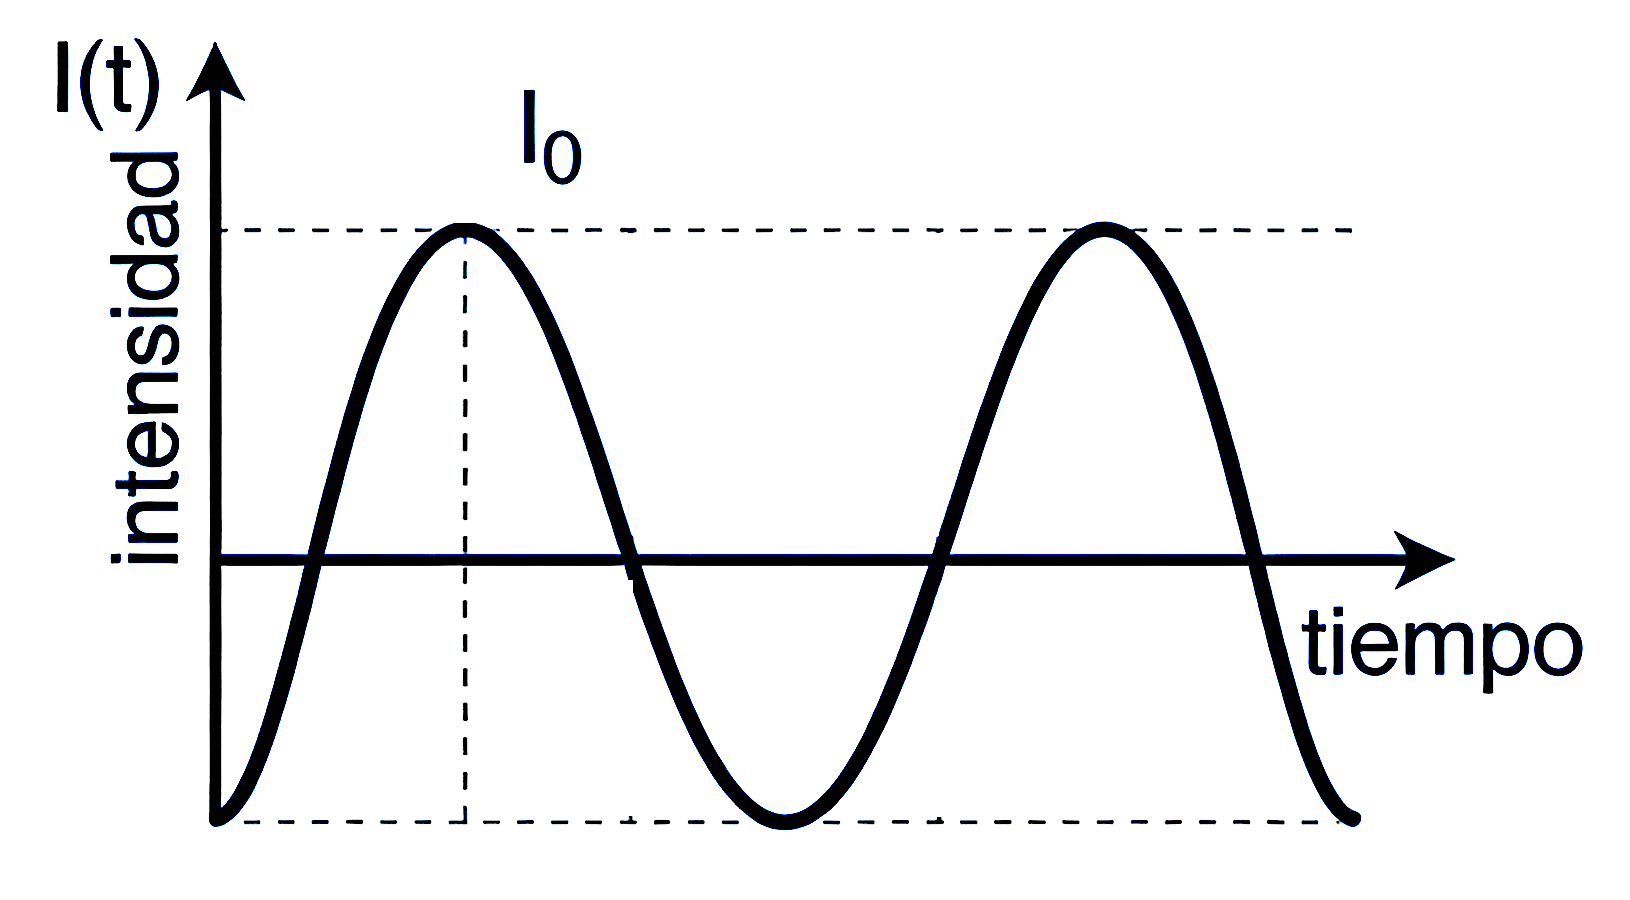
\includegraphics[width=4.16667in,height=\textheight,keepaspectratio]{media/ca.png}

}

\caption{Gráfica de corriente alterna}

\end{figure}%

La corriente alterna es producida por \textbf{inducción} en una espira o
solenoide de \(N\) espiras que gira en el interior de un campo magnético
con velocidad angular \(\omega\). La máquina que genera esta corriente
se denomina \textbf{alternador}. Los símbolos que se suelen utilizar
para representar un alternador en un circuito son los siguientes:

\begin{figure}[H]

{\centering 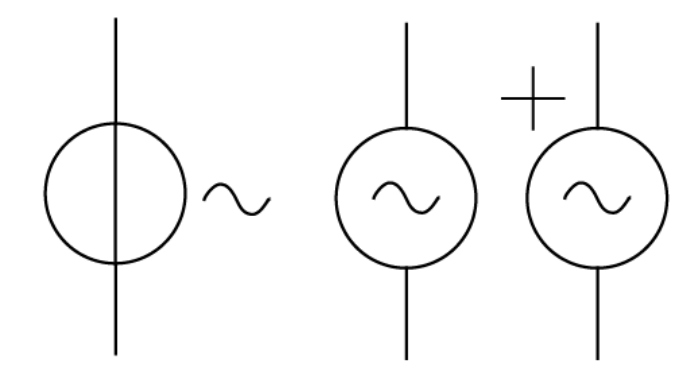
\includegraphics[width=3.625in,height=\textheight,keepaspectratio]{media/simb-fuenteCA.png}

}

\caption{Símbolos de generador de CA}

\end{figure}%

\section{Conceptos fundamentales}\label{conceptos-fundamentales}

\begin{itemize}
\tightlist
\item
  \textbf{Frecuencia:} Es el número de veces que cambia de dirección la
  corriente en un segundo y se mide en \textbf{hercios (Hz)}.
\item
  \textbf{Frecuencia en España:} En nuestro sistema eléctrico se
  utilizan los \textbf{50 Hz}, aunque existen aplicaciones especiales
  (electrónica, radiocomunicaciones) donde se usan frecuencias de kHz o
  MHz.
\item
  \textbf{Transmisión de energía:} Aunque los electrones apenas se
  desplazan unas centésimas de milímetro antes de cambiar de sentido
  (debido a su baja velocidad de deriva), la energía se transmite como
  una \textbf{onda electromagnética} a velocidades cercanas a la de la
  luz, de forma similar a como se propagan las ondas sonoras en el aire.
\end{itemize}

\bookmarksetup{startatroot}

\chapter{Representación de señales
sinusoidales.}\label{representaciuxf3n-de-seuxf1ales-sinusoidales.}

Una señal sinusoidal genérica es aquella que sigue una variación dada
por alguna de las siguientes expresiones:

\[f(t) = A_p \cdot \sin(\omega \cdot t + \varphi)\]
\[f(t) = A_p \cdot \cos(\omega \cdot t + \delta)\]

En la siguiente imagen puedes ver la representación de una función
\textbf{seno} con una amplitud \(A_p\) de 1 y un desfase \(\varphi\) de
30° (\(\pi/6\) radianes) respecto al origen:

\begin{figure}[H]

{\centering 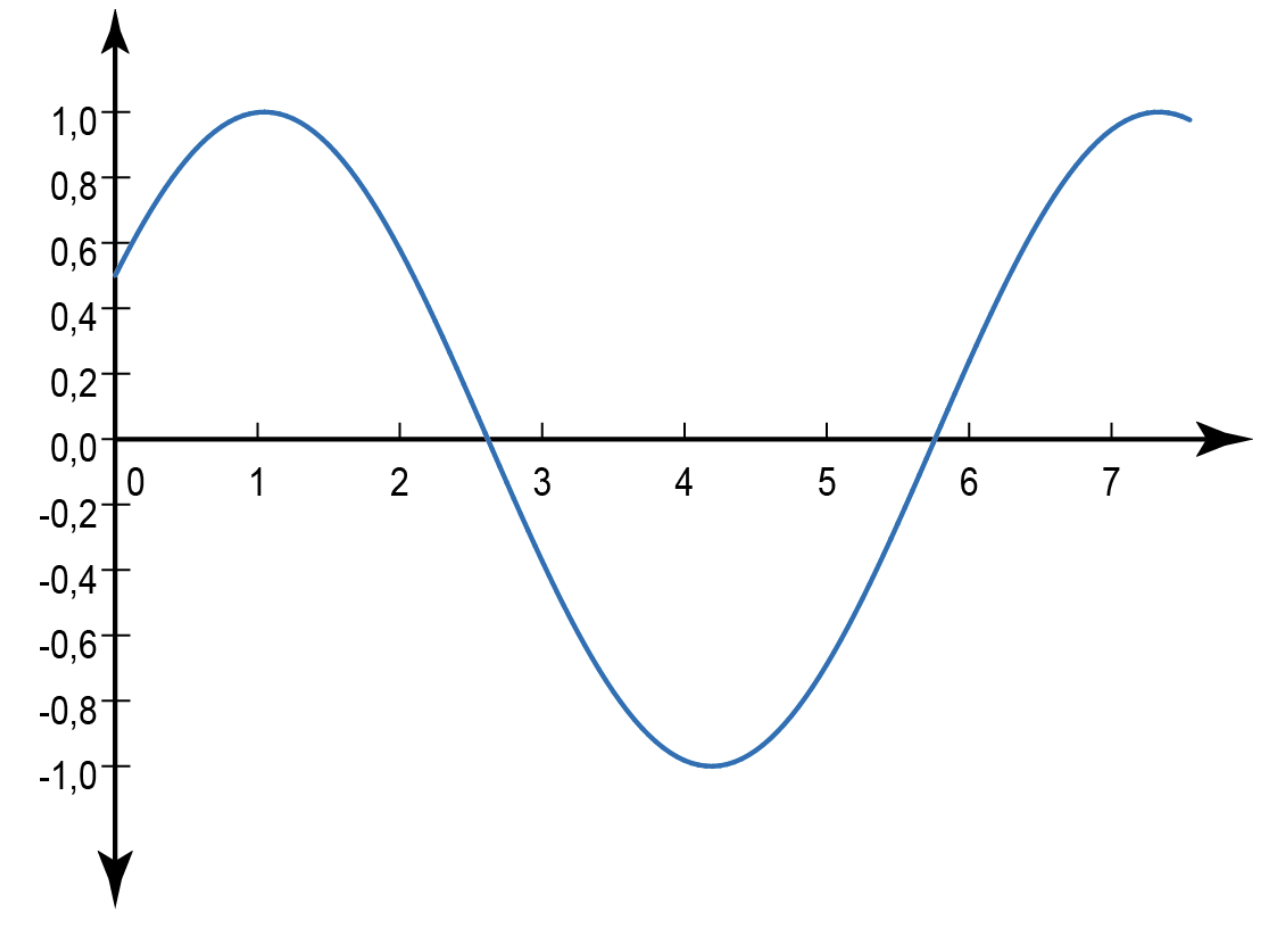
\includegraphics[width=0.7\linewidth,height=\textheight,keepaspectratio]{media/graf-seno.png}

}

\caption{Representación de una función seno con desfase}

\end{figure}%

\begin{tcolorbox}[enhanced jigsaw, breakable, colback=white, left=2mm, leftrule=.75mm, rightrule=.15mm, toprule=.15mm, colframe=quarto-callout-tip-color-frame, arc=.35mm, bottomrule=.15mm, opacityback=0]

\vspace{-3mm}\textbf{Importante}\vspace{3mm}

La representación del coseno sería la misma onda desfasada \(\pi/2\)
radianes (90º) respecto a la anterior. Para simplificar, en este tema
siempre utilizaremos la ley de variación basada en la función
\textbf{seno}.

\end{tcolorbox}

\section{Descripción de una señal
sinusoidal}\label{descripciuxf3n-de-una-seuxf1al-sinusoidal}

Una función sinusoidal es una función periódica porque se repite a
intervalos regulares de tiempo. El tiempo que tarda en repetirse se
llama \textbf{periodo (T)} y se mide en \textbf{segundos (s)}. Se
denomina \textbf{frecuencia} al número de veces que se repite la señal
en un segundo, su unidad es el \textbf{hercio (Hz)}. La relación entre
frecuencia y periodo es inversa: \(f = 1/T\).

Para una señal sinusoidal de la forma
\(f(t) = A_p \cdot \sin(\omega \cdot t + \varphi)\):

\begin{itemize}
\tightlist
\item
  \textbf{\(A_p\)} es la \textbf{amplitud}, es decir, el máximo valor
  que alcanza la señal.
\item
  \textbf{\(\omega\)} es la \textbf{frecuencia angular} o
  \textbf{pulsación} expresada en \textbf{rad/s}, tiene unidades de
  velocidad angular. Su valor es:
  \(\omega = 2\pi \cdot f = \frac{2\pi}{T}\).
\item
  \textbf{\(t\)} es el \textbf{tiempo} medido en \textbf{segundos (s)}.
\item
  \textbf{\(\varphi\)} es el \textbf{ángulo de fase inicial} medido en
  \textbf{radianes (rad)}.
\end{itemize}

Se llama \textbf{ciclo} al conjunto de valores que toma la función en
\textbf{un periodo}. La representación en el tiempo es la utilizada
cuando se estudian señales con un osciloscopio.

\begin{tcolorbox}[enhanced jigsaw, breakable, colback=white, left=2mm, leftrule=.75mm, rightrule=.15mm, toprule=.15mm, colframe=quarto-callout-important-color-frame, arc=.35mm, bottomrule=.15mm, opacityback=0]

\vspace{-3mm}\textbf{Ejemplo de análisis de onda}\vspace{3mm}

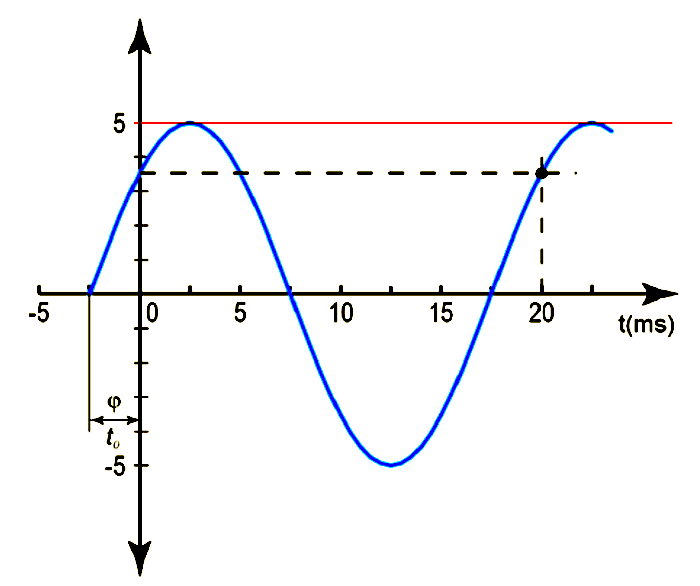
\includegraphics[width=0.5\linewidth,height=\textheight,keepaspectratio]{media/ejemploSinusoidal.png}

\begin{itemize}
\tightlist
\item
  \textbf{Amplitud:} \(A_p = 5\)
\item
  \textbf{Periodo:} \(T = 20 \text{ ms}\)
\item
  \textbf{Frecuencia:} \(f = 1/T = 50 \text{ Hz}\)
\item
  \textbf{Pulsación:} \(\omega = 2\pi \cdot f = 100\pi \text{ rad/s}\)
\item
  \textbf{Fase inicial, \(\varphi\):} La fase inicial está señalada en
  la figura; es necesario expresarla en radianes, no en tiempo. Para
  relacionar ambos sabemos que el periodo \(T\) se corresponde con un
  ángulo de \(2\pi\) radianes; según esto se puede establecer que:
  \[\varphi = \frac{2\pi \cdot t_{0}}{T} = \frac{2\pi \cdot 2,5}{20} = \frac{\pi}{4} \text{ rad}\]
\end{itemize}

La expresión que define la señal del ejemplo será, por lo tanto:

\[f(t)=5\cdot\sen\left(100\pi t+\frac{\pi}{4}\right)\]

\end{tcolorbox}

\section{Valores significativos de una señal
sinusoidal}\label{valores-significativos-de-una-seuxf1al-sinusoidal}

\textbf{Valor instantáneo}

Es el valor que tiene la onda en cada instante. Se puede calcular
evaluando la expresión matemática en un instante de tiempo \(t\)
determinado.

\textbf{Valor de pico o valor de cresta}

Es el valor máximo que toma la señal, es decir, su amplitud.

\textbf{Valor medio}

Es la media aritmética de todos los valores instantáneos que pueden
darse en un periodo. Se calcula matemáticamente así:

\[U_m = \frac{1}{T} \int_0^T u(t)\,dt\]

En el caso de la señal seno, el valor medio sería cero~al ser una
función simétrica. Por lo tanto, se utiliza el valor medio en un
semiperiodo (T/2), que sí tiene un valor útil y que tiene esta
expresión:

\[U_m = \frac{1}{T/2} \int_0^{T/2} u(t)\,dt\]

\textbf{Valor eficaz}

Aunque el valor medio de la intensidad sea cero, eso no significa que no
haya movimiento de electrones ni consumo de energía en una resistencia
R. Los electrones están constantemente realizando un movimiento de
vibración cambiando de sentido en cada semiperiodo. Este movimiento hace
que, por efecto Joule, consuman energía en la resistencia,
independientemente del sentido del movimiento.

La potencia consumida será

\[P(t) = R\,I^2 = R\,I_0^2\sen^2(\omega t)\]

Y la energía consumida en un periodo, por tanto, será

\[E = \int_{0}^{T}P(t)dt= \int_{0}^{T} R\,I_0^2\sen^2(\omega t) dt=R\,I_0^2\frac{T}{2}\]

Si comparamos este resultado con una corriente continua que consumiera
la misma energía (es decir, si estudiamos el problema ``como si la
corriente fuera continua'', circulando una intensidad Ie):

\[E = R\,I_e^2T\]

Vemos que la intensidad de corriente continua necesaria para consumir la
misma energía que la corriente alterna es:

\[I_{e}^{2}=\frac{I_{0}^{2}}{2}\Rightarrow I_{e}=\frac{I_{0}}{\sqrt{2}}\]

Este valor se denomina \textbf{valor eficaz}, y es el más usado al
estudiar circuitos de corriente alterna ya que, como ya veremos, usando
valores eficaces sí se cumple la ley de Ohm, cosa que no ocurre con los
valores instantáneos, debido al desfase.

Del mismo modo que la intensidad eficaz es
\(I_{e}=\frac{I_{0}}{\sqrt{2}}\), el voltaje eficaz es
\(V_{e}=\frac{V_{0}}{\sqrt{2}}\)

\section{Representación fasorial y
compleja}\label{representaciuxf3n-fasorial-y-compleja}

Una magnitud sinusoidal se puede representar como la proyección vertical
de un \textbf{vector rotativo (fasor)} que gira a una velocidad angular
\(\omega\) en sentido contrario al de las agujas del reloj. Su módulo es
igual al valor de cresta (\(U_p\)) y su posición inicial es la fase
inicial (\(\varphi\)).

\begin{figure}[H]

{\centering 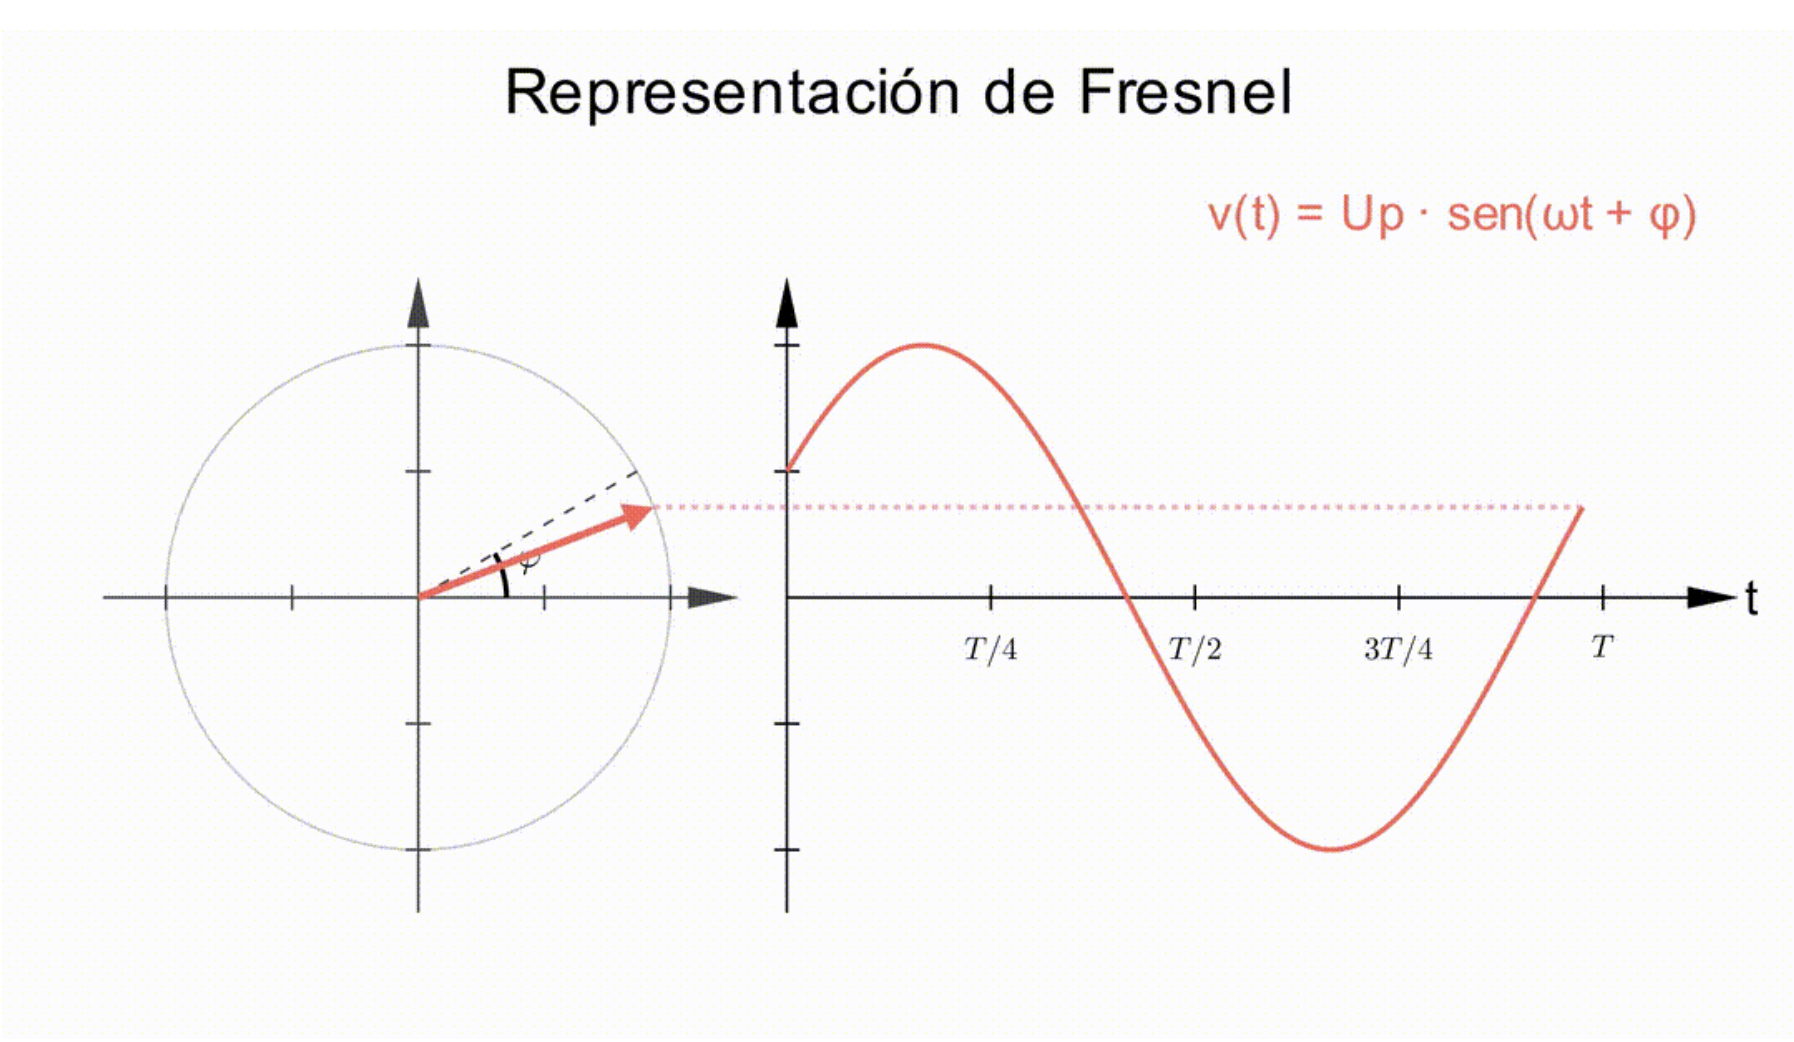
\includegraphics[width=0.8\linewidth,height=\textheight,keepaspectratio]{media/FresnelGenerico.png}

}

\caption{Imagen del concepto de fasor}

\end{figure}%

\subsection{Formas de expresar un
fasor}\label{formas-de-expresar-un-fasor}

\textbf{Nota sobre notación:} Al tratarse de una magnitud vectorial, a
partir de ahora utilizaremos la notación de vector con flecha (ej.
\(\vec{U}, \vec{I}\)) para referirnos al fasor completo (número
complejo), distinguiéndolo así claramente de su módulo o valor escalar
(ej. \(U, I\)).

\begin{itemize}
\tightlist
\item
  \textbf{Forma polar:} \(\vec{U} = U_{p} \angle \varphi\).
\item
  \textbf{Forma compleja:}
  \(\vec{U} = U_{p} \cos \varphi + j \cdot U_{p} \sin \varphi\). Donde
  \(j=\sqrt{-1}\) es la \emph{unidad imaginaria}, que en Electrotecnia
  se denomina \textbf{\(j\)} para no confundirla con la intensidad.
  Representa un \textbf{giro de +90°} en el diagrama fasorial.
\end{itemize}

\begin{tcolorbox}[enhanced jigsaw, breakable, colback=white, left=2mm, leftrule=.75mm, rightrule=.15mm, toprule=.15mm, colframe=quarto-callout-important-color-frame, arc=.35mm, bottomrule=.15mm, opacityback=0]

\vspace{-3mm}\textbf{Ejemplo: Representación de una corriente}\vspace{3mm}

Representa gráficamente la siguiente señal correspondiente a una
corriente:

\[i(t)=3\cdot \sen(10\pi t-\frac{\pi}{3})\]

Solución:

Debemos representar un vector de módulo 3, con un desfase inicial
\(\varphi=-\frac{\pi}{3} \, \text{rad}\) o \(\varphi=-60º\). Este vector
giraría a una velocidad \(\omega=10\pi \, \text{rad/s}\).

La representación polar es la siguiente:

\[\vec{I}=I_{p}\angle \varphi=3\phase{-60º} \, \text{A}\]

o, expresando el ángulo en radianes:

\[\vec{I}=I_{p}\angle \varphi=3\phase{-\pi /3} \, \text{A}\]

La representación en forma de número complejo es:

\[\vec{I}=I_{p}\cos \varphi + j \cdot I_{p} \sen \varphi=3·\cos(-60º)+j·3·\sen(-60º)=1,5-1,5\sqrt{3}j\, \text{A}\]

Y, por último, la representación gráfica sería:

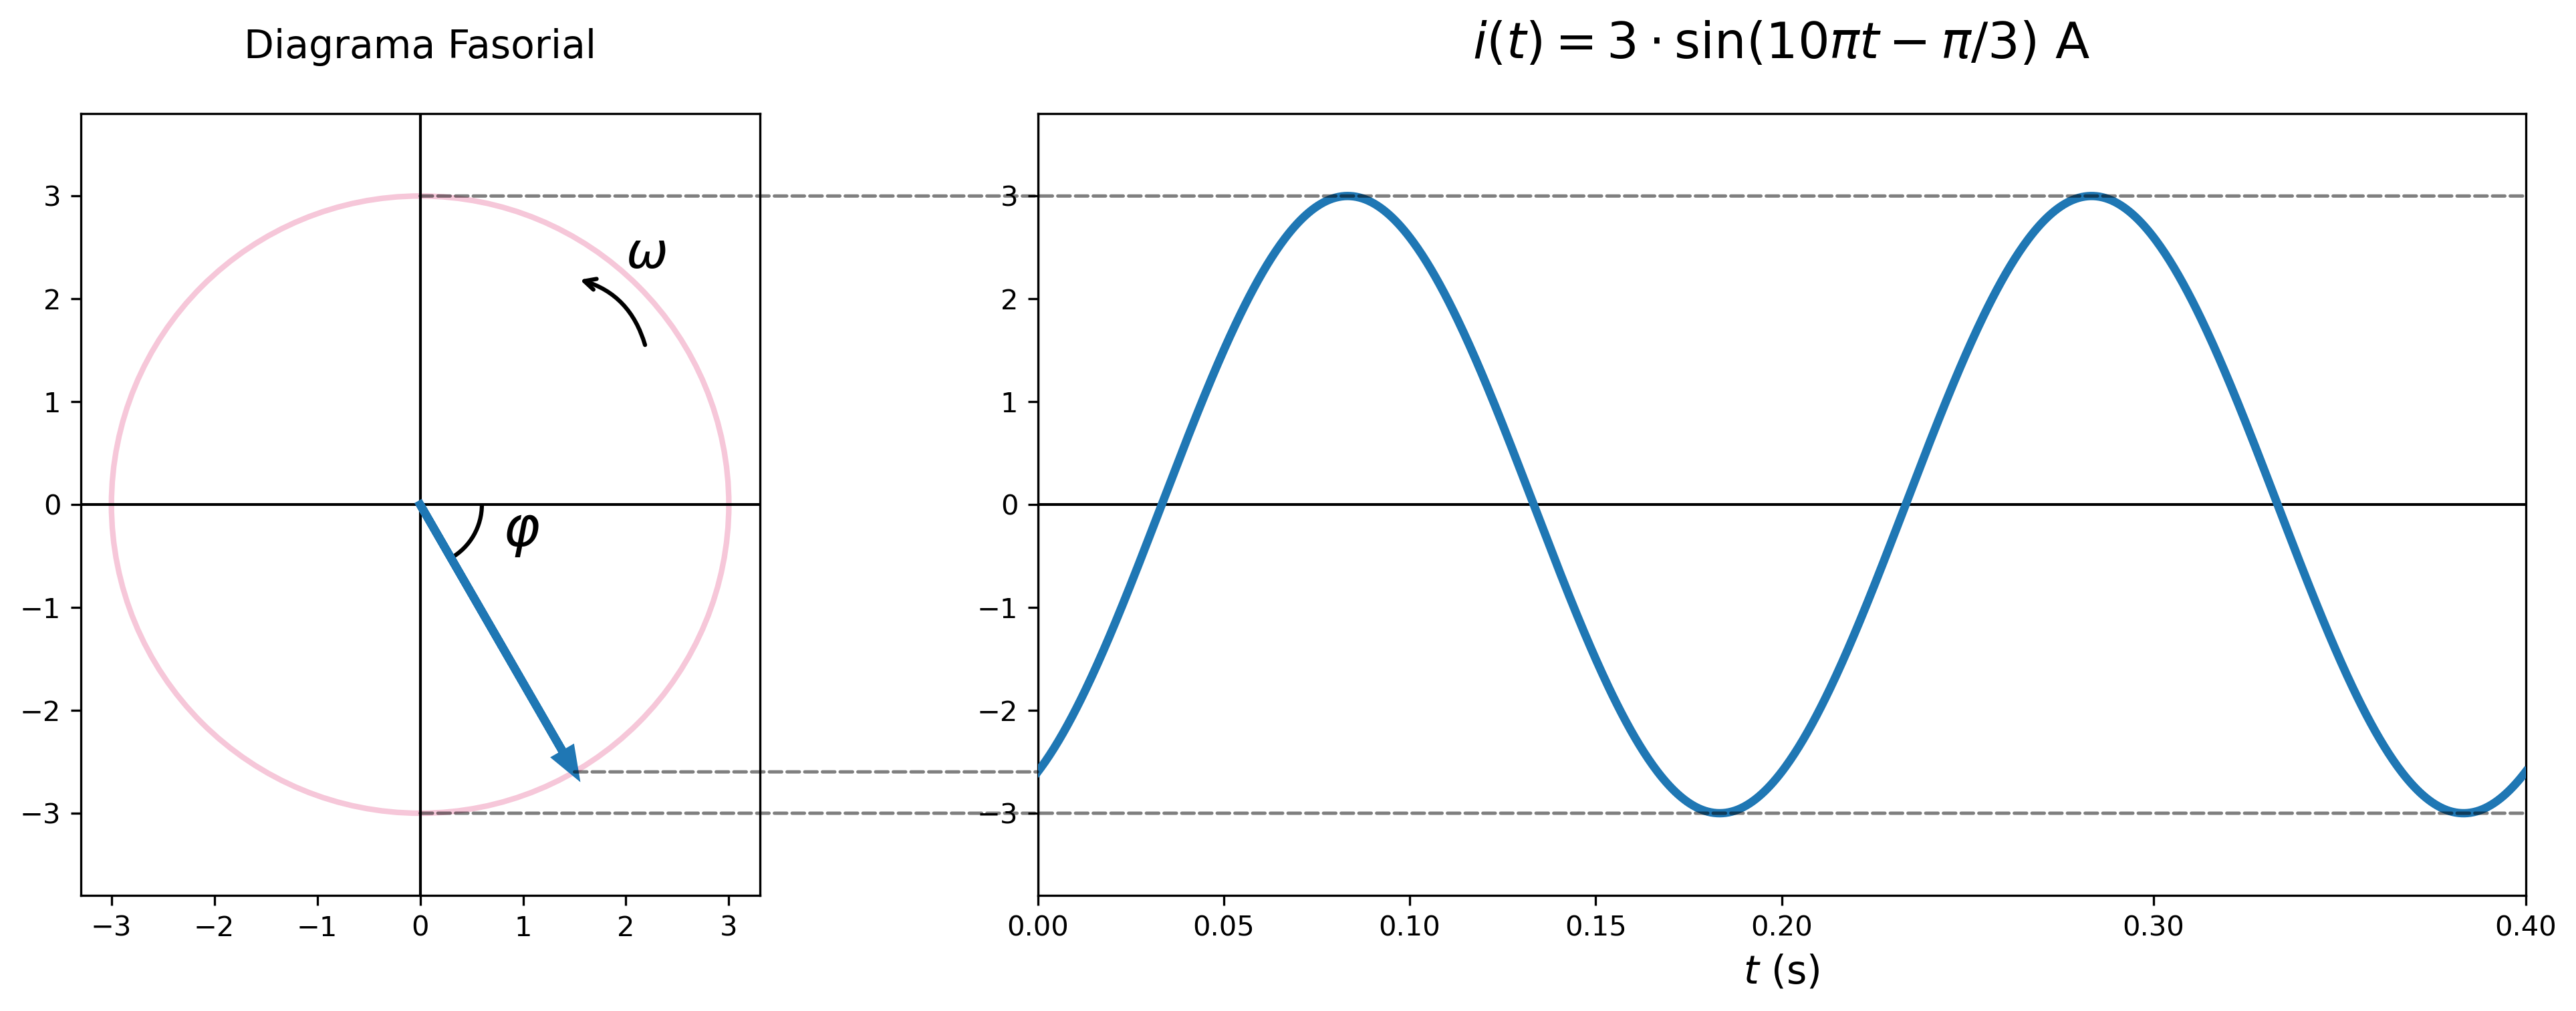
\includegraphics[width=0.7\linewidth,height=\textheight,keepaspectratio]{media/fasor_final_blanco.png}

\end{tcolorbox}

\bookmarksetup{startatroot}

\chapter{Respuesta de los componentes básicos a la Corriente
Alterna}\label{respuesta-de-los-componentes-buxe1sicos-a-la-corriente-alterna}

\section{Respuesta de una
resistencia}\label{respuesta-de-una-resistencia}

Si a una resistencia de valor R ohmios (Ω) se la somete a una tensión
sinusoidal de \textbf{valor eficaz U} y \textbf{pulsación ω}, la tensión
instantánea aplicada a la resistencia es:
\[u(t) = (\sqrt{2} U) \cdot \sen(\omega t + \varphi)\]

Según la ley de Ohm, tenemos que \(i(t) = u(t)/R\), y por tanto, la
intensidad instantánea que circula por la resistencia es:
\[i(t) = \frac{\sqrt{2}U}{R} \cdot \sen(\omega  t + \varphi)\]
Analizando las expresiones de la tensión y la intensidad, podemos
concluir que:

\begin{itemize}
\tightlist
\item
  La intensidad eficaz es \(I=\frac{U}{R}\), igual que en corriente
  continua.
\item
  El desfase entre la tensión y la intensidad es nulo. Es decir, están
  en fase (\(\varphi_{I}=\varphi\))
\end{itemize}

La representación gráfica de la tensión y la intensidad en una
resistencia eléctrica será, por tanto:

\begin{center}
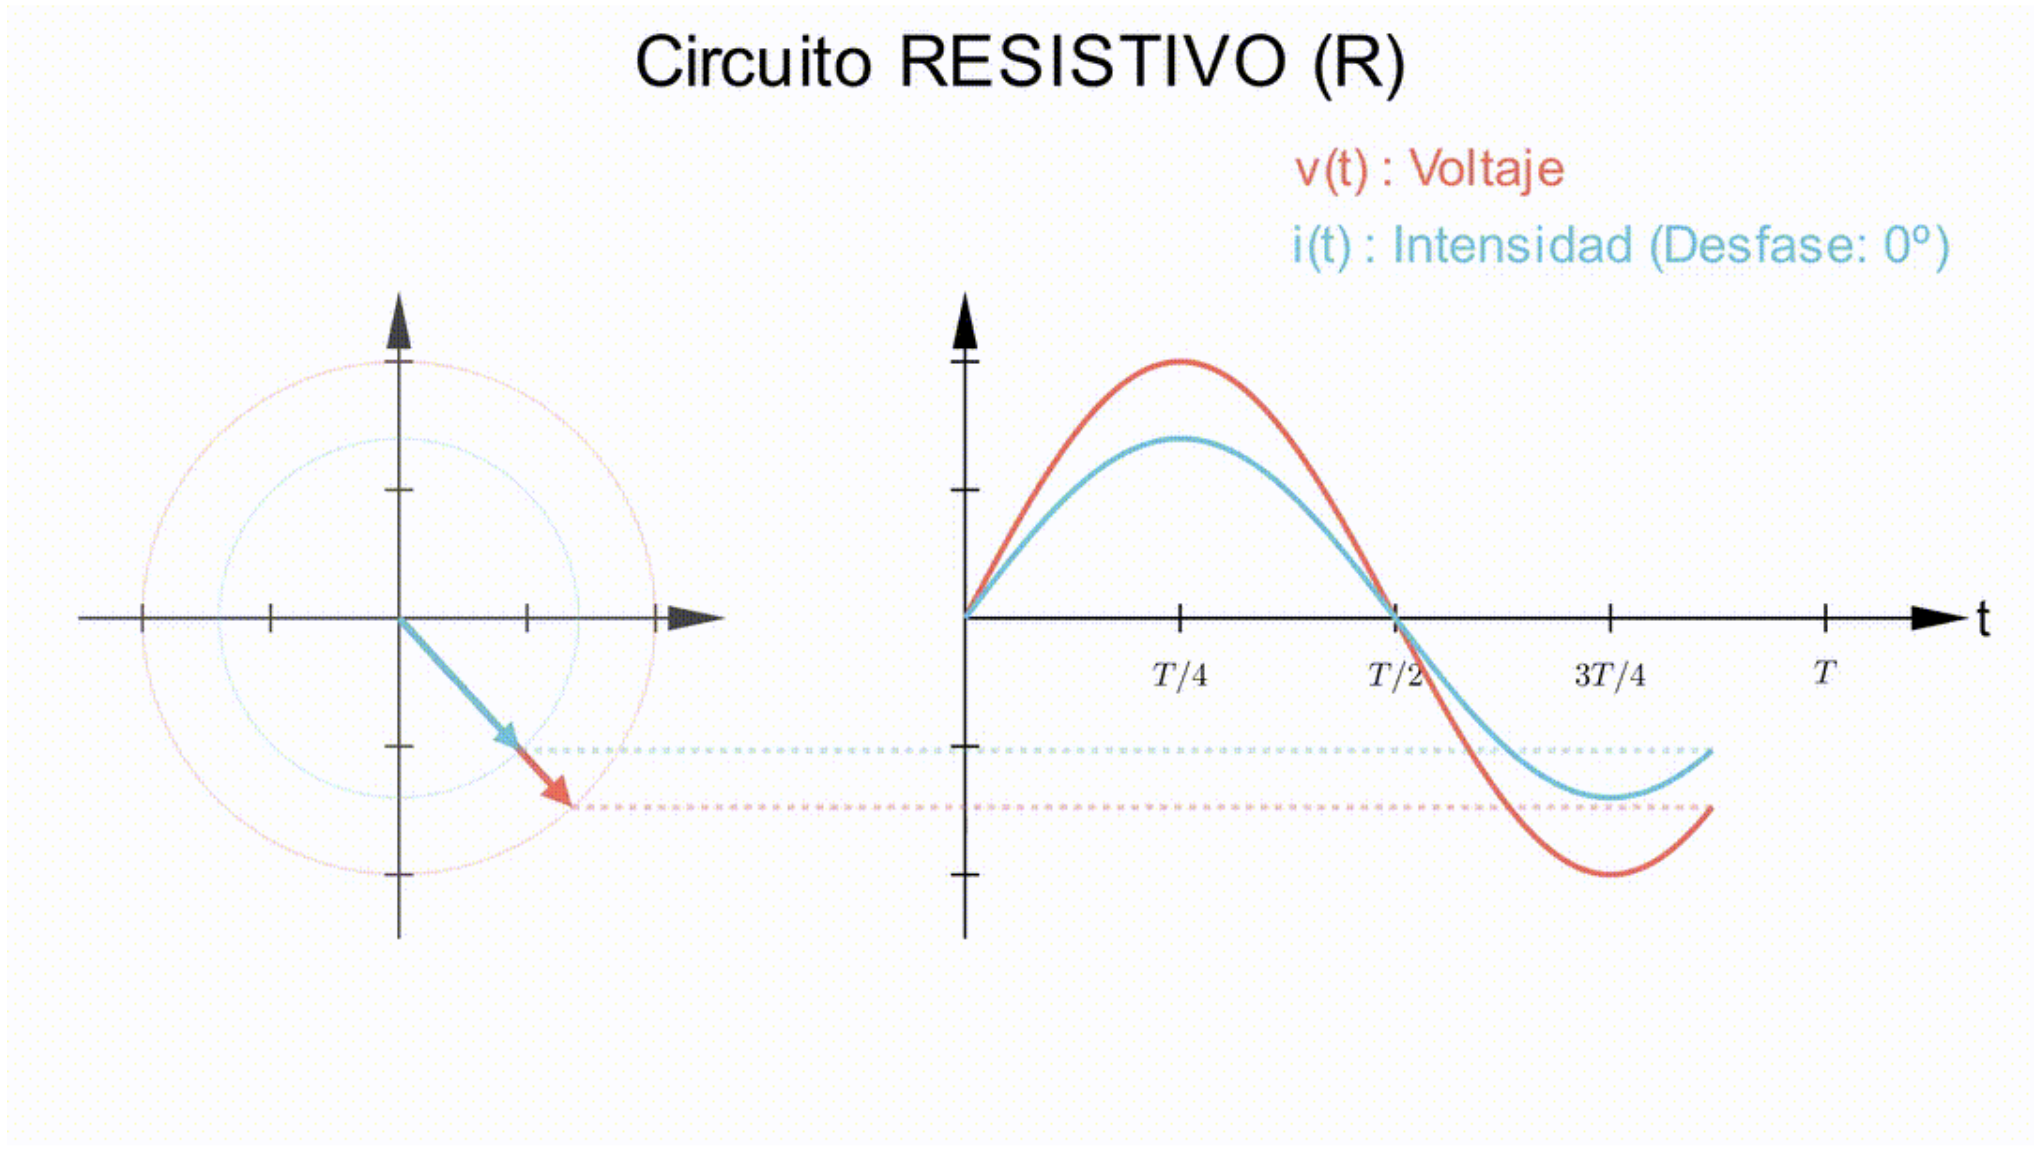
\includegraphics[width=0.9\linewidth,height=\textheight,keepaspectratio]{media/FresnelResistivo.png}
\end{center}

\section{Respuesta de una bobina}\label{respuesta-de-una-bobina}

La característica básica de una bobina es su \textbf{inductancia}, que
se denota mediante la letra \textbf{L} y se mide en \textbf{Henrios
(H)}. En corriente alterna, sin embargo, no basta con este valor sino
que su respuesta será diferente para distintas frecuencias de
funcionamiento.

Si a una bobina de valor \textbf{L henrios (H)} se la somete a una
intensidad sinusoidal de \textbf{valor eficaz U} y \textbf{pulsación ω},
la intensidad instantánea que circula por la bobina es:

\[
i(t) = (\sqrt{2}I) \cdot \sen(\omega t + \varphi)
\]

La ley que rige para una bobina es la siguiente:

\[u(t) = L \cdot \frac{di(t)}{dt}\]

Por lo tanto, la tensión instantánea en la bobina la obtenemos derivando
la intensidad y resulta ser:

\[u(t) = L \frac{di(t)}{dt} = L \cdot (\sqrt{2}I) \cdot \omega \cdot \sen(\omega  t + \varphi + \frac{\pi}{2})\]

\begin{tcolorbox}[enhanced jigsaw, breakable, colback=white, left=2mm, leftrule=.75mm, rightrule=.15mm, toprule=.15mm, colframe=quarto-callout-note-color-frame, arc=.35mm, bottomrule=.15mm, opacityback=0]

\vspace{-3mm}\textbf{Importante}\vspace{3mm}

En realidad, la derivada del seno es el coseno, pero el coseno de un
ángulo es igual al seno de su complementario
(\(\cos(\alpha) = \sen(\alpha + \frac{\pi}{2})\)). Por lo tanto, podemos
poner la expresión en forma de seno, para poder comparar los fasores de
la tensión y la intensidad.

\end{tcolorbox}

Por consiguiente, obtenemos una tensión con la misma pulsación que la
intensidad y con las características siguientes:

\begin{itemize}
\item
  Un valor de pico \(U_p=\omega \cdot L \cdot \sqrt{2} I\). Por lo
  tanto, \textbf{la tensión eficaz es}
  \(U=\omega \cdot L \cdot I\)\textbf{.}
\item
  La tensión se encuentra adelantada 90° (\$\textbackslash pi/2 \$ ) con
  respecto a la intensidad; la \textbf{fase inicial de la tensión es}
  \(\varphi_U = \varphi + \frac{\pi}{2}\)\textbf{.}
\end{itemize}

Al producto \(\omega \cdot L\) se le llama \textbf{reactancia inductiva}
y se representa por \(X_L\), es decir:

\begin{tcolorbox}[enhanced jigsaw, breakable, colback=white, left=2mm, leftrule=.75mm, rightrule=.15mm, toprule=.15mm, colframe=quarto-callout-caution-color-frame, arc=.35mm, bottomrule=.15mm, opacityback=0]

\[
X_L=\omega \cdot L
\]

\end{tcolorbox}

\textbf{La unidad de la reactancia inductiva en el SI es el ohmio
(}\(\omega\)\textbf{).}

La representación gráfica de los fasores y ondas de tensión e intensidad
en una bobina es la mostrada en la figura:

\begin{center}
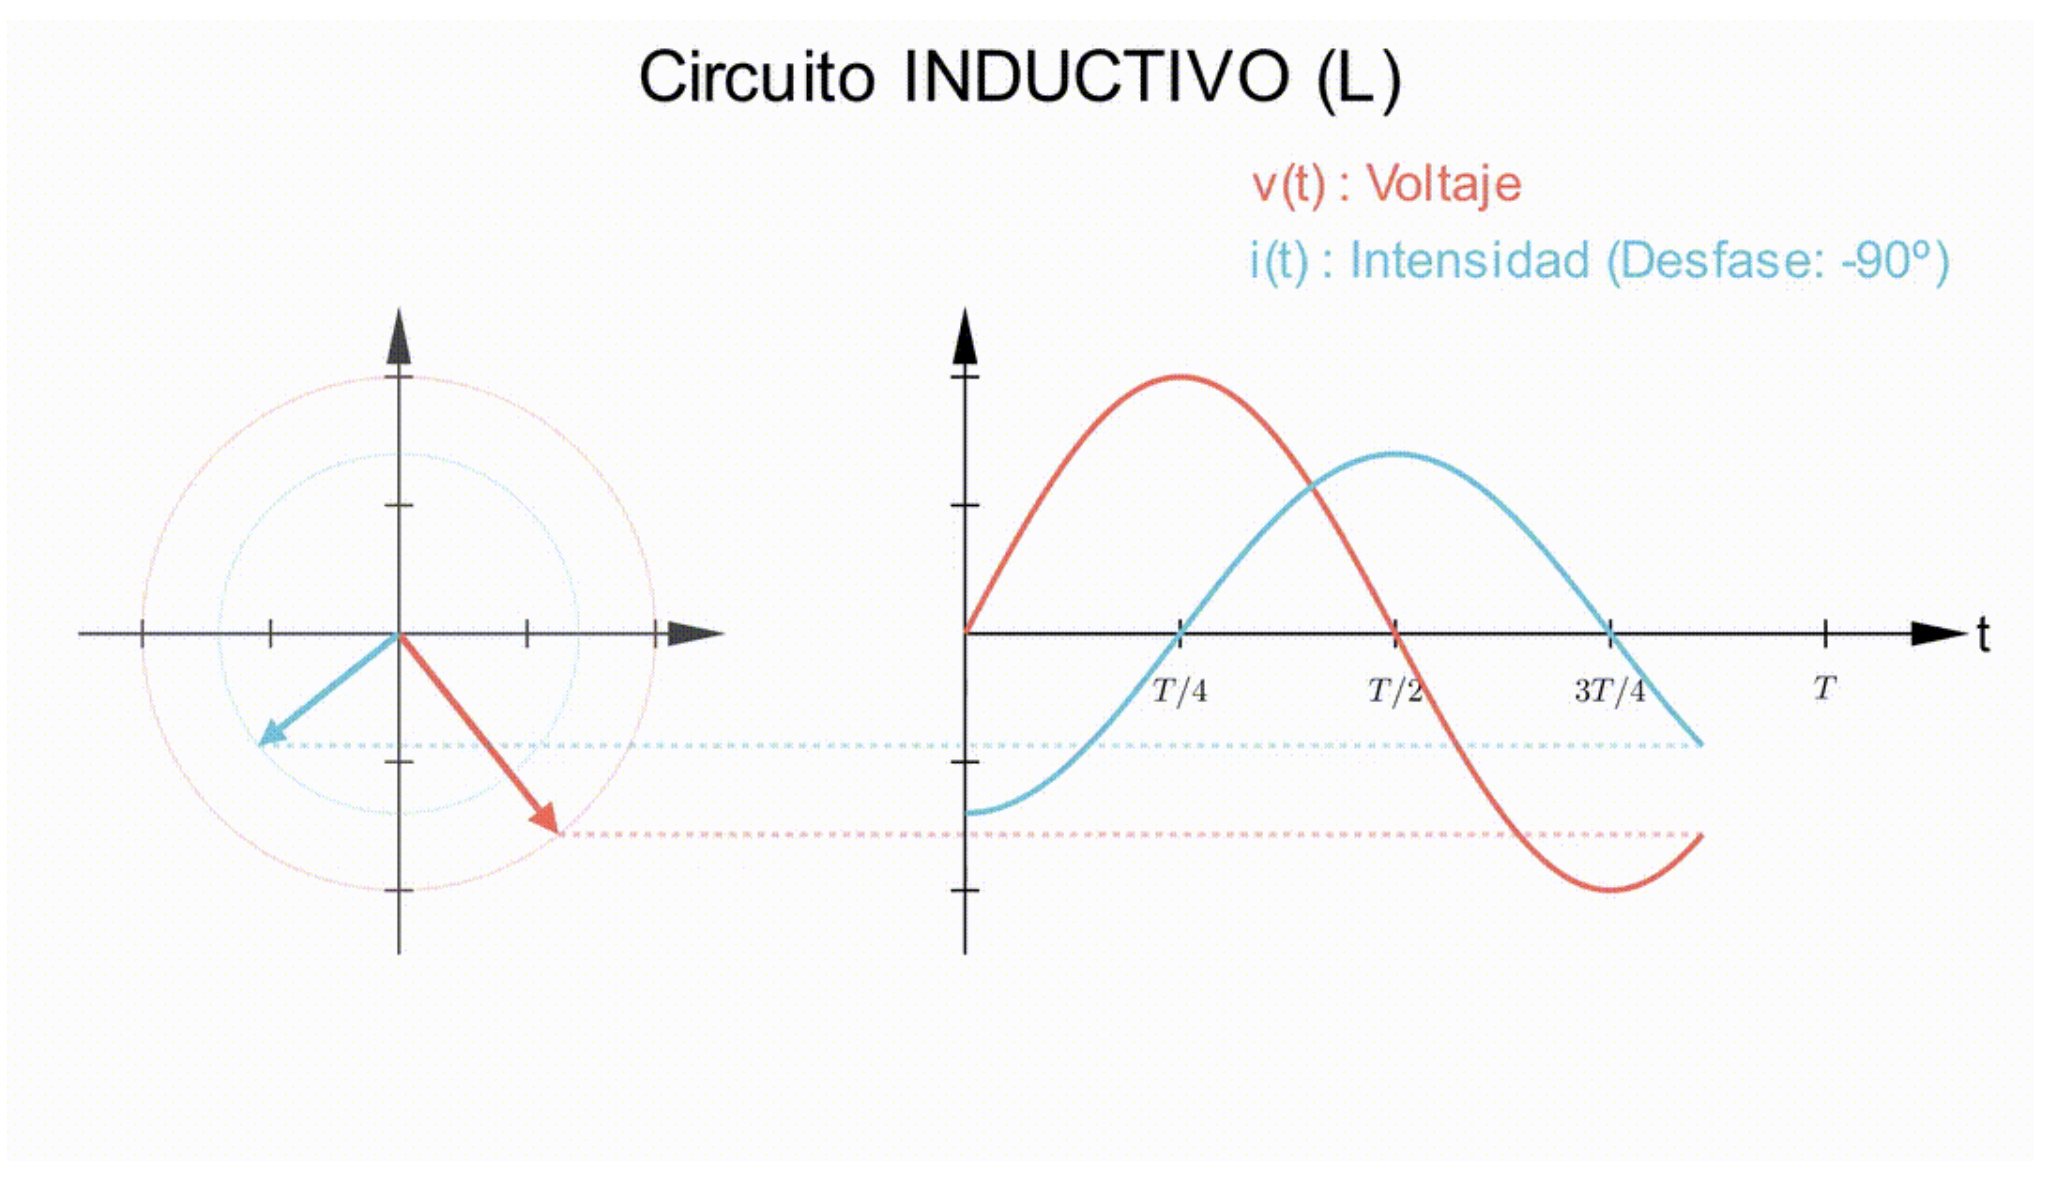
\includegraphics[width=0.9\linewidth,height=\textheight,keepaspectratio]{media/FresnelInductivo.png}
\end{center}

\section{Respuesta de un condensador}\label{respuesta-de-un-condensador}

La característica básica de un condensador es su \textbf{capacitancia} o
capacidad, que se denota mediante la letra \textbf{C} y se mide en
\textbf{Faradios (F)}. En corriente alterna, sin embargo, no basta con
este valor sino que su respuesta será diferente para distintas
frecuencias de funcionamiento.

Si a un condensador de valor \textbf{C faradios (F)} se le somete a una
tensión sinusoidal de valor eficaz U y pulsación co, la tensión
instantánea aplicada al condensador es:
\[u(t) = (\sqrt{2} U) \cdot \sen(\omega t + \varphi)\]

Aplicando la ley que rige un condensador, \(i(t) = C \cdot du(t) / dt\),
la intensidad instantánea que circula por el condensador es: \[
i(t) = C \cdot \frac{du(t)}{dt} = C \cdot \omega \cdot ( \sqrt{2}U) \cdot \sen(\omega  t + \varphi + \frac{\pi}{2})
\]

Obtenemos una intensidad con la misma pulsación que la tensión aplicada
y con las características siguientes:

\begin{itemize}
\tightlist
\item
  Un valor de pico \(I_p=\omega \cdot C \cdot \sqrt{2} U\). Por lo
  tanto, \textbf{la intensidad eficaz es}
  \(I=\omega \cdot C \cdot U\)\textbf{.}
\item
  La intensidad se encuentra adelantada 90° (\(\pi/2\)) con respecto a
  la tensión; la \textbf{fase inicial de la intensidad es}
  \(\varphi_I = \varphi + \frac{\pi}{2}\)\textbf{.}
\end{itemize}

Al cociente \(1/\omega \cdot C\) se le llama \textbf{reactancia
capacitiva} y se representa por \(X_C\), es decir:

\begin{tcolorbox}[enhanced jigsaw, breakable, colback=white, left=2mm, leftrule=.75mm, rightrule=.15mm, toprule=.15mm, colframe=quarto-callout-caution-color-frame, arc=.35mm, bottomrule=.15mm, opacityback=0]

\[
X_C=\frac{1}{\omega \cdot C}
\]

\end{tcolorbox}

\textbf{La unidad de la reactancia capacitiva en el SI es el ohmio
(}\(\omega\)\textbf{).}

La representación gráfica de los fasores y ondas de tensión e intensidad
en un condensador es la mostrada en la figura:

\begin{center}
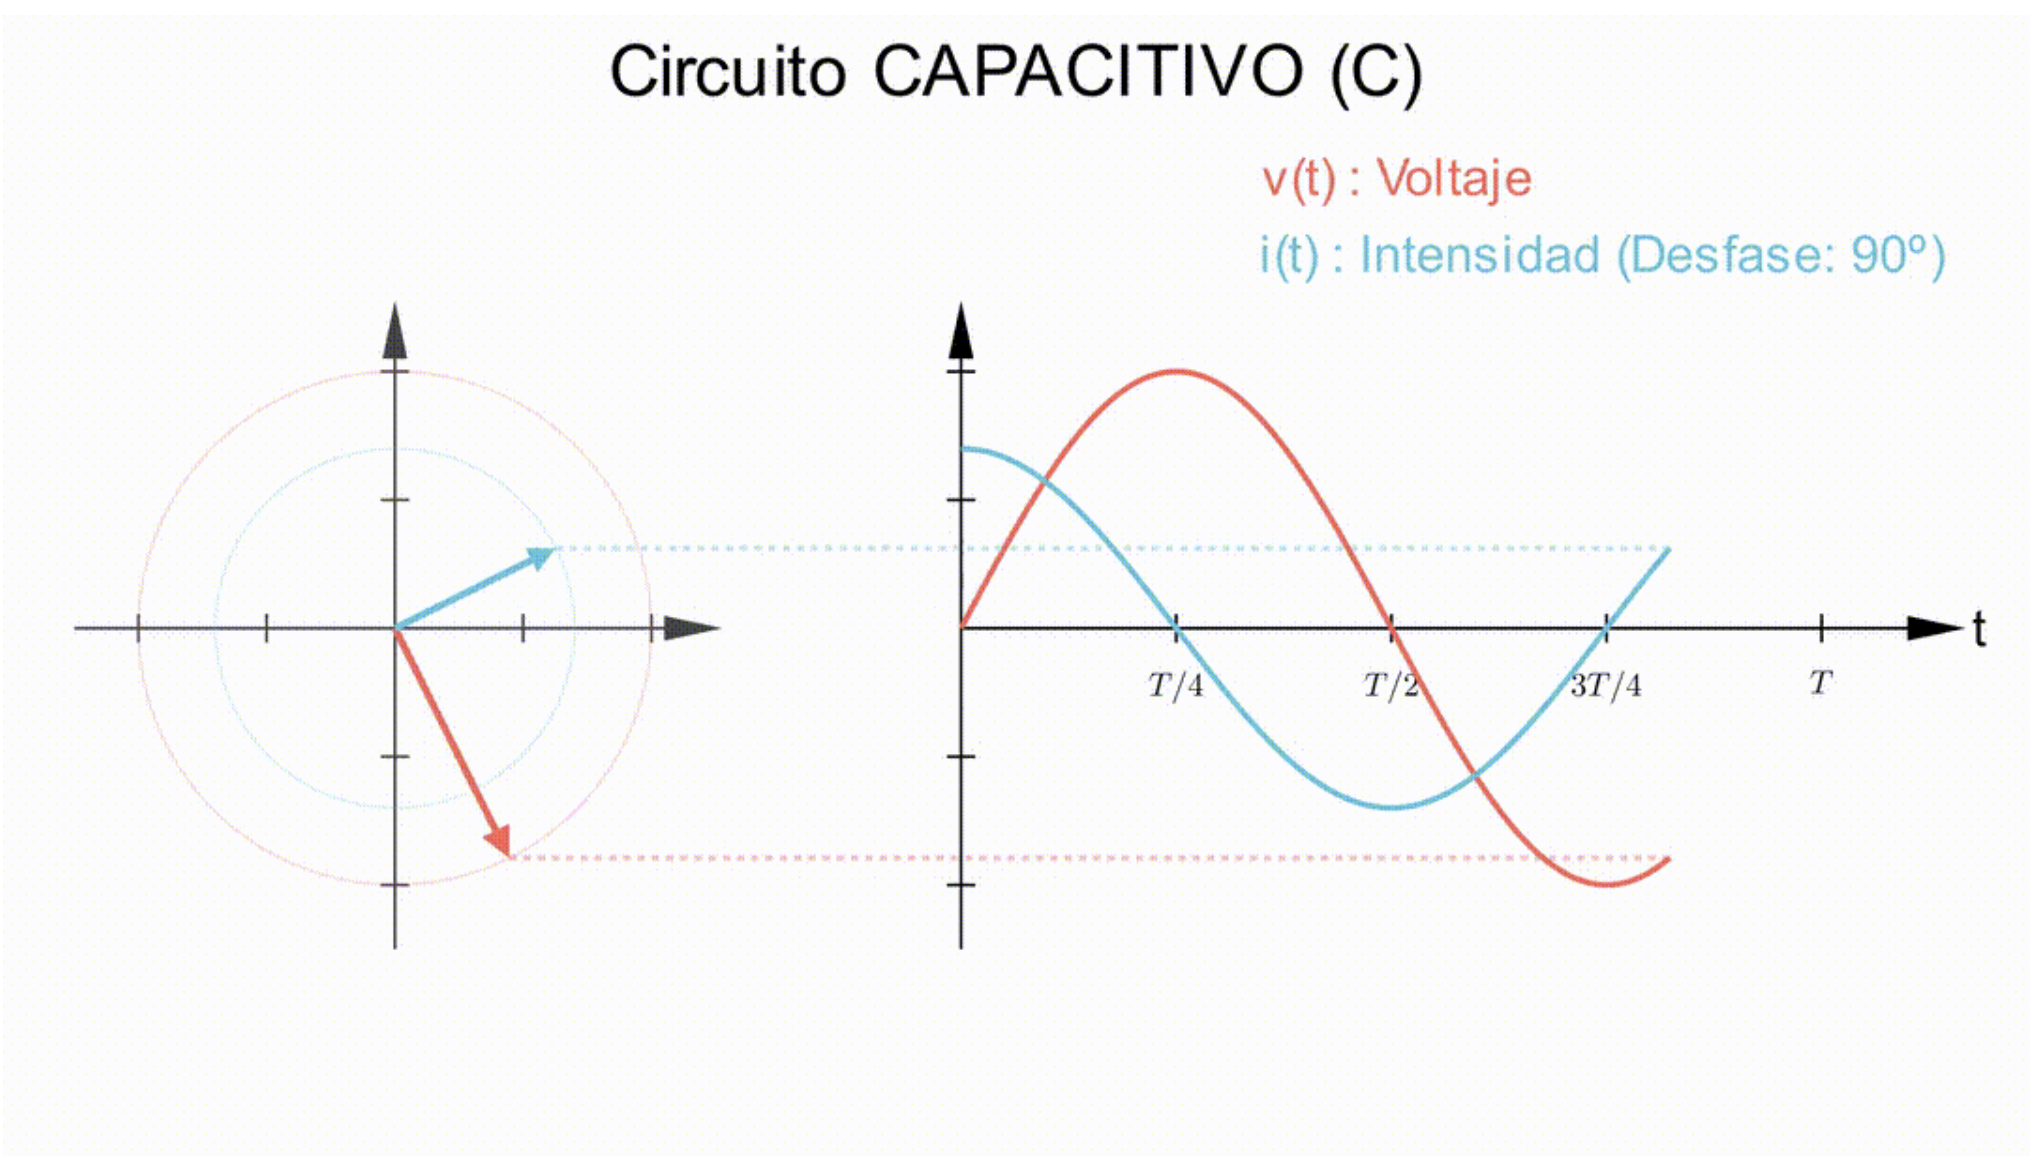
\includegraphics[width=0.9\linewidth,height=\textheight,keepaspectratio]{media/FresnelCapacitivo.png}
\end{center}

\section{Cuadro resumen con las respuestas R, L y
C}\label{cuadro-resumen-con-las-respuestas-r-l-y-c}

\begin{longtable}[]{@{}
  >{\centering\arraybackslash}p{(\linewidth - 6\tabcolsep) * \real{0.2500}}
  >{\centering\arraybackslash}p{(\linewidth - 6\tabcolsep) * \real{0.2500}}
  >{\centering\arraybackslash}p{(\linewidth - 6\tabcolsep) * \real{0.2500}}
  >{\centering\arraybackslash}p{(\linewidth - 6\tabcolsep) * \real{0.2500}}@{}}
\toprule\noalign{}
\begin{minipage}[b]{\linewidth}\centering
Elemento
\end{minipage} & \begin{minipage}[b]{\linewidth}\centering
Representación gráfica
\end{minipage} & \begin{minipage}[b]{\linewidth}\centering
Relación Tensión/Intensidad
\end{minipage} & \begin{minipage}[b]{\linewidth}\centering
Desfase rad (º)
\end{minipage} \\
\midrule\noalign{}
\endhead
\bottomrule\noalign{}
\endlastfoot
\textbf{Resistencia (\(R\))} &
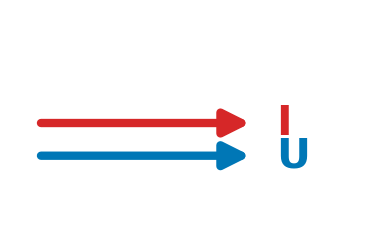
\includegraphics[width=1.04167in,height=\textheight,keepaspectratio]{media/icono_fasor_R.png}
& \(R\) & \(0^\circ\) \\
\textbf{Bobina (\(L\))} &
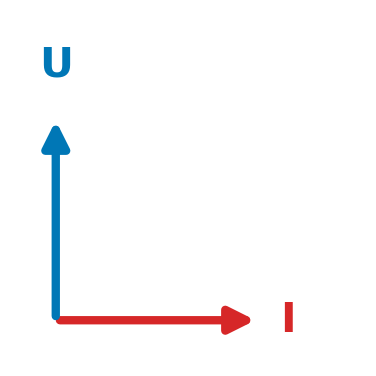
\includegraphics[width=1.04167in,height=\textheight,keepaspectratio]{media/icono_fasor_L.png}
& \(X_L = \omega \cdot L\) & \(+\pi/2 \ (+90^\circ)\) \\
\textbf{Condensador (\(C\))} &
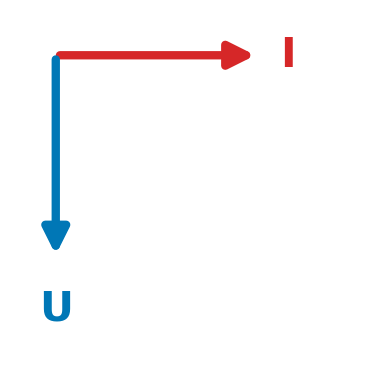
\includegraphics[width=1.04167in,height=\textheight,keepaspectratio]{media/icono_fasor_C.png}
& \(X_C = \frac{1}{\omega \cdot C}\) & \(-\pi/2 \ (-90^\circ)\) \\
\end{longtable}

\section{Combinación de cargas de diferente
naturaleza}\label{combinaciuxf3n-de-cargas-de-diferente-naturaleza}

Por lo general, en un circuito tendremos cargas que ofrecerán diferentes
resistencias eléctricas. Además, algunas presentarán también carácter
inductivo o capacitivo. Dependiendo de la combinación de elementos que
tengamos en cada circuito, el desfase entre la intensidad y la tensión
podrá tomar diferentes valores, no solo 0º, -90º o +90º. En este
simulador puedes ver cómo cambiarían los fasores de la tensión y la
intensidad dependiendo de cómo variemos las componentes R, L o C de un
circuito:

\section{Simulación Interactiva}\label{simulaciuxf3n-interactiva}

Como este documento es estático, no es posible mostrar la simulación
interactiva de los fasores giratorios. Puedes acceder a la versión
animada haciendo clic en el siguiente enlace:

\begin{figure}[H]

{\centering 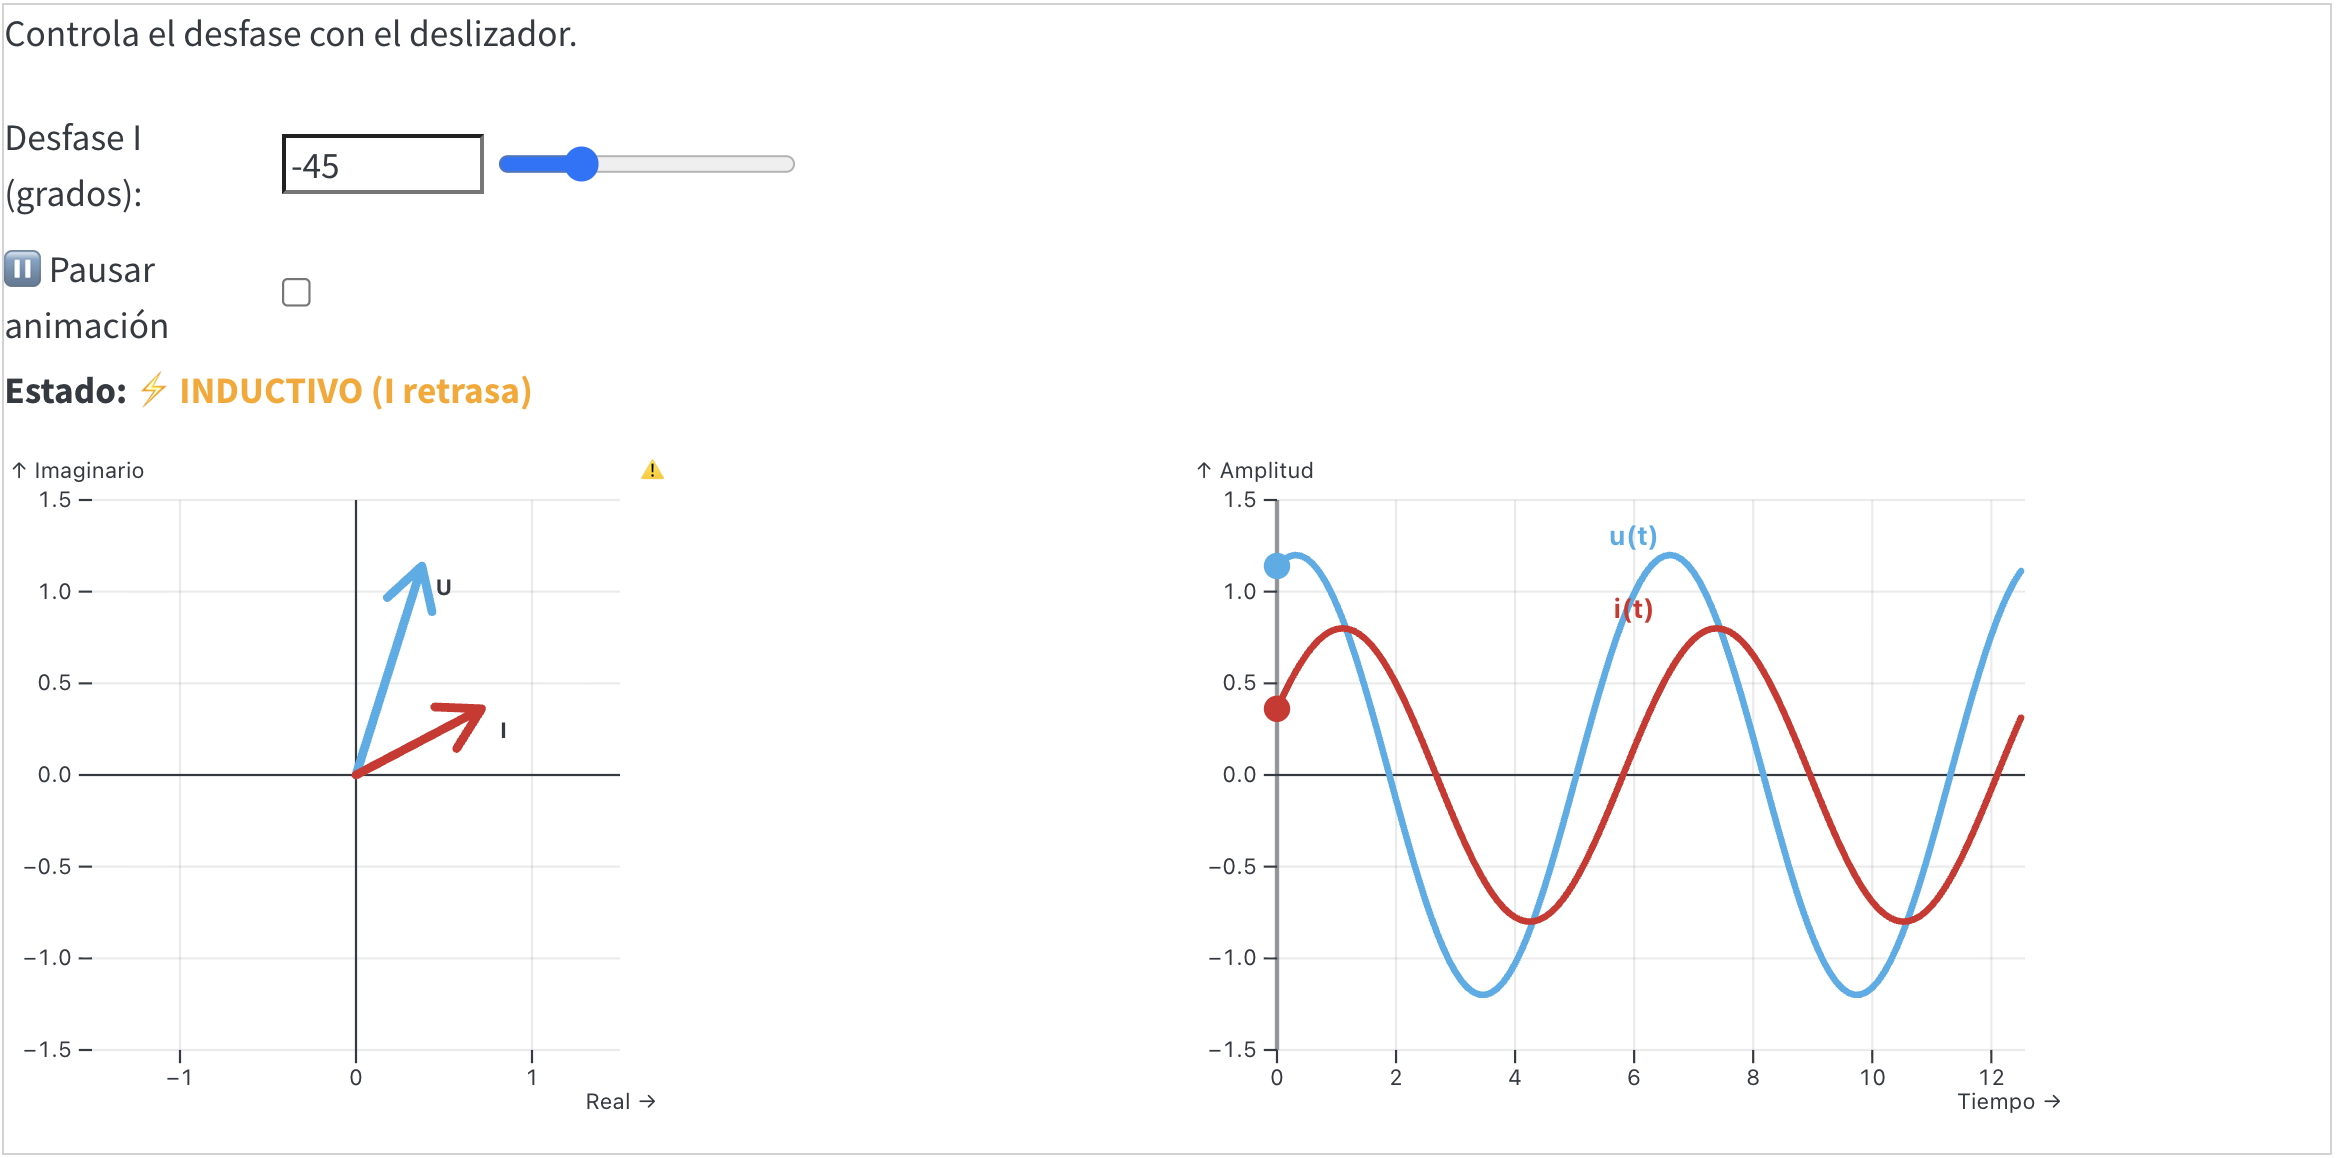
\includegraphics[width=0.8\linewidth,height=\textheight,keepaspectratio]{media/sim_fasores.png}

}

\caption{Captura de la simulación}

\end{figure}%

\href{https://joselugarEducaAnd.github.io/2teci-circuitosCA/03_respuesta_comp.html}{\textbf{➡️
Ver Simulación Interactiva en la Web}}

\bookmarksetup{startatroot}

\chapter{Impedancia}\label{impedancia}

El concepto de impedancia es una \textbf{generalización del concepto de
resistencia.} Hemos visto que en CA los elementos conectados en el
circuito, en general, introducen un desfase entre la intensidad y la
tensión. Este desfase hace que no haya una proporcionalidad entre los
valores instantáneos de intensidad y tensión, como ocurría en corriente
continua.

No se cumple la ley de Ohm, tal y como la conocíamos, con los valores
instantáneos \(i(t)\) y \(v(t)\). Sin embargo, \textbf{esta
proporcionalidad sí existe entre los fasores}, y también entre los
valores máximos \(U_0\) e \(I_0\), o los valores eficaces \(U\), \(I\).
Esto hace que podamos expresar la ley de Ohm con estos valores.

La magnitud que relaciona los valores máximos (y los eficaces) de
tensión e intensidad en un circuito, se denomina impedancia (\(Z\)), y
se mide en ohmios.

La resistencia eléctrica de un conductor se define como la oposición que
ofrece al paso de una corriente eléctrica. Cuando la corriente que
atraviesa a un conductor es una corriente sinusoidal, el concepto de
resistencia se generaliza a impedancia.

\begin{tcolorbox}[enhanced jigsaw, breakable, colback=white, left=2mm, leftrule=.75mm, rightrule=.15mm, toprule=.15mm, colframe=quarto-callout-warning-color-frame, arc=.35mm, bottomrule=.15mm, opacityback=0]

\vspace{-3mm}\textbf{Definición}\vspace{3mm}

La \textbf{impedancia} de un conductor se define como la
\textbf{oposición} que ofrece al paso de una corriente eléctrica
\textbf{sinusoidal}.

\end{tcolorbox}

La impedancia se representa con la letra \(\vec{Z}\). Consideremos una
impedancia \(\vec{Z}\) alimentada por una señal sinusoidal de valor
eficaz \(U\), fase inicial \(\varphi_U\) y pulsación \(\omega\), tal
como se muestra en la figura:

\begin{figure}[H]

{\centering 
\includegraphics[width=4.16667in,height=\textheight,keepaspectratio]{media/circuito1.png}

}

\caption{Circuito con Impedancia}

\end{figure}%

La tensión en la impedancia, que es la de la fuente, representada en
forma de fasor es: \[\vec{U} = \sqrt{2}U \phase \varphi_U\]

La intensidad que circula por la impedancia tiene un valor eficaz \(I\)
y un desfase \(\varphi_I\). Representada en forma de fasor la intensidad
es: \[\vec{I} = \sqrt{2}I \phase \varphi_I\]

El cociente entre el fasor tensión y el fasor intensidad representa la
impedancia. Expresado matemáticamente es:

\[
\vec{Z}=\frac{\vec{U}}{\vec{I}}=\frac{\sqrt{2}U \phase \varphi_U}{\sqrt{2}I \phase \varphi_I}=\frac{U}{I}\phase {\varphi_U-\varphi_I}
\]

\subsection{La Ley de Ohm
Generalizada}\label{la-ley-de-ohm-generalizada}

De forma análoga a la corriente continua, en corriente alterna existe
una relación lineal fundamental entre la tensión y la intensidad, pero
operando con \textbf{números complejos} (fasores).

\begin{tcolorbox}[enhanced jigsaw, breakable, colback=white, left=2mm, leftrule=.75mm, rightrule=.15mm, toprule=.15mm, colframe=quarto-callout-warning-color-frame, arc=.35mm, bottomrule=.15mm, opacityback=0]

\vspace{-3mm}\textbf{⚡ Ley de Ohm para Corriente Alterna}\vspace{3mm}

La intensidad que recorre un circuito o componente de corriente alterna
es igual al cociente entre la tensión fasorial aplicada y su impedancia
compleja.

\[
\vec{I} = \frac{\vec{U}}{\vec{Z}}
\]

Donde:

\begin{itemize}
\tightlist
\item
  \(\vec{I}\): Es el fasor Intensidad (A).
\item
  \(\vec{U}\): Es el fasor Tensión (V).
\item
  \(\vec{Z}\): Es la Impedancia Compleja (\(\Omega\)).
\end{itemize}

\end{tcolorbox}

Esta expresión vectorial implica dos igualdades escalares separadas:

\begin{enumerate}
\def\labelenumi{\arabic{enumi}.}
\tightlist
\item
  \textbf{En Módulos:} La relación entre los valores eficaces.
  \[I = \frac{U}{|\vec{Z}|} = \frac{U}{Z}\]
\item
  \textbf{En Argumentos (Ángulos):} El desfase de la intensidad es el de
  la tensión menos el de la impedancia.
  \[\varphi_I = \varphi_U - \varphi_Z\]
\end{enumerate}

\section{Triángulo de impedancias}\label{triuxe1ngulo-de-impedancias}

\begin{tcolorbox}[enhanced jigsaw, breakable, colback=white, left=2mm, leftrule=.75mm, rightrule=.15mm, toprule=.15mm, colframe=quarto-callout-note-color-frame, arc=.35mm, bottomrule=.15mm, opacityback=0]

\vspace{-3mm}\textbf{Observación}\vspace{3mm}

Una impedancia \textbf{no es un fasor} (no gira con el tiempo), pero se
representa matemáticamente mediante un \textbf{número complejo} (vector
fijo). Este vector, expresado en forma polar, contiene dos términos:

\begin{itemize}
\tightlist
\item
  El \textbf{módulo (}\(Z\)), que representa el cociente entre la
  tensión y la intensidad que soporta la impedancia. Las tensiones o
  intensidades pueden darse en valores eficaces o en valores de pico.
\item
  El \textbf{argumento (}\(\varphi\)), que representa el \textbf{desfase
  entre el fasor tensión y el fasor intensidad}.
\end{itemize}

\end{tcolorbox}

Si dibujamos ese vector, podremos ver gráficamente que la componente
horizontal correspondería con la \textbf{resistencia} y la vertical con
la \textbf{reactancia} (si es positiva sería inductiva y si es negativa
sería capacitiva) del circuito. Esta representación se denomina
``triángulo de impedancias'' y tiene este aspecto:

\begin{figure}[H]

{\centering 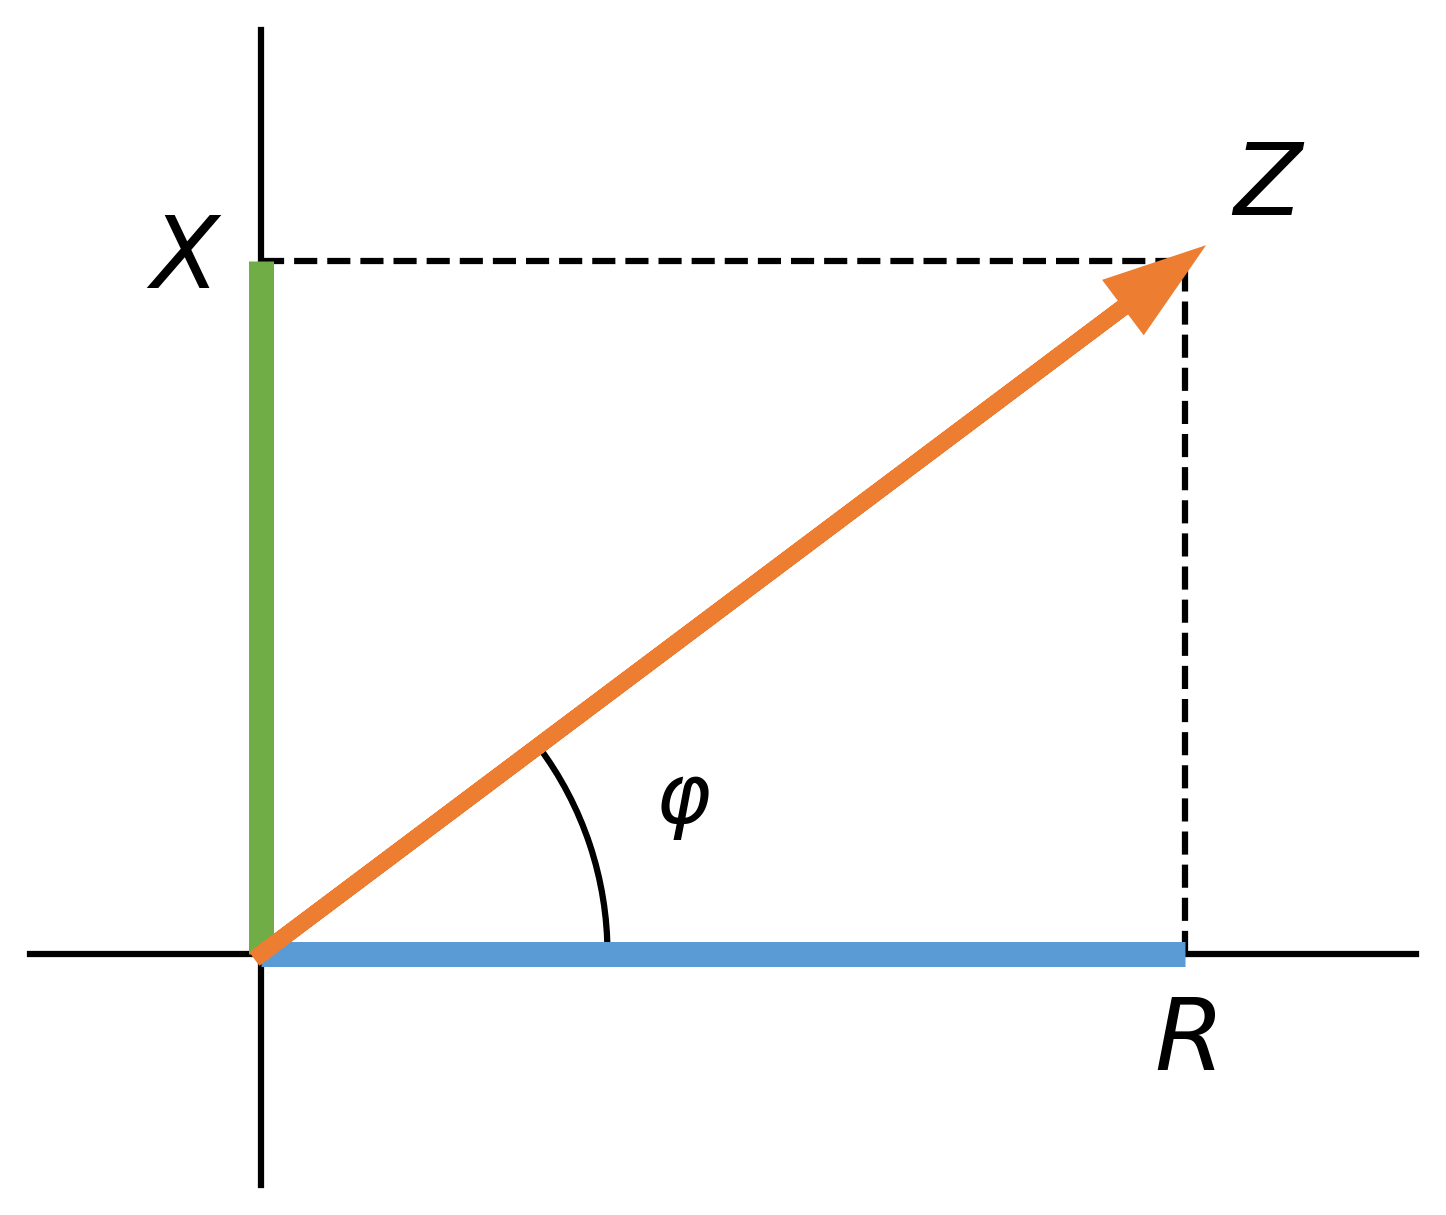
\includegraphics[width=4.16667in,height=\textheight,keepaspectratio]{media/triangulo_impedancias.png}

}

\caption{Triángulo de impedancias}

\end{figure}%

Viendo esta imagen podemos concluir que:

\begin{itemize}
\item
  A partir de la impedancia, podemos calcular la resistencia y la
  reactancia: \[
  R=Z \cdot \cos \varphi
  \] \[
  X=Z \cdot \sen \varphi
  \]
\item
  A partir de la resistencia y la reactancia, podemos calcular la
  impedancia: \[
  |\vec{Z}|=Z=\sqrt{R^2+X^2}
  \] \[
  \varphi = \arctan \frac{X}{R}
  \]
\end{itemize}

\section{Representación compleja de la
impedancia}\label{representaciuxf3n-compleja-de-la-impedancia}

Teniendo en cuenta que el eje horizontal es el eje real y el eje
vertical es el eje imaginario, podemos representar el vector impedancia
como un número complejo de la forma: \[ 
\vec{Z} = R + \mathrm{j} \cdot X 
\]

Recordemos que:

\begin{itemize}
\tightlist
\item
  \(R\) \textbf{es la resistencia:} se mide en ohmios
  (\(\mathrm{\omega}\)) y se puede calcular como
  \(R=Z \cdot \cos \varphi\).
\item
  \(X\) \textbf{es la reactancia:} se mide también en ohmios
  (\(\mathrm{\omega}\)) y se puede calcular como
  \(R=Z \cdot \sen \varphi\). Según el valor que tome la reactancia, la
  impedancia puede ser:

  \begin{itemize}
  \tightlist
  \item
    \textbf{Impedancia inductiva:} cuando \(X>0\) y, por lo tanto
    \(\varphi >0\), \textbf{la tensión está en avance con respecto a la
    intensidad.}
  \item
    \textbf{Impedancia capacitiva:} cuando \(X<0\) y, por lo tanto,
    \(\varphi <0\), \textbf{la tensión está en retraso con respecto a la
    intensidad} o, lo que lo mismo, la intensidad va por delante de la
    tensión.
  \end{itemize}
\end{itemize}

\begin{tcolorbox}[enhanced jigsaw, breakable, colback=white, left=2mm, leftrule=.75mm, rightrule=.15mm, toprule=.15mm, colframe=quarto-callout-important-color-frame, arc=.35mm, bottomrule=.15mm, opacityback=0]

\vspace{-3mm}\textbf{Ejemplo}\vspace{3mm}

\textbf{Determina el valor de la resistencia y reactancia de una
impedancia que está sometida a una tensión de 220 V y por la que circula
una intensidad de 10 A. Se sabe que la tensión está adelantada 30º con
respecto a la intensidad.}

\emph{Solución:}

Aplicando la definición de impedancia (en módulos), tenemos:
\[Z = \frac{U}{I} = \frac{220}{10} = 22 \ \Omega\]

Tenemos una parte de la impedancia, pero falta saber qué desfase existe.
Este dato nos lo dan con el desfase entre la tensión e intensidad,
\(\varphi = \varphi_U - \varphi_I\), así \(\varphi = 30^\circ\). La
impedancia expresada en forma polar vectorial es:
\[\vec{Z} = 22 \phase 30^\circ \ \Omega\]

Para obtener \(R\) y \(X\) hacemos: \[
\begin{aligned}
R &= Z \cdot \cos \varphi = 22 \cdot \cos(30^\circ) = 11\sqrt{3} \ \Omega \\
X &= Z \cdot \sen \varphi = 22 \cdot \sen(30^\circ) = 11 \ \Omega
\end{aligned}
\quad \Rightarrow \quad
\boxed{
\begin{aligned}
R &= 11 \cdot \sqrt{3} \ \Omega \\
X &= 11 \ \Omega
\end{aligned}
}
\]

Se trata de una reactancia \textbf{inductiva}.

\end{tcolorbox}

\vspace{1em}

\begin{tcolorbox}[enhanced jigsaw, breakable, colback=white, left=2mm, leftrule=.75mm, rightrule=.15mm, toprule=.15mm, colframe=quarto-callout-warning-color-frame, arc=.35mm, bottomrule=.15mm, opacityback=0]

\vspace{-3mm}\textbf{Importante}\vspace{3mm}

La \textbf{representación compleja} de las impedancias resistiva,
inductiva y capacitiva es la siguiente:

\[
\begin{aligned}
\vec{Z}_R &= R \\[1ex]
\vec{Z}_L &= \mathrm{j} \cdot X_L = \mathrm{j} \cdot \omega \cdot L \\[1ex]
\vec{Z}_C &= -\mathrm{j} \cdot X_C = \frac{-\mathrm{j}}{\omega \cdot C}
\end{aligned}
\]

\end{tcolorbox}

\vspace{1em}

\begin{tcolorbox}[enhanced jigsaw, breakable, colback=white, left=2mm, leftrule=.75mm, rightrule=.15mm, toprule=.15mm, colframe=quarto-callout-tip-color-frame, arc=.35mm, bottomrule=.15mm, opacityback=0]

\vspace{-3mm}\textbf{¿Necesitas repasar los Números Complejos?}\vspace{3mm}

Para trabajar con impedancias usaremos \textbf{fasores} y
\textbf{números complejos} continuamente. Si no recuerdas cómo operar
con ellos (suma, producto, paso a polar\ldots), consulta el
\textbf{\hyperref[sec-anexo-complejos]{Anexo de Matemáticas}} al final
del libro.

\end{tcolorbox}

\section{Asociación de impedancias}\label{asociaciuxf3n-de-impedancias}

Las impedancias se pueden asociar de la misma forma en que se asociaban
las resistencias: asociación en serie, en paralelo y mixta.

\begin{itemize}
\item
  \textbf{Asociación en serie:} la impedancia equivalente es la suma
  vectorial de las impedancias parciales. \[
    \vec{Z}_T=\vec{Z}_1+\vec{Z}_2+\vec{Z}_3+...
    \]
\item
  \textbf{Asociación en paralelo:} la inversa de la impedancia
  equivalente es la suma de las inversas de las impedancias parciales,
  es decir: \[
    \frac{1}{\vec{Z}_T}=\frac{1}{\vec{Z}_1}+\frac{1}{\vec{Z}_2}+\frac{1}{\vec{Z}_3}+...
    \]
\item
  \textbf{Asociación mixta:} es una combinación de serie y paralelo.
  Aunque veremos algunos casos, serán muy sencillos y los resolveremos
  como serie puro y luego paralelo o viceversa.
\end{itemize}

\begin{tcolorbox}[enhanced jigsaw, breakable, colback=white, left=2mm, leftrule=.75mm, rightrule=.15mm, toprule=.15mm, colframe=quarto-callout-warning-color-frame, arc=.35mm, bottomrule=.15mm, opacityback=0]

\vspace{-3mm}\textbf{Importante}\vspace{3mm}

A diferencia de las resistencias, las impedancias son \textbf{números
complejos}. Para sumar impedancias (caso de una conexión en serie)
debemos \textbf{sumar las partes reales (resistencias) e imaginarias
(reactancias) por separado}, para luego calcular el valor de la
impedancia (\(\vec{Z}\)) y del desfase total (\(\varphi\)) aplicando lo
visto en el triángulo de impedancias.

\end{tcolorbox}

\vspace{1em}

\begin{tcolorbox}[enhanced jigsaw, breakable, colback=white, left=2mm, leftrule=.75mm, rightrule=.15mm, toprule=.15mm, colframe=quarto-callout-important-color-frame, arc=.35mm, bottomrule=.15mm, opacityback=0]

\vspace{-3mm}\textbf{Ejemplo}\vspace{3mm}

\textbf{Dada una resistencia de \(5 \ \Omega\) y una inductancia de
\(50 \text{ mH}\) que están trabajando a 50 Hz, calcula la impedancia
equivalente en los siguientes casos:}\\
\textbf{a) Cuando están conectadas en serie.}\\
\textbf{b) Cuando están conectadas en paralelo.}

\emph{Soluciones:}

Lo primero es calcular el valor de \(X_L\):
\[X_L = \omega \cdot L = 2 \cdot \pi \cdot f \cdot L = 2 \cdot \pi \cdot 50 \cdot 50 \times 10^{-3} = 15,71 \ \Omega\]

\textbf{a) Con la conexión en serie}, la impedancia asociada a la
resistencia es \(\vec{Z}_1 = R\) y la asociada a la bobina (inductancia)
es \(\vec{Z}_2 = \mathrm{j} \cdot X_L\). La impedancia equivalente es la
suma de ambas:

\[
\begin{aligned}
\vec{Z}_T &= \vec{Z}_1 + \vec{Z}_2 = R + \mathrm{j} \cdot X_L = 5 + \mathrm{j} \cdot 15,71 \ \Omega \\
\vec{Z}_T &= \boxed{5 + \mathrm{j} \cdot 15,71 \ \Omega}
\end{aligned}
\]

\textbf{b) Con la conexión en paralelo}, la impedancia equivalente es:

\[
\frac{1}{\vec{Z}_T} = \frac{1}{\vec{Z}_1} + \frac{1}{\vec{Z}_2} = \frac{1}{R} + \frac{1}{\mathrm{j} \cdot X_L} = \frac{1}{5} + \frac{1}{\mathrm{j} \cdot 15,71}
\]

Teniendo en cuenta que, por las propiedades de los números complejos
\(1/\mathrm{j} = -\mathrm{j}\), la expresión anterior se convierte en:

\[
\frac{1}{\vec{Z}_T} = \frac{1}{5} - \frac{\mathrm{j}}{15,71} = 0,2 - \mathrm{j} \cdot 63,65 \times 10^{-3} \ \Rightarrow \ \vec{Z}_T = \frac{1}{0,2 - \mathrm{j} \cdot 63,65 \times 10^{-3}} = \boxed{4,54 + 1,44 \cdot \mathrm{j} \ \Omega}
\]

Como puedes observar, trabajar en paralelo es más dificultoso que
hacerlo en serie.

\end{tcolorbox}

\begin{center}\rule{0.5\linewidth}{0.5pt}\end{center}

\begin{tcolorbox}[enhanced jigsaw, breakable, colback=white, left=2mm, leftrule=.75mm, rightrule=.15mm, toprule=.15mm, colframe=quarto-callout-important-color-frame, arc=.35mm, bottomrule=.15mm, opacityback=0]

\vspace{-3mm}\textbf{🏠 Ejercicios Propuestos}\vspace{3mm}

Intenta resolver los siguientes problemas para afianzar el manejo de
impedancias y números complejos. Recuerda aplicar la ``Regla de Oro''
del anexo.

\textbf{1. Circuito R-C Serie}

\vspace{-1em}

Una resistencia de \(10 \ \Omega\) se conecta en serie con un
condensador de capacitancia \(C = 100 \ \mu\text{F}\). El conjunto se
conecta a una red de \(50 \ \text{Hz}\).

\vspace{-1em}

\begin{enumerate}
\def\labelenumi{\alph{enumi})}
\tightlist
\item
  Calcula la reactancia capacitiva \(X_C\).
\item
  Determina la impedancia total en forma binómica y polar.
\end{enumerate}

\begin{itemize}
\tightlist
\item
  \emph{Solución:}
  \(\vec{Z} = 10 - 31,83 \mathrm{j} \ \Omega = 33,36 \phase{-72,56^\circ} \ \Omega\).
\end{itemize}

\textbf{2. Bobina Real}

\vspace{-1em}

Una bobina real se modela como una resistencia de \(4 \ \Omega\) en
serie con una inductancia pura de \(0,02 \ \text{H}\). Si la frecuencia
es de \(60 \ \text{Hz}\):

\vspace{-1em}

\begin{enumerate}
\def\labelenumi{\alph{enumi})}
\tightlist
\item
  Expresa la impedancia total del componente.
\item
  Si duplicamos la frecuencia a \(120 \ \text{Hz}\), ¿cuál sería la
  nueva impedancia?
\end{enumerate}

\begin{itemize}
\tightlist
\item
  \emph{Solución (\(60 \text{Hz}\)):}
  \(\vec{Z} = 4 + 7,54 \mathrm{j} \ \Omega\).
\end{itemize}

\textbf{3. Identificación de componentes}

\vspace{-1em}

Una ``Caja Negra'' (impedancia desconocida) tiene un valor de
\(\vec{Z} = 20 \angle 45^\circ \ \Omega\) a una frecuencia de
\(50 \ \text{Hz}\).

\vspace{-1em}

\begin{enumerate}
\def\labelenumi{\alph{enumi})}
\tightlist
\item
  Determina la parte real (\(R\)) y la parte imaginaria (\(X\)).
\item
  ¿Es una carga inductiva o capacitiva? Calcula el valor de \(L\) o
  \(C\) correspondiente.
\end{enumerate}

\begin{itemize}
\tightlist
\item
  \emph{Solución:} \(R = 14,14 \ \Omega\); \(X = 14,14 \ \Omega\)
  (Inductiva); \(L = 45 \ \text{mH}\).
\end{itemize}

\textbf{4. Impedancia Mixta}

\vspace{-1em}

Calcula la impedancia total de los siguientes circuitos e indica si
tienen carácter inductivo o capacitivo. Considera una frecuencia
\(f=400 \ \text{Hz}\).

\begin{figure}[H]

{\centering 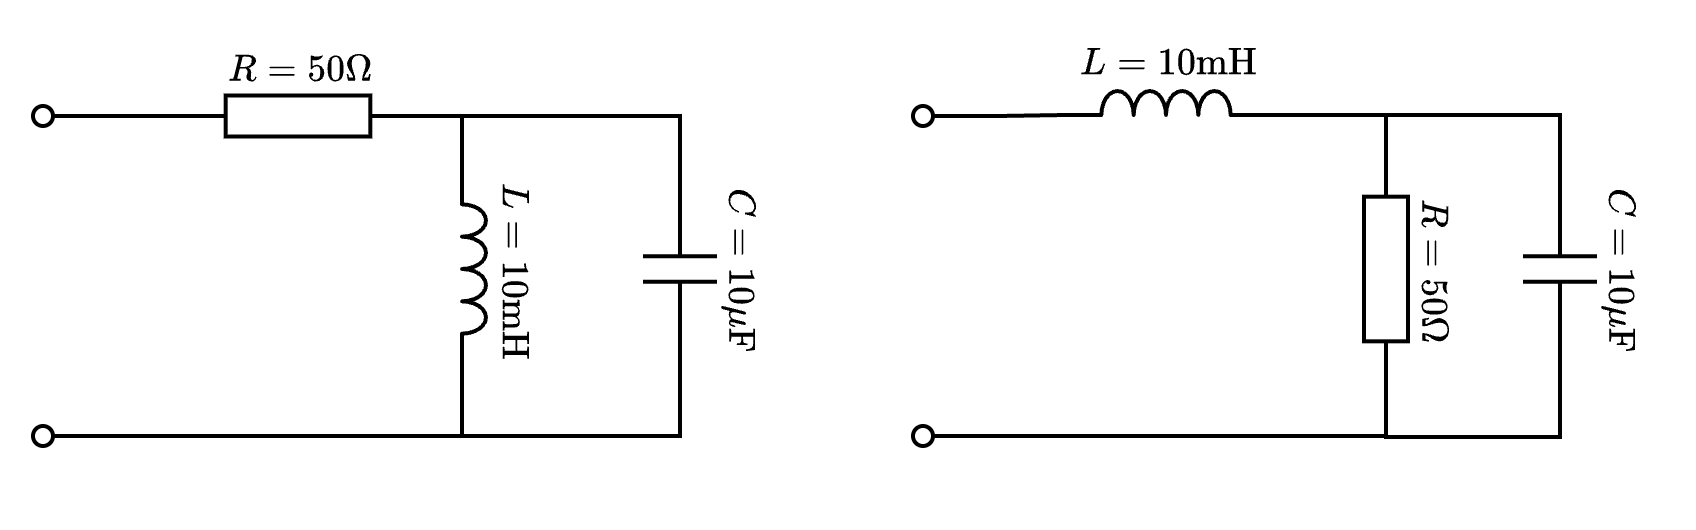
\includegraphics[width=6.77083in,height=\textheight,keepaspectratio]{media/ejercicio4.png}

}

\caption{Ejercicios Impedancia}

\end{figure}%

\begin{itemize}
\tightlist
\item
  \emph{Solución 1:}
  \(\vec{Z} = 50 + 68,21 \mathrm{j} \ \Omega = 84,57 \phase{53,76^\circ} \ \Omega\).
\item
  \emph{Solución 2:}
  \(\vec{Z} = 19,40 + 0,78 \mathrm{j} \ \Omega = 19,42 \phase{2,3^\circ} \ \Omega\).
\end{itemize}

\textbf{5. Análisis Fasorial}

\vspace{-1em}

Dibuja el diagrama fasorial correspondiente al circuito de la figura y
calcula la tensión en la bobina.

\begin{figure}[H]

{\centering 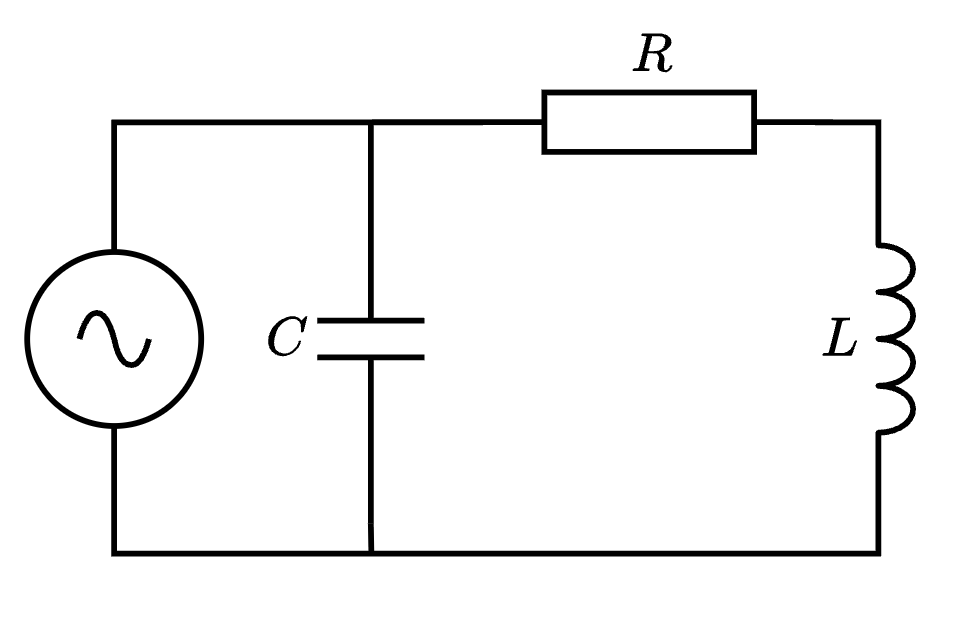
\includegraphics[width=3.64583in,height=\textheight,keepaspectratio]{media/ejercicio5.png}

}

\caption{Ejercicios Fasorial}

\end{figure}%

\vspace{-1em}

\begin{itemize}
\tightlist
\item
  \emph{Datos:} \(R = 2 \ \Omega\), \(L = \frac{1}{50\pi} \ \text{H}\),
  \(C = \frac{1}{300\pi} \ \text{F}\), \(U = 10 \ \text{V}\) y
  \(f = 50 \ \text{Hz}\).
\item
  \emph{Solución:} \(\vec{U}_L = 5 \sqrt{2} \mathrm{j} \ \text{V}\)
  \emph{(tomando como referencia de fases la intensidad de la
  resistencia)}.
\end{itemize}

\textbf{6. Desfase en Serie RL}

\vspace{-1em}

En un circuito \(R-L\) serie hay un desfase de \(30^\circ\) entre la
tensión de alimentación y la tensión de la resistencia. Calcula el valor
de la inductancia que consigue dicho desfase. Dibuja el triángulo de
impedancias.

\vspace{-1em}

\begin{itemize}
\tightlist
\item
  \emph{Datos:} \(f = 50 \ \text{Hz}\), \(U = 30 \ \text{V}\),
  \(R = 5 \ \Omega\).
\item
  \emph{Solución:} \(L=9,188 \text{mH}\).
\end{itemize}

\textbf{7. Circuito RC Serie}

\vspace{-1em}

En un circuito la tensión en una resistencia vale \(15 \ \text{V}\) y la
intensidad que circula por un condensador colocado en serie con ella es
de \(0,5 \ \text{A}\). Si la tensión de la fuente es de
\(20 \ \text{V}\) y la frecuencia de \(30 \ \text{Hz}\), calcula:

\vspace{-1em}

\begin{enumerate}
\def\labelenumi{\alph{enumi})}
\tightlist
\item
  El valor de la resistencia.
\item
  La reactancia capacitiva.
\item
  El triángulo de impedancias.
\end{enumerate}

\begin{itemize}
\tightlist
\item
  \emph{Solución:}
  \(a) \ R=30 \ \Omega ;b) \ X_c=26,46 \ \Omega; c) \ \vec{Z} = 40 \phase{-41,41^\circ} \ \Omega\).
\end{itemize}

\textbf{8. Corrientes en Paralelo}

\vspace{-1em}

En el circuito de la figura, que funciona a una frecuencia de
\(50 \ \text{Hz}\), se obtienen las siguientes medidas con los aparatos
de medida:

\vspace{-1em}

\begin{itemize}
\tightlist
\item
  \(A_1=13 \ \text{A}\).
\item
  \(A_2=11 \ \text{A}\).
\item
  \(V_1=220 \ \text{V}\).
\end{itemize}

\begin{figure}[H]

{\centering 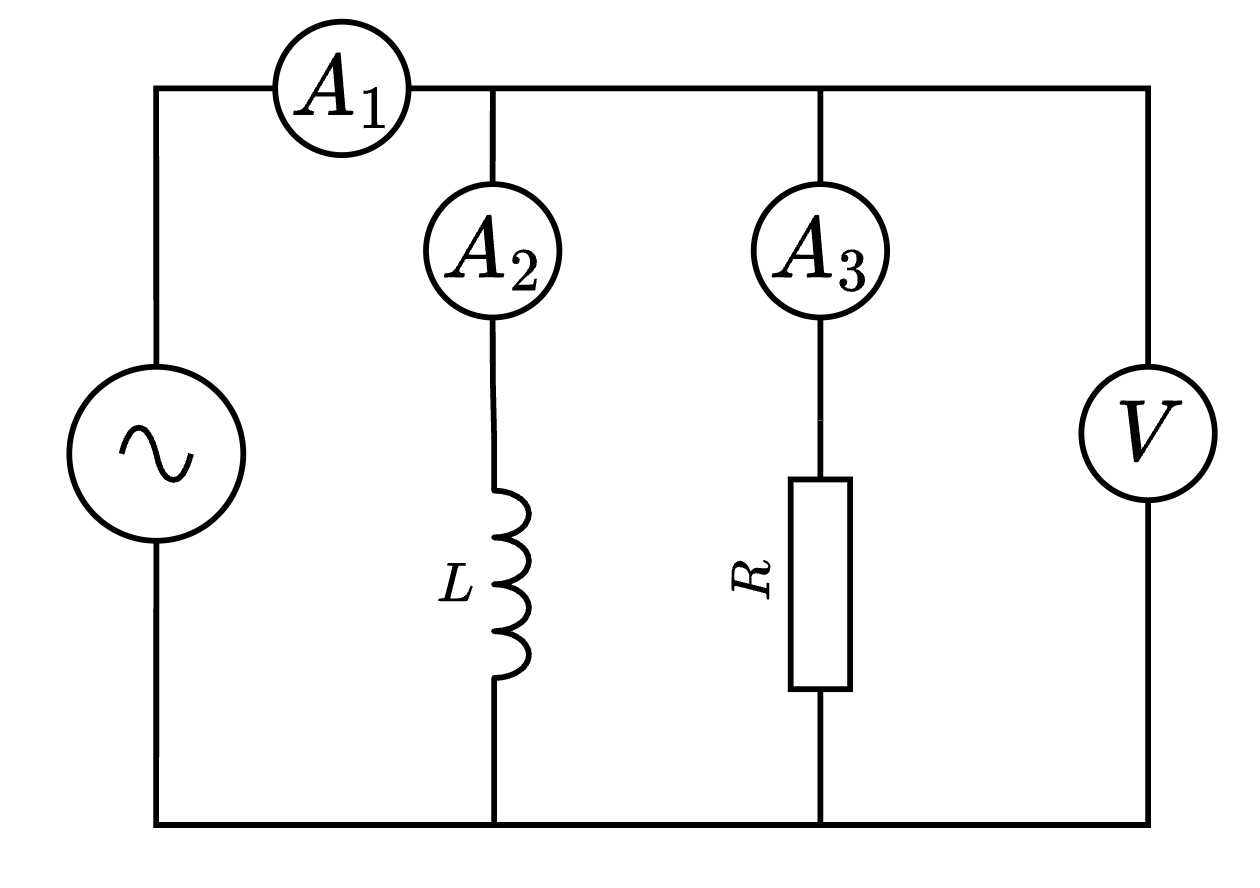
\includegraphics[width=3.64583in,height=\textheight,keepaspectratio]{media/ejercicio8.png}

}

\caption{Ejercicios Paralelo}

\end{figure}%

Determina:

\vspace{-1em}

\begin{enumerate}
\def\labelenumi{\alph{enumi})}
\tightlist
\item
  La representación vectorial de las corrientes y la medida del
  amperímetro \(A_3\).
\item
  El valor de \(R\).
\item
  El valor de \(L\).
\end{enumerate}

\begin{itemize}
\tightlist
\item
  \emph{Solución:}
  \(a) \ 6,93 \ \text{A} ;b) \ 31,75 \ \Omega; c) \ 63,66 \ \text{mH}\).
\end{itemize}

\end{tcolorbox}

\bookmarksetup{startatroot}

\chapter{Circuitos RLC}\label{circuitos-rlc}

\section{Circuito RLC serie}\label{circuito-rlc-serie}

Uno de los circuitos típicos en corriente alterna es el circuito RLC
serie que se muestra en la siguiente figura:

\begin{figure}

\begin{minipage}{0.70\linewidth}

\begin{figure}[H]

{\centering 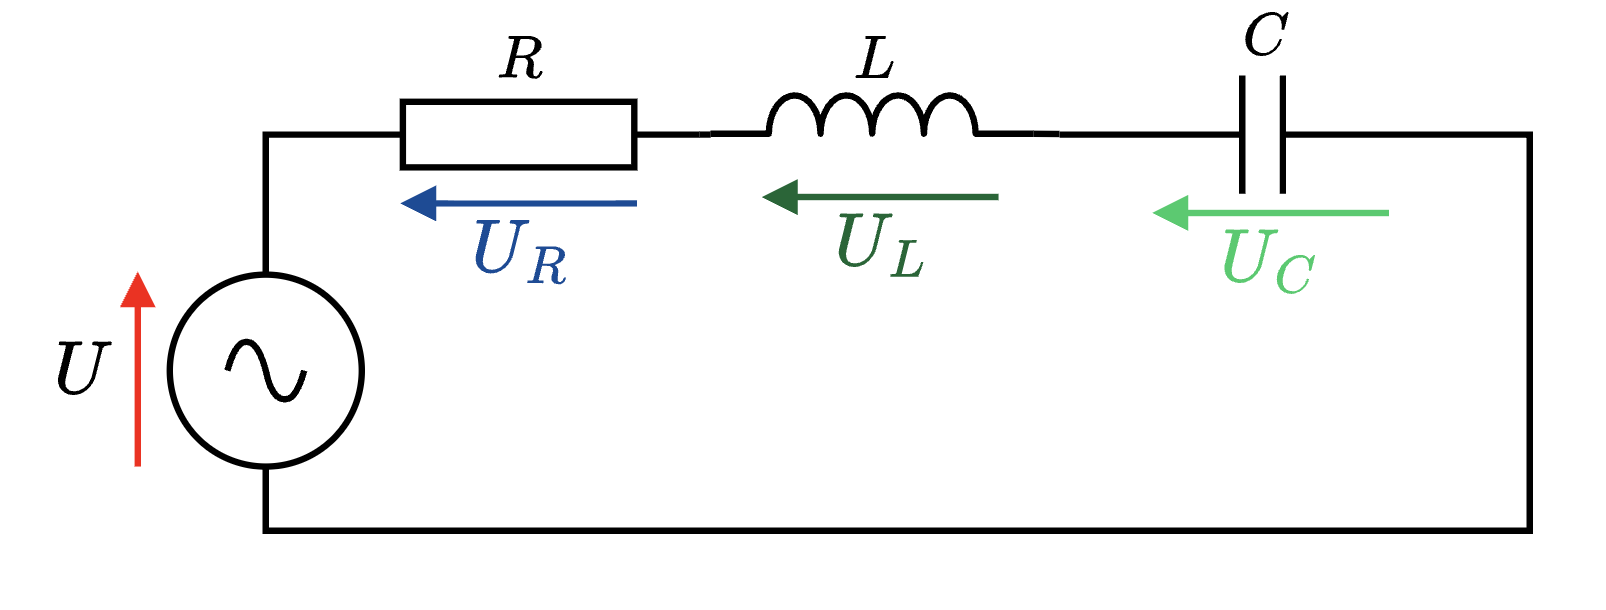
\includegraphics[width=1\linewidth,height=\textheight,keepaspectratio]{media/esquema_rlc_serie.png}

}

\subcaption{Esquema RLC}

\end{figure}%

\end{minipage}%
%
\begin{minipage}{0.30\linewidth}

\begin{figure}[H]

{\centering 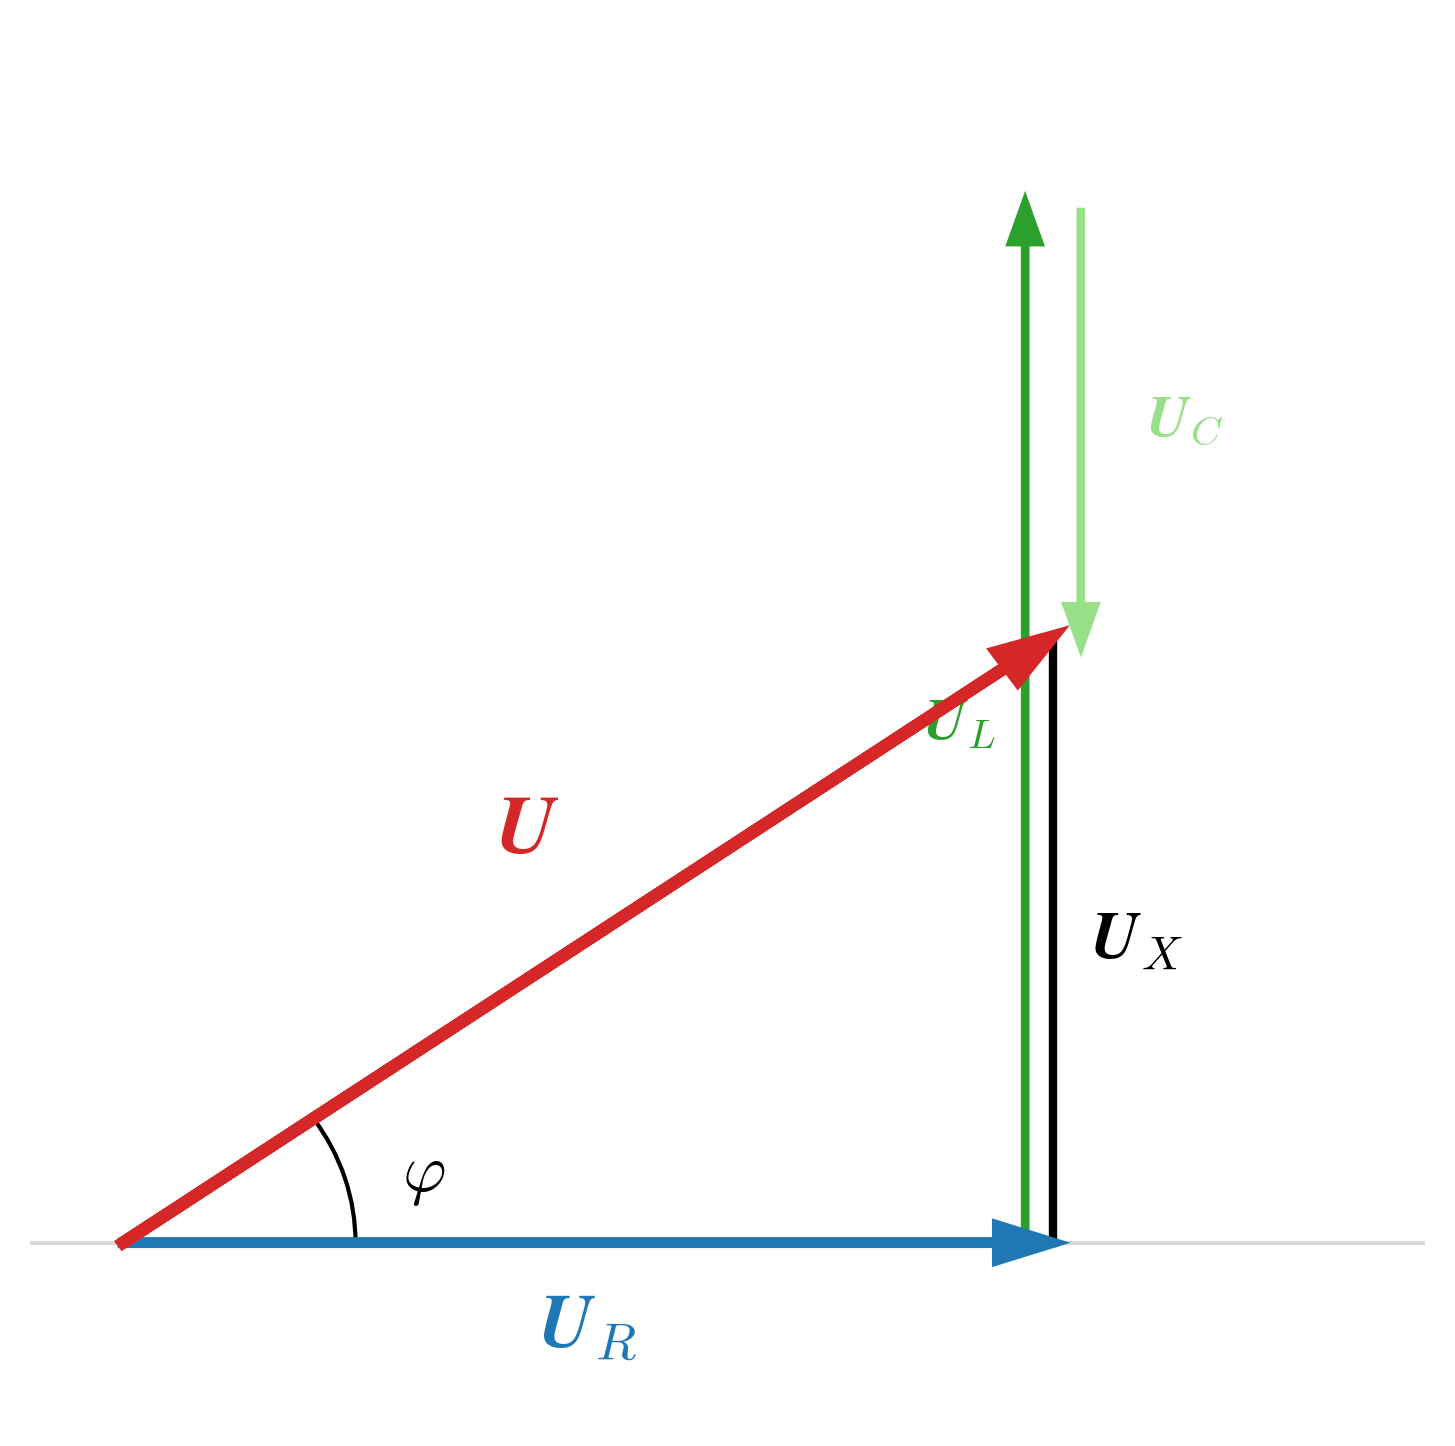
\includegraphics[width=1\linewidth,height=\textheight,keepaspectratio]{media/tensiones_rlc_fiel.png}

}

\subcaption{Diagrama Vectorial de Tensiones}

\end{figure}%

\end{minipage}%

\end{figure}%

Tomando como \textbf{referencia de ángulos la intensidad}
\((\varphi_I=0^\circ, \vec{I}=I\angle 0^\circ)\) la tensión en cada
elemento es:

\[
\begin{aligned}
\vec{U}_R &= R \cdot \vec{I} \\
\vec{U}_L &= \mathrm{j} \cdot X_L \cdot \vec{I} \\
\vec{U}_C &= -\mathrm{j} \cdot X_C \cdot \vec{I}
\end{aligned}
\]

La tensión total \(\vec{U}\) es la suma vectorial de las tensiones
parciales; así tenemos:

\[
\begin{aligned}
\vec{U} &= \vec{U}_R + \vec{U}_L + \vec{U}_C = \\
&= R \cdot \vec{I} + \mathrm{j} \cdot X_L \cdot \vec{I} - \mathrm{j} \cdot X_C \cdot \vec{I} = \\
&= [R + \mathrm{j} \cdot (X_L - X_C)] \cdot \vec{I}
\end{aligned}
\]

La expresión anterior se puede poner como:

\[
\vec{U} = (R + \mathrm{j} \cdot X) \cdot \vec{I} = \vec{Z} \cdot \vec{I}
\]

La impedancia del circuito es:

\[
\vec{Z} = R + \mathrm{j} \cdot (X_L - X_C) = R + \mathrm{j} \cdot \left( \omega \cdot L - \frac{1}{\omega \cdot C} \right)
\]

Expresado en coordenadas polares resulta:

\[
\vec{Z} = |\vec{Z}| \angle \varphi = 
\left\{
\begin{aligned}
|\vec{Z}| &= \sqrt{R^2 + X^2} = \sqrt{R^2 + (X_L - X_C)^2} = \sqrt{R^2 + \left( \omega \cdot L - \frac{1}{\omega \cdot C} \right)^2} \\[2ex]
\varphi &= \arctan\left( \frac{X}{R} \right) = \arctan\left( \frac{X_L - X_C}{R} \right) = \arctan\left( \frac{\omega \cdot L - \frac{1}{\omega \cdot C}}{R} \right)
\end{aligned}
\right.
\]

\begin{figure}[H]

{\centering 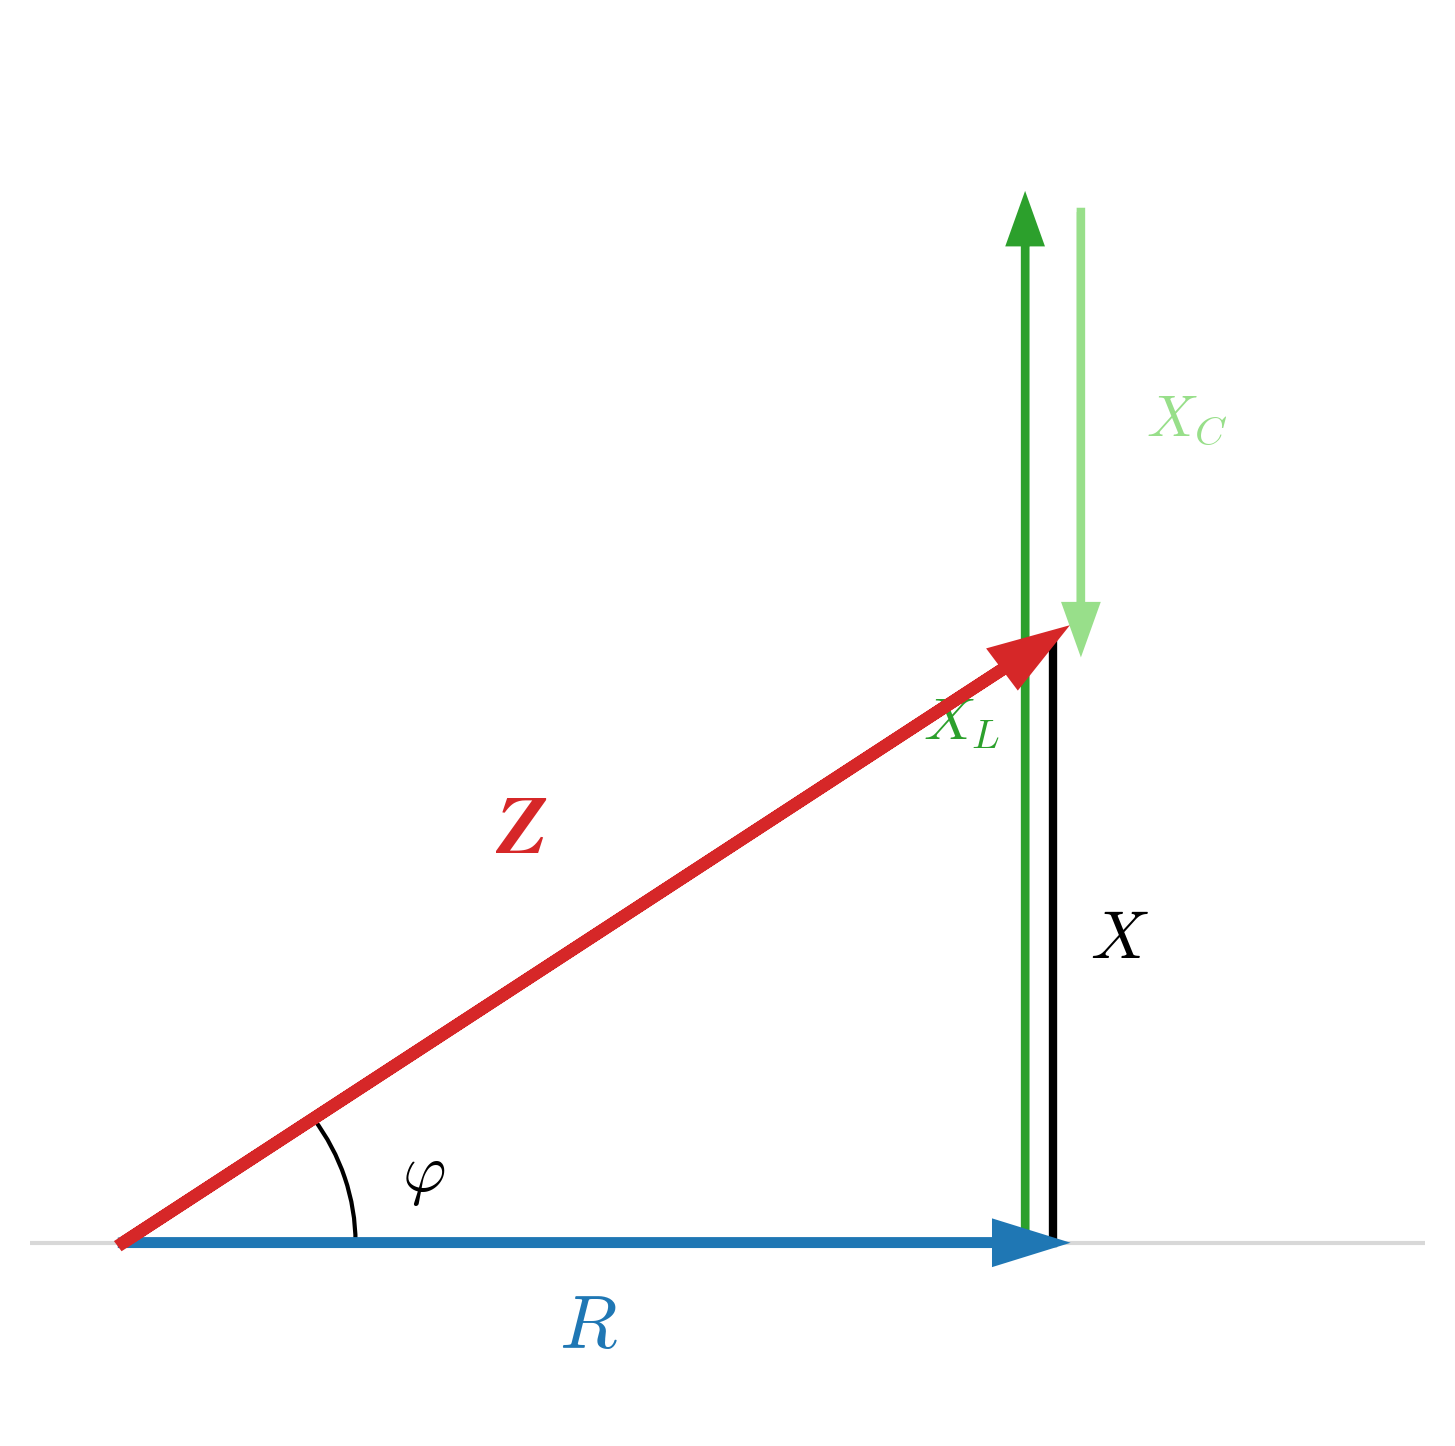
\includegraphics[width=0.5\linewidth,height=\textheight,keepaspectratio]{media/impedancias_rlc_fiel.png}

}

\caption{Triángulo de Impedancias}

\end{figure}%

\begin{tcolorbox}[enhanced jigsaw, breakable, colback=white, left=2mm, leftrule=.75mm, rightrule=.15mm, toprule=.15mm, colframe=quarto-callout-important-color-frame, arc=.35mm, bottomrule=.15mm, opacityback=0]

\vspace{-3mm}\textbf{💡 Ejercicio Resuelto: Análisis RLC Serie}\vspace{3mm}

\textbf{Enunciado:} En un circuito RLC serie con \(R=20\ \Omega\),
\(L=100/\pi\ \text{mH}\) y \(C=1/2\pi\ \text{mF}\), funcionando a una
frecuencia de \(50\ \text{Hz}\), calcula:\\
\strut ~~~\textbf{a)} La impedancia total (módulo y argumento).\\
\strut ~~~\textbf{b)} La intensidad que circula si la tensión es de
\(230\ \text{V}\).\\
\strut ~~~\textbf{c)} Diagrama fasorial.

\begin{center}\rule{0.5\linewidth}{0.5pt}\end{center}

\textbf{Solución:}

\textbf{1. Cálculo de Reactancias:} Primero obtenemos los valores
óhmicos de la bobina y el condensador a \(f=50\text{Hz}\).

\[
\begin{aligned}
X_L &= \omega \cdot L = 2\pi \cdot 50 \cdot \frac{100}{\pi} \cdot 10^{-3} = 10\ \Omega \\
X_C &= \frac{1}{\omega \cdot C} = \frac{1}{2\pi \cdot 50 \cdot \frac{1}{2\pi} \cdot 10^{-3}} = \frac{1}{50 \cdot 10^{-3}} = 20\ \Omega
\end{aligned}
\]

\textbf{2. Cálculo de la Impedancia (\(\vec{Z}\)):} Como \(X_C > X_L\),
el circuito será capacitivo. Restamos las reactancias
(\(X = X_L - X_C = 10 - 20 = -10\ \Omega\)).

\begin{itemize}
\item
  \textbf{Forma Binómica:}
  \[\vec{Z} = R + \mathrm{j}(X_L - X_C) = 20 - \mathrm{j}10\ \Omega\]
\item
  \textbf{Forma Polar:} Pasamos a polar calculando módulo y argumento:
  \[|\vec{Z}| = \sqrt{20^2 + (-10)^2} = 22,36\ \Omega\]
  \[\varphi = \arctan\left(\frac{-10}{20}\right) = -26,56^\circ\]
\end{itemize}

\begin{figure}[H]

\begin{minipage}{0.50\linewidth}
\textbf{Resultado Impedancia:}
\[\vec{Z} = 22,36 \phase{-26,56^\circ}\ \Omega\]Como \(\varphi < 0\),
confirmamos que la tensión está \textbf{retrasada} respecto a la
intensidad (comportamiento capacitivo).\end{minipage}%
%
\begin{minipage}{0.50\linewidth}

\begin{figure}[H]

{\centering 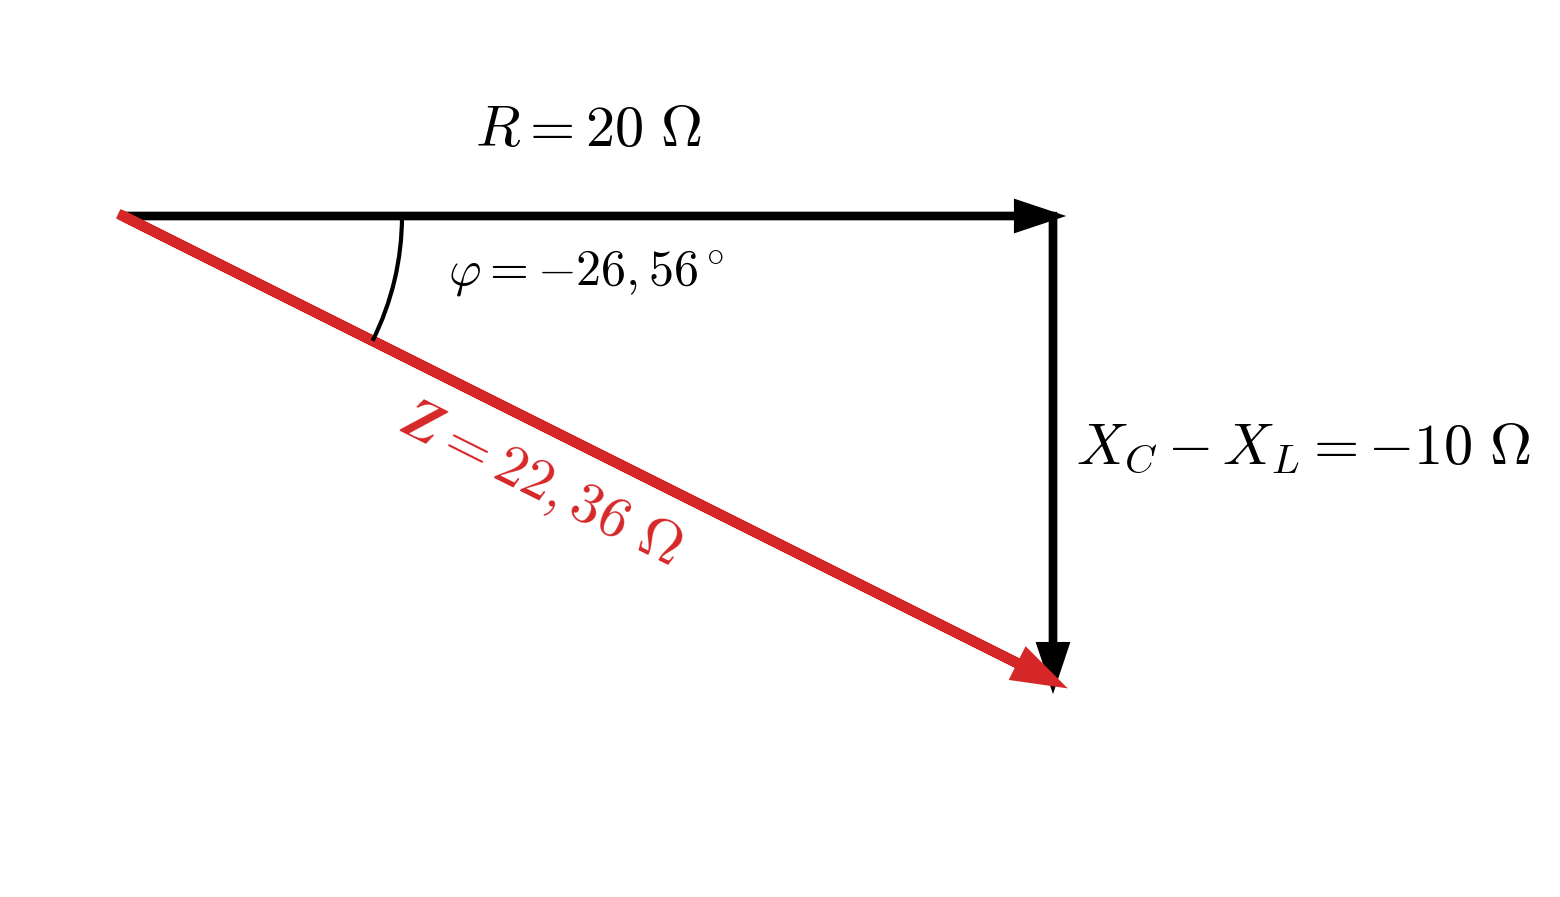
\includegraphics[width=0.9\linewidth,height=\textheight,keepaspectratio]{media/triangulo_ejemplo_serie.png}

}

\subcaption{Triángulo de Impedancias}

\end{figure}%

\end{minipage}%

\end{figure}%

\textbf{3. Cálculo de la Intensidad (\(\vec{I}\)):} Aplicamos la Ley de
Ohm generalizada. Tomamos la tensión como referencia de fase
(\(0^\circ\)):

\[
\vec{I} = \frac{\vec{U}}{\vec{Z}} = \frac{230 \phase{0^\circ}}{22,36 \phase{-26,56^\circ}} = 10,29 \phase{0^\circ - (-26,56^\circ)}\ \text{A}
\]

\[\boxed{\vec{I} = 10,29 \phase{26,56^\circ}\ \text{A}}\]

\begin{center}\rule{0.5\linewidth}{0.5pt}\end{center}

\textbf{4. Diagrama Fasorial U-I (Apartado c):} Representamos los
fasores resultantes.

\begin{figure}[H]

\begin{minipage}{0.50\linewidth}

\begin{itemize}
\tightlist
\item
  \textbf{Tensión (\(\vec{U}\)):} En el eje real (\(0^\circ\)).
\item
  \textbf{Intensidad (\(\vec{I}\)):} Girada \(+26,56^\circ\).
\end{itemize}

Como se observa en el diagrama, el fasor de intensidad \(\vec{I}\)
(azul) está \textbf{adelantado} respecto al fasor de tensión \(\vec{U}\)
(rojo) un ángulo \(\varphi = 26,56^\circ\).Esto confirma el
comportamiento \textbf{capacitivo} global del circuito.\end{minipage}%
%
\begin{minipage}{0.50\linewidth}

\begin{figure}[H]

{\centering 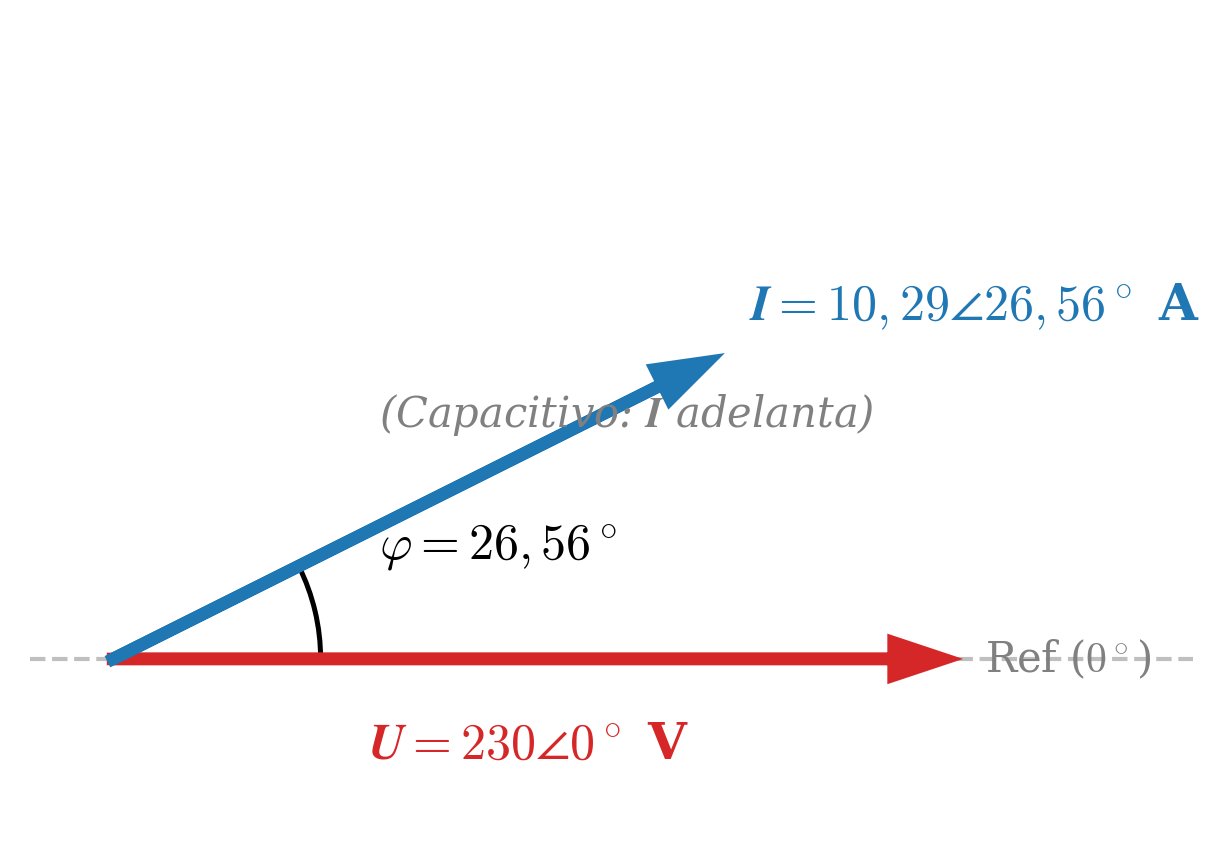
\includegraphics[width=0.9\linewidth,height=\textheight,keepaspectratio]{media/fasores_ui_ejercicio.png}

}

\subcaption{Diagrama Fasorial U-I}

\end{figure}%

\end{minipage}%

\end{figure}%

\end{tcolorbox}

\section{Circuito RLC Paralelo}\label{circuito-rlc-paralelo}

De forma análoga al circuito serie, el circuito RLC paralelo es el
estándar para analizar componentes conectados a la misma tensión.

\begin{figure}

\begin{minipage}{0.60\linewidth}

\begin{figure}[H]

{\centering 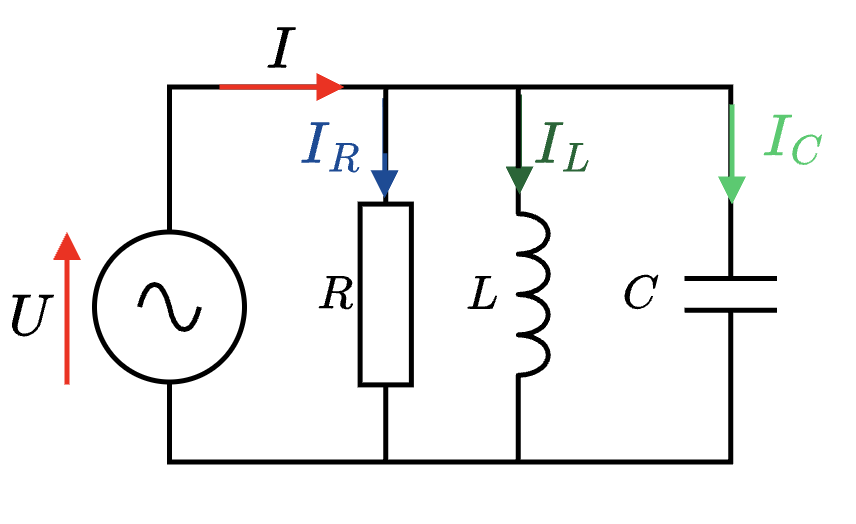
\includegraphics[width=1\linewidth,height=\textheight,keepaspectratio]{media/esquema_rlc_paralelo.png}

}

\subcaption{Esquema RLC Paralelo}

\end{figure}%

\end{minipage}%
%
\begin{minipage}{0.40\linewidth}

\begin{figure}[H]

{\centering 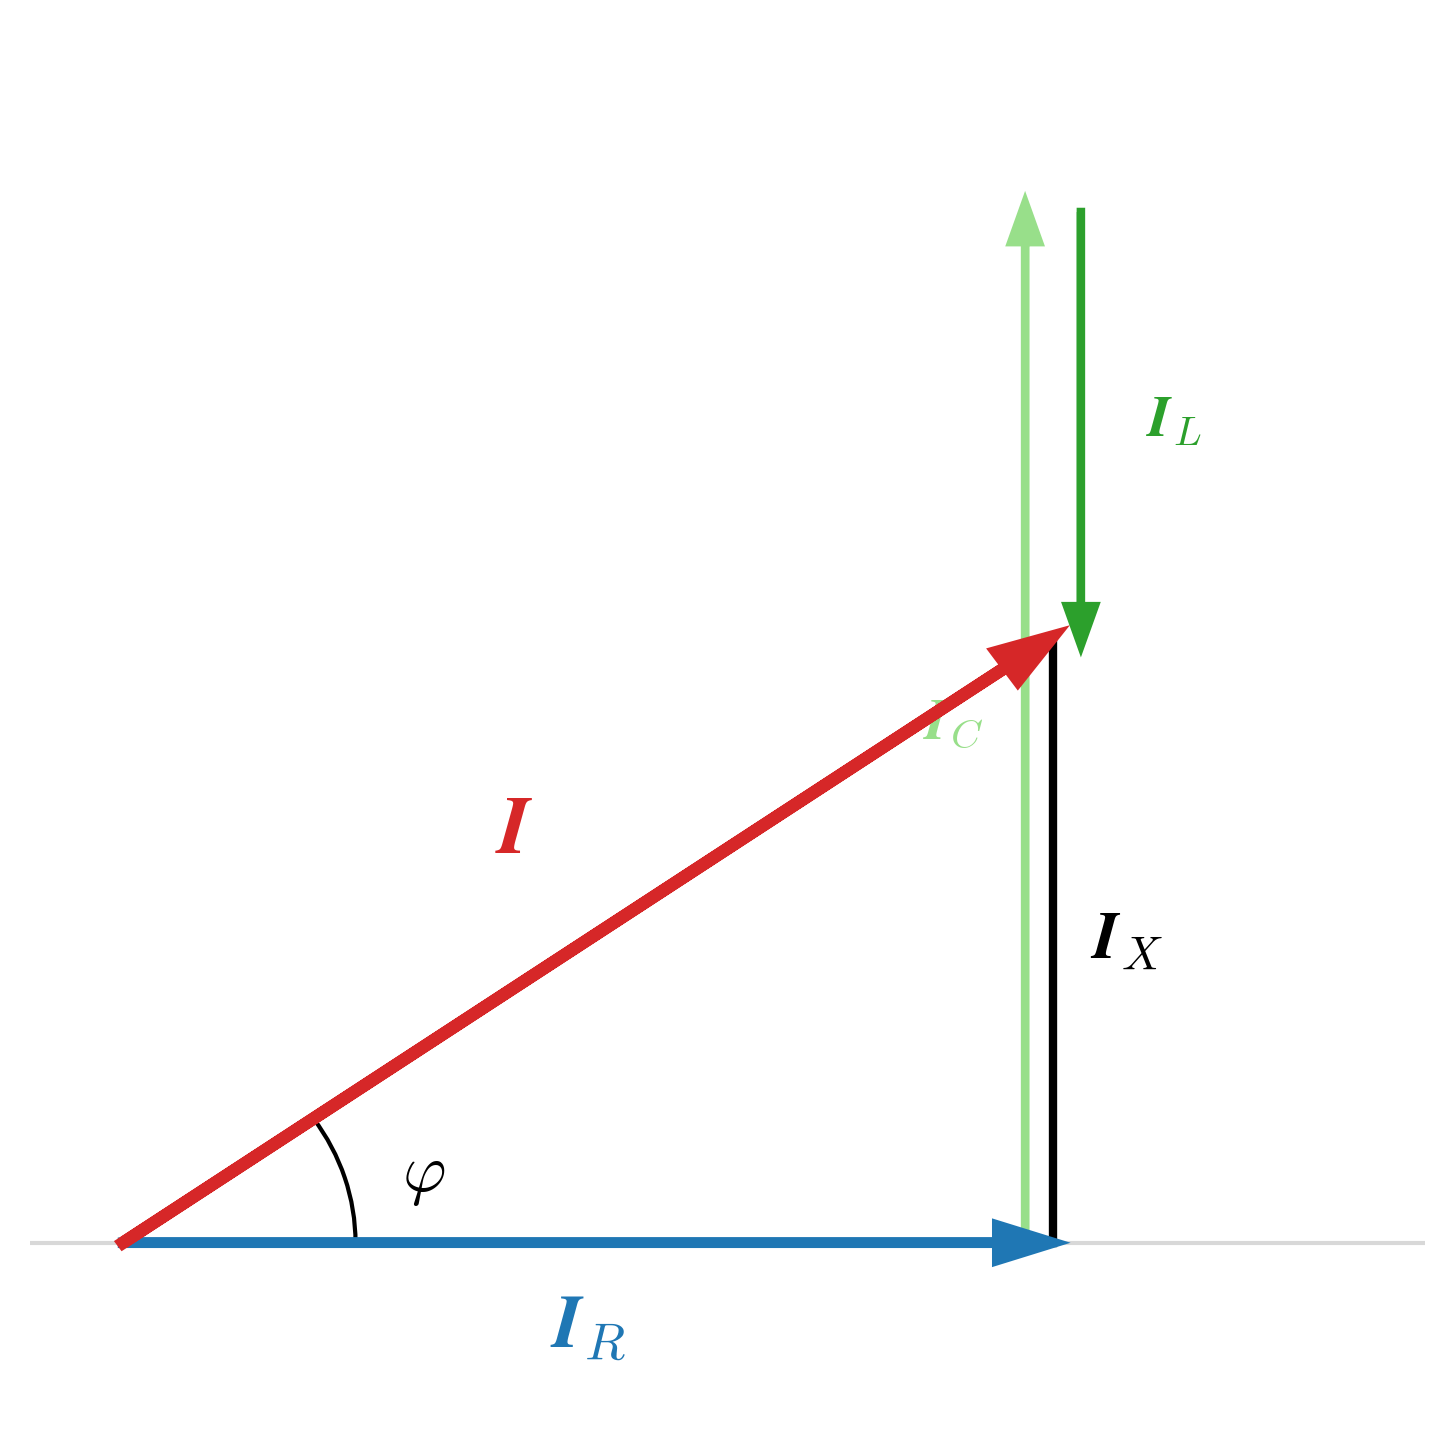
\includegraphics[width=1\linewidth,height=\textheight,keepaspectratio]{media/corrientes_paralelo_fiel.png}

}

\subcaption{Diagrama Vectorial de Corrientes}

\end{figure}%

\end{minipage}%

\end{figure}%

Tomando como referencia de ángulos la tensión común
\((\varphi_U=0^\circ, \vec{U}=U\angle 0^\circ)\) la corriente en cada
rama es:

\[
\begin{aligned}
\vec{I}_R &= \frac{\vec{U}}{R} = G \cdot \vec{U} \\
\vec{I}_C &= \frac{\vec{U}}{-\mathrm{j}X_C} = \mathrm{j} \cdot \frac{1}{X_C} \cdot \vec{U} \\
\vec{I}_L &= \frac{\vec{U}}{\mathrm{j}X_L} = -\mathrm{j} \cdot \frac{1}{X_L} \cdot \vec{U}
\end{aligned}
\]

La corriente total \(\vec{I}\) es la suma vectorial de las corrientes de
rama (Ley de Kirchhoff de los nodos); así tenemos:

\[
\begin{aligned}
\vec{I} &= \vec{I}_R + \vec{I}_C + \vec{I}_L= \\
&= \frac{1}{R} \cdot \vec{U} + \mathrm{j} \frac{1}{X_C} \cdot \vec{U} - \mathrm{j} \frac{1}{X_L} \cdot \vec{U}= \\
&= \left[ \frac{1}{R} + \mathrm{j} \cdot \left(\frac{1}{X_C} - \frac{1}{X_L}\right) \right] \cdot \vec{U}
\end{aligned}
\]

\begin{tcolorbox}[enhanced jigsaw, breakable, colback=white, left=2mm, leftrule=.75mm, rightrule=.15mm, toprule=.15mm, colframe=quarto-callout-warning-color-frame, arc=.35mm, bottomrule=.15mm, opacityback=0]

\vspace{-3mm}\textbf{📘 Diccionario: Admitancia, Conductancia y Susceptancia}\vspace{3mm}

En circuitos paralelo, es más cómodo trabajar con la facilidad que
ofrecen los elementos al paso de la corriente (inverso de la oposición).
Todas se miden en \textbf{Siemens (S)}.

\begin{enumerate}
\def\labelenumi{\arabic{enumi}.}
\item
  \textbf{Admitancia (\(\vec{Y}\)):} Es la inversa de la Impedancia.
  Representa la facilidad total al paso de la corriente alterna.
  \[\vec{Y} = \frac{1}{\vec{Z}}\]
\item
  \textbf{Conductancia (\(G\)):} Es la inversa de la Resistencia.
  Representa la parte real de la admitancia. \[G = \frac{1}{R}\]
\item
  \textbf{Susceptancia (\(B\)):} Es la inversa de la Reactancia.
  Representa la parte imaginaria.

  \vspace{-1em}

  \begin{itemize}
  \tightlist
  \item
    \textbf{Susceptancia Capacitiva (\(B_C\)):}
    \(B_C = \frac{1}{X_C} = \omega \cdot C\)
  \item
    \textbf{Susceptancia Inductiva (\(B_L\)):}
    \(B_L = \frac{1}{X_L} = \frac{1}{\omega \cdot L}\)
  \end{itemize}
\end{enumerate}

⚠️ \textbf{¡Cuidado con los signos!} Al trabajar con admitancias, los
signos imaginarios se invierten respecto a las impedancias (porque
\(1/\mathrm{j} = -\mathrm{j}\)):

\vspace{-1em}

\begin{itemize}
\tightlist
\item
  El \textbf{Condensador} aporta susceptancia \textbf{positiva}
  (\(+\mathrm{j}B_C\)).
\item
  La \textbf{Bobina} aporta susceptancia \textbf{negativa}
  (\(-\mathrm{j}B_L\)).
\end{itemize}

Si necesitas la Impedancia equivalente total, simplemente invierte el
resultado final: \(\vec{Z}_{T} = 1 / \vec{Y}_{T}\).

\end{tcolorbox}

\vspace{1em}

La expresión anterior se puede poner como la Ley de Ohm generalizada
\(\vec{I} = \vec{Y} \cdot \vec{U}\), donde el término entre corchetes es
la \textbf{Admitancia (\(\vec{Y}\))}.

\[
\vec{I} = (G + \mathrm{j} \cdot B) \cdot \vec{U} = \vec{Y} \cdot \vec{U}
\]

La \textbf{admitancia} del circuito (inversa de la impedancia,
\(\vec{Y} = 1/\vec{Z}\)) es:

\[
\vec{Y} = \frac{1}{R} + \mathrm{j} \cdot \left( \omega \cdot C - \frac{1}{\omega \cdot L} \right)
\]

En forma polar sería:

\[
\vec{Y} = |\vec{Y}| \angle \varphi = 
\left\{
\begin{aligned}
|\vec{Y}| &= \sqrt{G^2 + B^2} = \sqrt{\left(\frac{1}{R}\right)^2 + (B_C - B_L)^2} = \sqrt{\left(\frac{1}{R}\right)^2 + \left( \omega \cdot C - \frac{1}{\omega \cdot L} \right)^2} \\[2ex]
\varphi &= \arctan\left( \frac{B}{G} \right) = \arctan\left( \frac{B_C - B_L}{G} \right) = \arctan\left( \frac{\omega \cdot C - \frac{1}{\omega \cdot L}}{1/R} \right)
\end{aligned}
\right.
\]

\begin{figure}[H]

{\centering 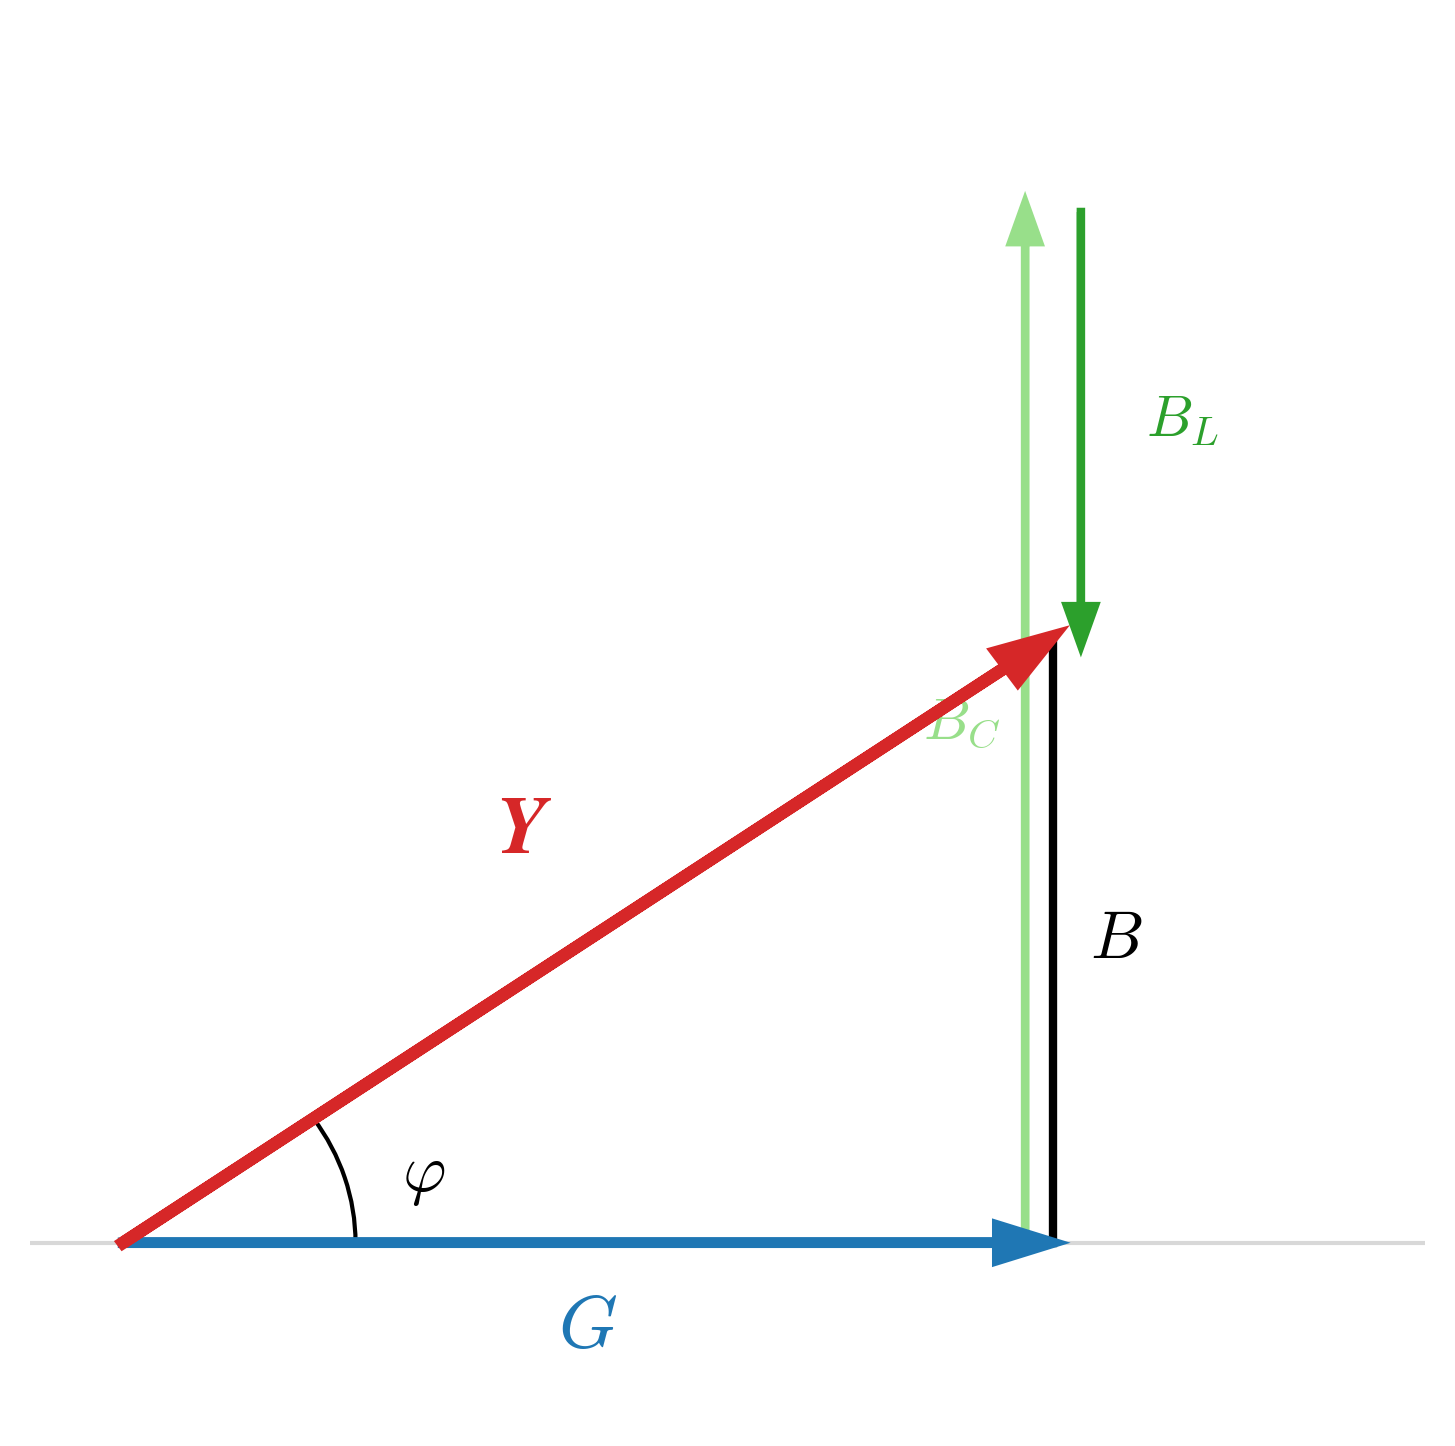
\includegraphics[width=0.5\linewidth,height=\textheight,keepaspectratio]{media/admitancias_paralelo_fiel.png}

}

\caption{Triángulo de Admitancias}

\end{figure}%

\begin{tcolorbox}[enhanced jigsaw, breakable, colback=white, left=2mm, leftrule=.75mm, rightrule=.15mm, toprule=.15mm, colframe=quarto-callout-important-color-frame, arc=.35mm, bottomrule=.15mm, opacityback=0]

\vspace{-3mm}\textbf{💡 Ejercicio Resuelto: Análisis RLC Paralelo}\vspace{3mm}

\textbf{Enunciado:} En un circuito RLC paralelo con \(R=20\ \Omega\),
\(L=100/\pi\ \text{mH}\) y \(C=1/2\pi\ \text{mF}\), funcionando a
\(f=50\ \text{Hz}\) y conectado a \(U=230\ \text{V}\), calcula:\\
\strut ~~~~\textbf{a)} Admitancia e Impedancia equivalente.\\
\strut ~~~~\textbf{b)} Intensidad por cada elemento.\\
\strut ~~~~\textbf{c)} Diagrama fasorial de la tensión y las
corrientes.\\

\begin{center}\rule{0.5\linewidth}{0.5pt}\end{center}

\textbf{Solución:}

\textbf{Paso previo:} Calculamos conductancias y susceptancias. \[
\begin{aligned}
G &= \frac{1}{R} = \frac{1}{20} = 0,05\ \text{S} \\
X_L &= 10\ \Omega \Rightarrow B_L = \frac{1}{X_L} = 0,1\ \text{S} \\
X_C &= 20\ \Omega \Rightarrow B_C = \frac{1}{X_C} = 0,05\ \text{S}
\end{aligned}
\]

\textbf{a) Admitancia (\(\vec{Y}\)) e Impedancia (\(\vec{Z}\)):} \[
\vec{Y} = G + \mathrm{j}(B_C - B_L) = 0,05 + \mathrm{j}(0,05 - 0,1) = 0,05 - \mathrm{j}0,05\ \text{S}
\] En polar:
\(\vec{Y} = \sqrt{0,05^2 + 0,05^2} \angle \arctan(-1) = 0,0707 \angle -45^\circ\ \text{S}\).

La impedancia es la inversa: \[
\vec{Z} = \frac{1}{\vec{Y}} = \frac{1}{0,0707 \angle -45^\circ} = 14,14 \angle 45^\circ\ \Omega \quad (= 10 + \mathrm{j}10\ \Omega)
\]

\textbf{b) Corrientes de Rama:} Tomando
\(\vec{U} = 230 \angle 0^\circ\ \text{V}\): \[
\begin{aligned}
\vec{I}_R &= \vec{U} \cdot G = 230 \cdot 0,05 = 11,5 \angle 0^\circ\ \text{A} (=11,5\ \text{A}) \\
\vec{I}_L &= \vec{U} \cdot (-\mathrm{j}B_L) = 230 \cdot 0,1 \angle -90^\circ = 23 \angle -90^\circ\ \text{A} (=-23\mathrm{j}\ \text{A}) \\
\vec{I}_C &= \vec{U} \cdot (\mathrm{j}B_C) = 230 \cdot 0,05 \angle 90^\circ = 11,5 \angle 90^\circ\ \text{A} (=11,5\mathrm{j}\ \text{A})
\end{aligned}
\]

\textbf{Cálculo de la Total:}
\(\vec{I}_T = \vec{I}_R + \vec{I}_L + \vec{I}_C = 11,5 + \mathrm{j}(11,5 - 23) = 11,5 - \mathrm{j}11,5\ \text{A}\).
\[|\vec{I}_T| = 16,26\ \text{A} \quad ; \quad \varphi = -45^\circ\]

\begin{figure}[H]

\begin{minipage}{0.50\linewidth}
\textbf{Resultado:} \[\vec{I}_T = 16,26 \phase{-45^\circ}\ \text{A}\] El
circuito es \textbf{Inductivo} (la corriente total retrasa
\(45^\circ\)).\end{minipage}%
%
\begin{minipage}{0.50\linewidth}

\begin{figure}[H]

{\centering 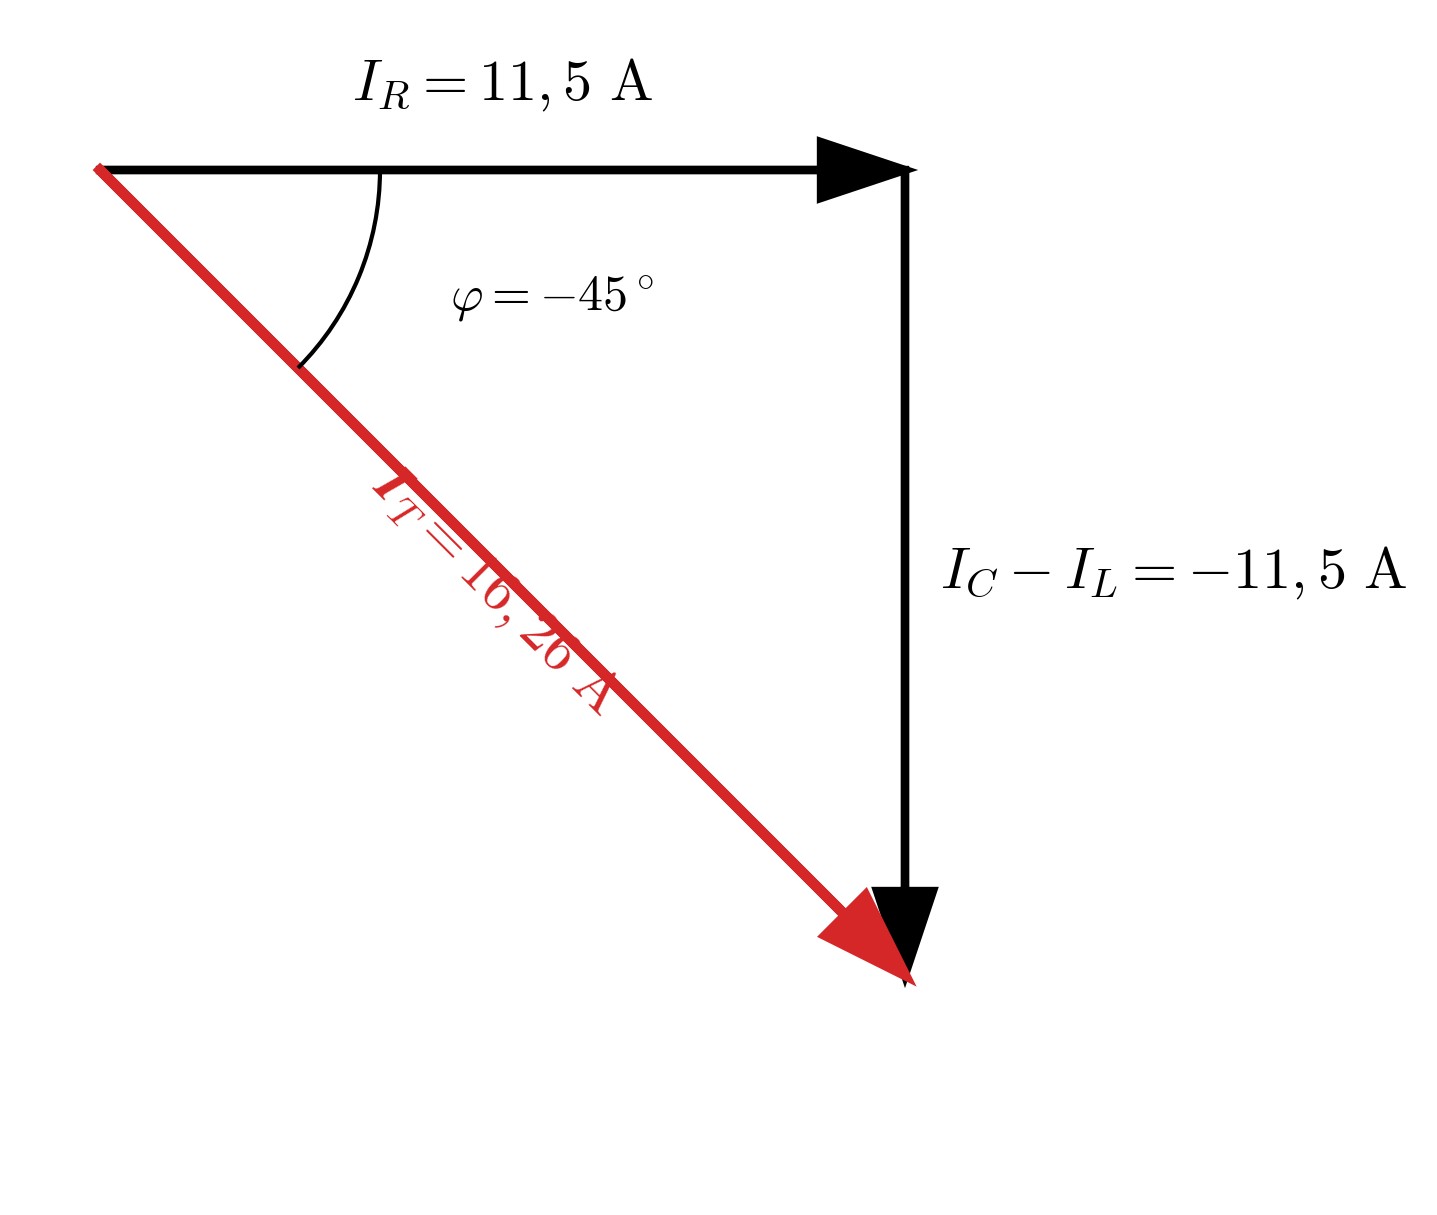
\includegraphics[width=0.9\linewidth,height=\textheight,keepaspectratio]{media/triangulo_paralelo_real.png}

}

\subcaption{Triángulo de Corrientes}

\end{figure}%

\end{minipage}%

\end{figure}%

\begin{center}\rule{0.5\linewidth}{0.5pt}\end{center}

\textbf{c) Diagrama Fasorial:} Representamos la tensión y las
corrientes. Observa que \(\vec{I}_L\) (23 A) es mayor que \(\vec{I}_C\)
(11,5 A), ``tirando'' de la resultante hacia abajo.

\begin{figure}[H]

\begin{minipage}{0.50\linewidth}

\begin{itemize}
\tightlist
\item
  \textbf{Tensión (\(\vec{U}\)):} Referencia horizontal.
\item
  \textbf{Corrientes:} La suma vectorial da una resultante en el cuarto
  cuadrante.
\end{itemize}

Se ve claramente que la intensidad total \(\vec{I}_T\) (flecha roja)
está retrasada respecto a la tensión, confirmando el carácter
inductivo.\end{minipage}%
%
\begin{minipage}{0.50\linewidth}

\begin{figure}[H]

{\centering 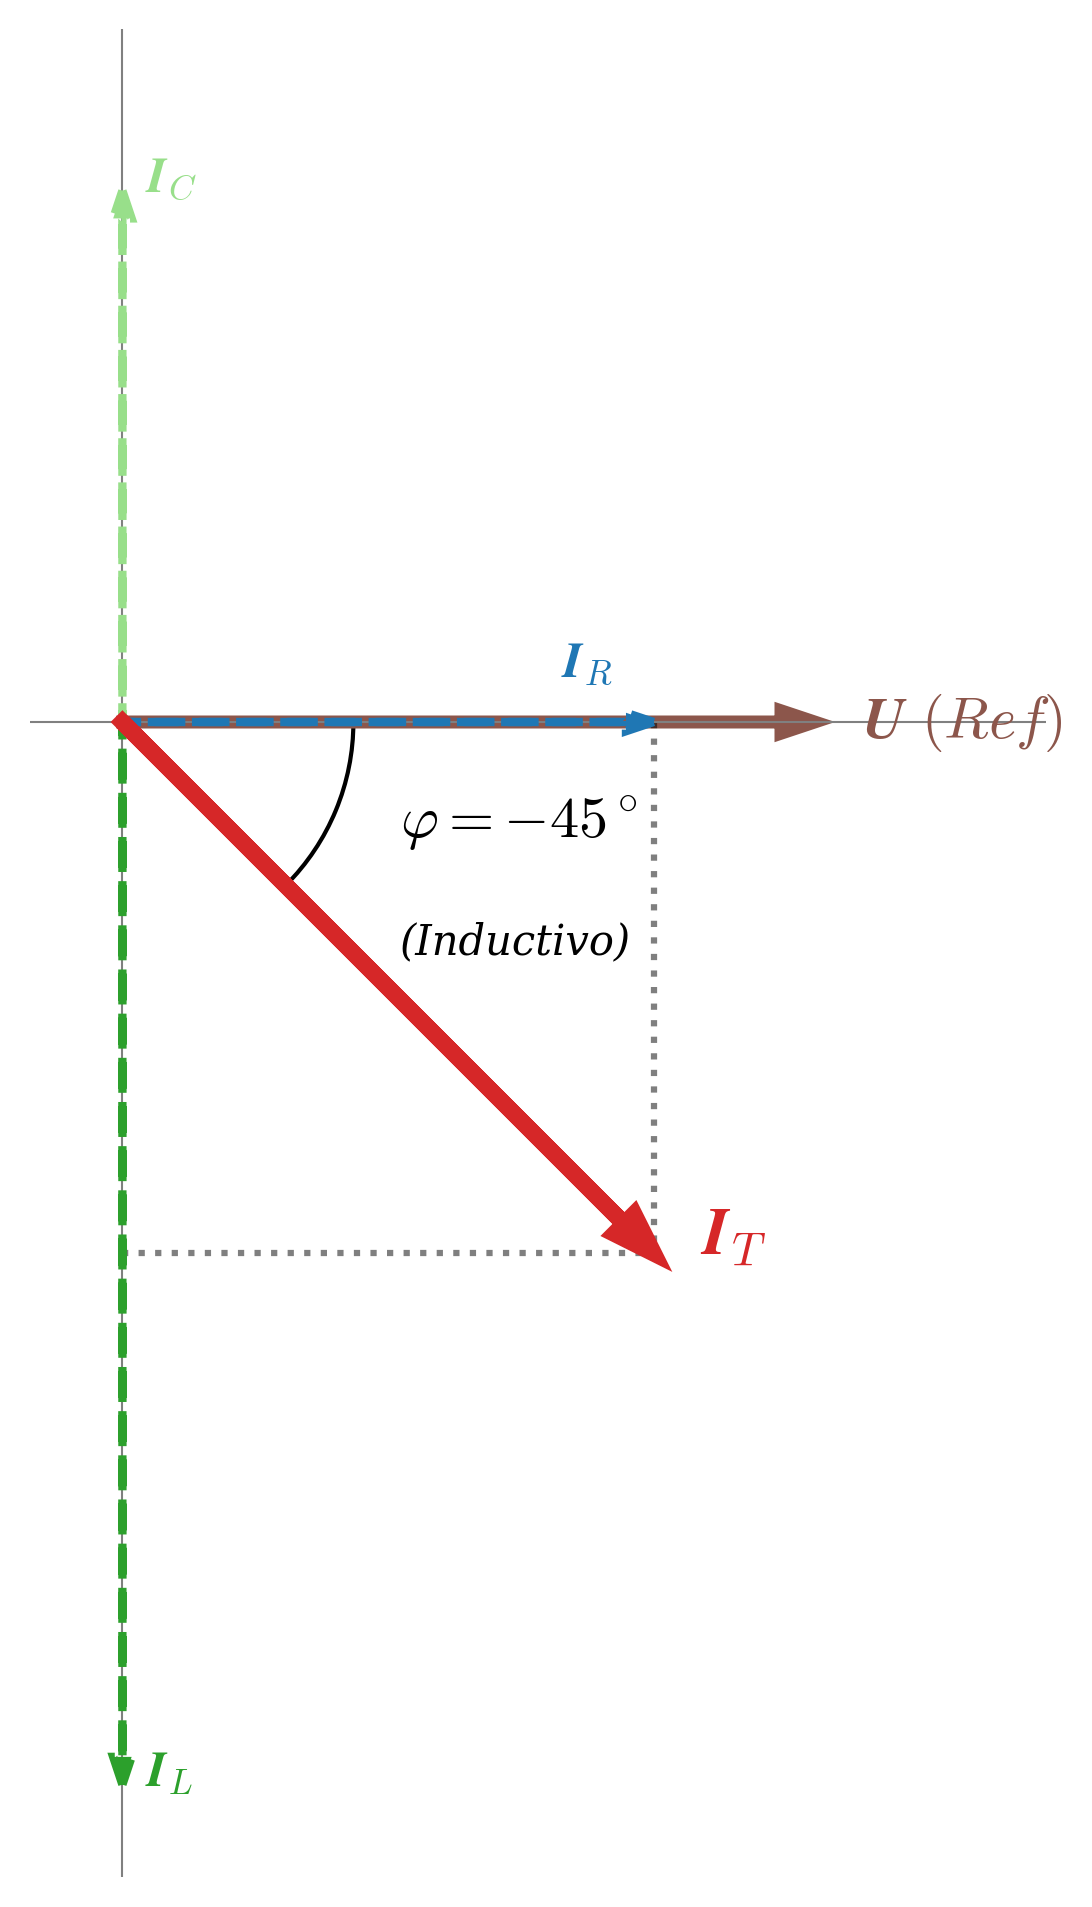
\includegraphics[width=0.95\linewidth,height=\textheight,keepaspectratio]{media/fasorial_paralelo_real.png}

}

\subcaption{Diagrama Fasorial Completo}

\end{figure}%

\end{minipage}%

\end{figure}%

\end{tcolorbox}

\section{Frecuencia de Resonancia}\label{frecuencia-de-resonancia}

En los circuitos RLC, existe una frecuencia específica muy especial en
la que los efectos de la bobina y el condensador se anulan mutuamente.
Este fenómeno se conoce como \textbf{Resonancia}.

\subsection{Condición de Resonancia}\label{condiciuxf3n-de-resonancia}

La resonancia ocurre cuando la Reactancia Inductiva iguala en magnitud a
la Reactancia Capacitiva.

\[
X_L = X_C
\]

A partir de esta igualdad, podemos deducir el valor de la frecuencia de
resonancia (\(f_0\)):

\[
\begin{aligned}
\omega_0 \cdot L &= \frac{1}{\omega_0 \cdot C} \\[1ex]
\omega_0^2 &= \frac{1}{L \cdot C} \\[1ex]
\omega_0 &= \frac{1}{\sqrt{L \cdot C}}
\end{aligned}
\]

Como \(\omega = 2 \pi f\), despejamos la frecuencia:

\begin{tcolorbox}[enhanced jigsaw, breakable, colback=white, left=2mm, leftrule=.75mm, rightrule=.15mm, toprule=.15mm, colframe=quarto-callout-warning-color-frame, arc=.35mm, bottomrule=.15mm, opacityback=0]

\vspace{-3mm}\textbf{🚩 Fórmula de Thomson (Frecuencia de Resonancia)}\vspace{3mm}

\[
f_0 = \frac{1}{2 \cdot \pi \cdot \sqrt{L \cdot C}}
\]

\end{tcolorbox}

\subsection{Comportamiento del
Circuito}\label{comportamiento-del-circuito}

A esta frecuencia \(f_0\), el circuito se comporta como si fuera
\textbf{Puramente Resistivo}, ya que las partes imaginarias se cancelan
(\(\mathrm{j}X_L - \mathrm{j}X_C = 0\)).

\begin{figure}

\begin{minipage}{0.50\linewidth}

\begin{figure}[H]

{\centering 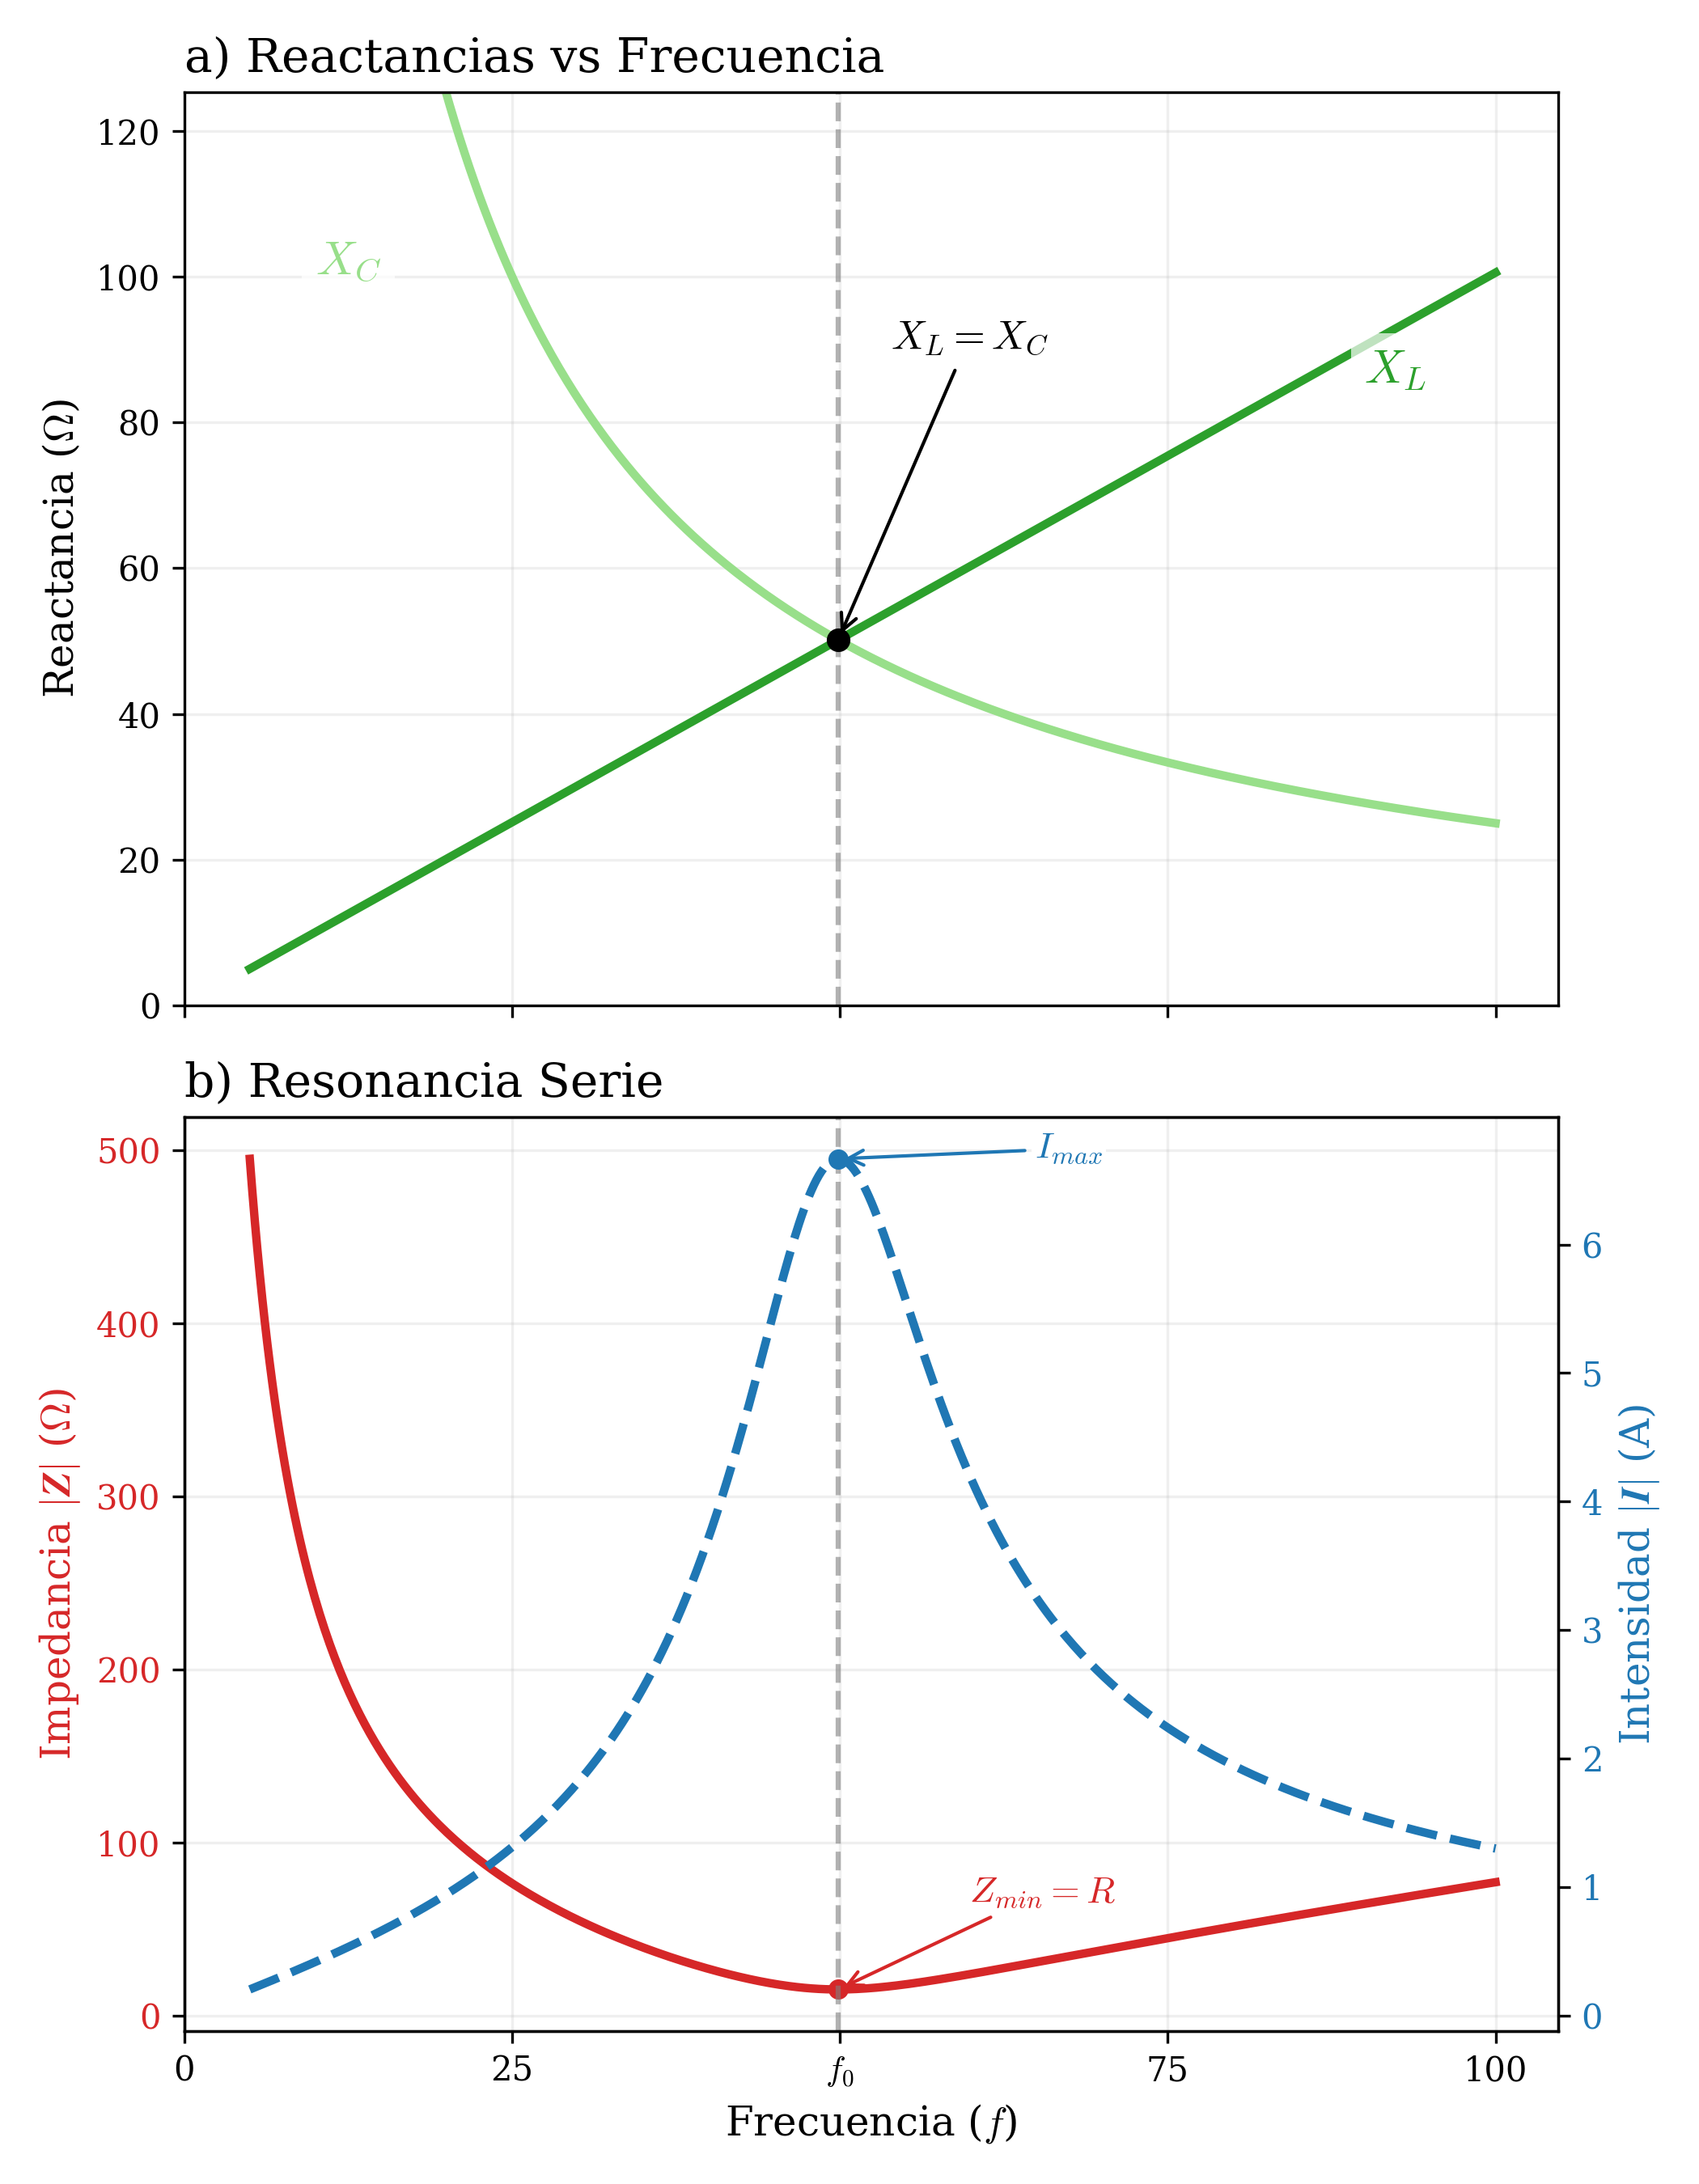
\includegraphics[width=1\linewidth,height=\textheight,keepaspectratio]{media/resonancia_graficas.png}

}

\subcaption{Comportamiento en Frecuencia}

\end{figure}%

\end{minipage}%
%
\begin{minipage}{0.50\linewidth}
\textbf{Análisis Gráfico:}

\begin{enumerate}
\def\labelenumi{\arabic{enumi}.}
\item
  \textbf{Bajas Frecuencias (\(f < f_0\)):} El condensador domina
  (\(X_C\) es muy grande). El circuito es \textbf{Capacitivo}.
\item
  \textbf{Punto de Resonancia (\(f = f_0\)):} \(X_L\) y \(X_C\) se
  cruzan. La impedancia es puramente resistiva (\(\vec{Z}=R\)).
\item
  \textbf{Altas Frecuencias (\(f > f_0\)):} La bobina domina (\(X_L\)
  crece). El circuito se vuelve \textbf{Inductivo}.
\end{enumerate}

\end{minipage}%

\end{figure}%

\subsection{Diferencias: Resonancia Serie vs
Paralelo}\label{diferencias-resonancia-serie-vs-paralelo}

Aunque la frecuencia \(f_0\) se calcula igual para ambos, las
consecuencias físicas son opuestas:

\begin{longtable}[]{@{}
  >{\raggedright\arraybackslash}p{(\linewidth - 4\tabcolsep) * \real{0.3333}}
  >{\raggedright\arraybackslash}p{(\linewidth - 4\tabcolsep) * \real{0.3333}}
  >{\raggedright\arraybackslash}p{(\linewidth - 4\tabcolsep) * \real{0.3333}}@{}}
\caption{Comparativa de efectos de la
resonancia.}\label{tbl-resonancia-comparativa}\tabularnewline
\toprule\noalign{}
\begin{minipage}[b]{\linewidth}\raggedright
Característica
\end{minipage} & \begin{minipage}[b]{\linewidth}\raggedright
\textbf{Resonancia SERIE}
\end{minipage} & \begin{minipage}[b]{\linewidth}\raggedright
\textbf{Resonancia PARALELO}
\end{minipage} \\
\midrule\noalign{}
\endfirsthead
\toprule\noalign{}
\begin{minipage}[b]{\linewidth}\raggedright
Característica
\end{minipage} & \begin{minipage}[b]{\linewidth}\raggedright
\textbf{Resonancia SERIE}
\end{minipage} & \begin{minipage}[b]{\linewidth}\raggedright
\textbf{Resonancia PARALELO}
\end{minipage} \\
\midrule\noalign{}
\endhead
\bottomrule\noalign{}
\endlastfoot
\textbf{Impedancia Total} & \textbf{Mínima} (\(\vec{Z} = R\)) &
\textbf{Máxima} (\(\vec{Z} \to \infty\) idealmente) \\
\textbf{Intensidad de Fuente} & \textbf{Máxima} & \textbf{Mínima} \\
\textbf{Peligro / Efecto} & \textbf{Sobretensiones:}En \(L\) y \(C\)
puede haber voltajes mucho mayores que la fuente. &
\textbf{Sobrecorrientes:}Entre \(L\) y \(C\) circula una corriente
interna muy alta (corriente oscilante). \\
\end{longtable}

\begin{tcolorbox}[enhanced jigsaw, breakable, colback=white, left=2mm, leftrule=.75mm, rightrule=.15mm, toprule=.15mm, colframe=quarto-callout-tip-color-frame, arc=.35mm, bottomrule=.15mm, opacityback=0]

\vspace{-3mm}\textbf{⚠️ Precaución en el Laboratorio}\vspace{3mm}

En resonancia serie, aunque la fuente sea de solo 10V, ¡la tensión en la
bobina o el condensador podría alcanzar cientos de voltios!
(\(U_L = Q \cdot U_{\text{fuente}}\)). Hay que tener cuidado manipulando
los circuitos cerca de \(f_0\).

\end{tcolorbox}

\begin{center}\rule{0.5\linewidth}{0.5pt}\end{center}

\begin{tcolorbox}[enhanced jigsaw, breakable, colback=white, left=2mm, leftrule=.75mm, rightrule=.15mm, toprule=.15mm, colframe=quarto-callout-important-color-frame, arc=.35mm, bottomrule=.15mm, opacityback=0]

\vspace{-3mm}\textbf{📝 Ejercicios de Repaso}\vspace{3mm}

Resuelve los siguientes circuitos considerando una frecuencia de red de
\textbf{50 Hz} (\(\omega = 100\pi \ \text{rad/s}\)).

\subsection*{Circuitos Serie}\label{circuitos-serie}
\addcontentsline{toc}{subsection}{Circuitos Serie}

\textbf{1. RLC con Impedancia Exacta}\\
Disponemos de una resistencia \(R=8 \ \Omega\), una bobina ideal de
inductancia \(L=40/\pi \ \text{mH}\) y un condensador de capacidad
\(C=1000/\pi \ \mu\text{F}\) conectados en serie. Se aplica una tensión
de \(200 \ \text{V}\).\\
\strut ~~~\textbf{a)} Calcula la reactancia inductiva (\(X_L\)) y
capacitiva (\(X_C\)).\\
\strut ~~~\textbf{b)} Determina la impedancia total en forma binómica y
polar.\\
\strut ~~~\textbf{c)} Calcula la intensidad que circula por el
circuito.\\
\strut ~~~\emph{Soluciones:} \(X_L=4 \ \Omega, X_C=10 \ \Omega\);
\(\vec{Z}=8-\mathrm{j}6 = 10 \phase{-36,87^\circ} \ \Omega\);
\(I=20 \ \text{A}\).

\textbf{2. La Bobina Real}\\
Una bobina real tiene una resistencia interna de \(30 \ \Omega\) y una
inductancia de \(127,3 \ \text{mH}\) (\(L \approx 0,4/\pi \ \text{H}\)).
Se conecta en serie con un condensador de \(C=50 \ \mu\text{F}\). El
conjunto se alimenta a \(230 \ \text{V}\).\\
\strut ~~~\textbf{a)} Calcula la impedancia compleja de la bobina
(\(\vec{Z}_{\text{bobina}}\)) y la del condensador (\(\vec{Z}_C\)).\\
\strut ~~~\textbf{b)} Obtén la impedancia total del circuito y la
intensidad.\\
\strut ~~~\textbf{c)} ¿El circuito se comporta globalmente como
inductivo o capacitivo?\\
\strut ~~~\emph{Soluciones:}
\(\vec{Z}_{\text{bobina}}=30+\mathrm{j}40 \ \Omega\);
\(\vec{Z}_C=-\mathrm{j}63,66 \ \Omega\);
\(\vec{Z}_T=30-\mathrm{j}23,66 \ \Omega\); \(I=6,02 \ \text{A}\);
Capacitivo.

\begin{center}\rule{0.5\linewidth}{0.5pt}\end{center}

\subsection*{Circuitos Paralelo}\label{circuitos-paralelo}
\addcontentsline{toc}{subsection}{Circuitos Paralelo}

\textbf{3. Corrientes de Rama}\\
Se conectan en paralelo una resistencia \(R=20 \ \Omega\), una bobina
\(L=100/\pi \ \text{mH}\) y un condensador \(C=500/\pi \ \mu\text{F}\) a
una fuente de \(100 \ \text{V}\).\\
\strut ~~~\textbf{a)} Calcula la corriente que circula por cada rama
(\(\vec{I}_R, \vec{I}_L, \vec{I}_C\)).\\
\strut ~~~\textbf{b)} Calcula la corriente total mediante suma
vectorial. Dibuja el diagrama fasorial.\\
\strut ~~~\emph{Soluciones:} \(I_R=5 \ \text{A} \phase{0^\circ}\);
\(I_L=10 \ \text{A} \phase{-90^\circ}\);
\(I_C=5 \ \text{A} \phase{90^\circ}\);
\(I_{total}=7,07 \ \text{A} \phase{-45^\circ}\).

\textbf{4. Cálculo por Admitancias}\\
Un circuito paralelo está formado por una conductancia
\(G=0,03 \ \text{S}\), una susceptancia inductiva
\(B_L=0,04 \ \text{S}\) y un condensador cuya reactancia es
\(X_C=20 \ \Omega\). La tensión aplicada es de \(200 \ \text{V}\).\\
\strut ~~~\textbf{a)} Determina la susceptancia del condensador
(\(B_C\)) en Siemens.\\
\strut ~~~\textbf{b)} Calcula la admitancia total \(\vec{Y}\) en forma
binómica y polar.\\
\strut ~~~\textbf{c)} Determina la intensidad total y la impedancia
equivalente del conjunto.\\
\strut ~~~\emph{Soluciones:} \(B_C=0,05 \ \text{S}\);
\(\vec{Y}=0,03+\mathrm{j}0,01 \ \text{S} = 0,0316 \phase{18,43^\circ} \ \text{S}\);
\(I=6,32 \ \text{A}\);
\(\vec{Z}_{eq}=31,62 \phase{-18,43^\circ} \ \Omega\).

\end{tcolorbox}

\bookmarksetup{startatroot}

\chapter{Potencia en Corriente
Alterna}\label{potencia-en-corriente-alterna}

En corriente continua, la potencia era simple: \(P = V \cdot I\). Sin
embargo, en corriente alterna, el desfase entre tensión e intensidad
hace que aparezcan \textbf{tres formas de entender la energía}.

\section{Conceptos Fundamentales}\label{conceptos-fundamentales-1}

Cuando aplicamos una tensión alterna a una carga, la energía fluye.
Dependiendo de si la carga almacena energía (bobinas/condensadores) o la
consume (resistencias), definimos:

\subsection*{\texorpdfstring{A. Potencia Activa
(\(P\))}{A. Potencia Activa (P)}}\label{a.-potencia-activa-p}
\addcontentsline{toc}{subsection}{A. Potencia Activa (\(P\))}

Es la \textbf{potencia útil}, la que realmente realiza un trabajo
(calor, luz, movimiento). Se disipa en las resistencias.

\vspace{-1em}

\begin{itemize}
\tightlist
\item
  \textbf{Símbolo:} \(P\)
\item
  \textbf{Unidad:} Vatio (\textbf{W})
\item
  \textbf{Fórmula:} \(P = U \cdot I \cdot \cos \varphi\)
\end{itemize}

\subsection*{\texorpdfstring{B. Potencia Reactiva
(\(Q\))}{B. Potencia Reactiva (Q)}}\label{b.-potencia-reactiva-q}
\addcontentsline{toc}{subsection}{B. Potencia Reactiva (\(Q\))}

Es una potencia ``de ida y vuelta''. No realiza trabajo útil;
simplemente se dedica a crear y destruir campos magnéticos (bobinas) y
eléctricos (condensadores). La fuente la entrega y el componente la
devuelve 50 veces por segundo.

\vspace{-1em}

\begin{itemize}
\tightlist
\item
  \textbf{Símbolo:} \(Q\)
\item
  \textbf{Unidad:} Voltamperio reactivo (\textbf{var})
\item
  \textbf{Fórmula:} \(Q = U \cdot I \cdot \sen \varphi\)
\end{itemize}

\begin{tcolorbox}[enhanced jigsaw, breakable, colback=white, left=2mm, leftrule=.75mm, rightrule=.15mm, toprule=.15mm, colframe=quarto-callout-warning-color-frame, arc=.35mm, bottomrule=.15mm, opacityback=0]

\vspace{-3mm}\textbf{⚠️ Ojo con las unidades: ¿var o VAr?}\vspace{3mm}

Existe una discrepancia habitual entre la norma técnica y la costumbre
académica:

\begin{enumerate}
\def\labelenumi{\arabic{enumi}.}
\tightlist
\item
  \textbf{La Norma (Lo correcto):} La Comisión Electrotécnica
  Internacional (IEC) establece que el símbolo único y oficial es
  \textbf{var} (en minúsculas). Así lo usaremos en estos apuntes.
\item
  \textbf{La Costumbre (Lo habitual):} En muchos libros de texto,
  exámenes de Selectividad y placas de características industriales,
  verás escrito \textbf{VAr} o \textbf{VAR} (usando mayúsculas por venir
  de Voltio y Amperio).
\end{enumerate}

\textbf{Consejo para el examen:} Aunque \texttt{var} es lo técnicamente
perfecto, si en el enunciado de tu examen aparece \texttt{VAr}, puedes
usar esa notación sin miedo. Ambas se aceptan universalmente en el
ámbito de la ingeniería práctica.

\end{tcolorbox}

\subsection*{\texorpdfstring{C. Potencia Aparente
(\(S\))}{C. Potencia Aparente (S)}}\label{c.-potencia-aparente-s}
\addcontentsline{toc}{subsection}{C. Potencia Aparente (\(S\))}

Es la potencia total que debe suministrar la fuente (o la que dimensiona
los cables y transformadores). Es la suma vectorial de las anteriores.

\vspace{-1em}

\begin{itemize}
\tightlist
\item
  \textbf{Símbolo:} \(S\) (o \(|\vec{S}|\))
\item
  \textbf{Unidad:} Voltamperio (\textbf{VA})
\item
  \textbf{Fórmula:} \(S = U \cdot I = \sqrt{P^2 + Q^2}\)
\end{itemize}

\begin{center}\rule{0.5\linewidth}{0.5pt}\end{center}

\section{Potencia en los Elementos
Básicos}\label{potencia-en-los-elementos-buxe1sicos}

Analicemos qué ocurre en cada componente puro observando sus ondas de
tensión (marrón) y potencia instantánea (rojo).

\begin{figure}[H]

{\centering 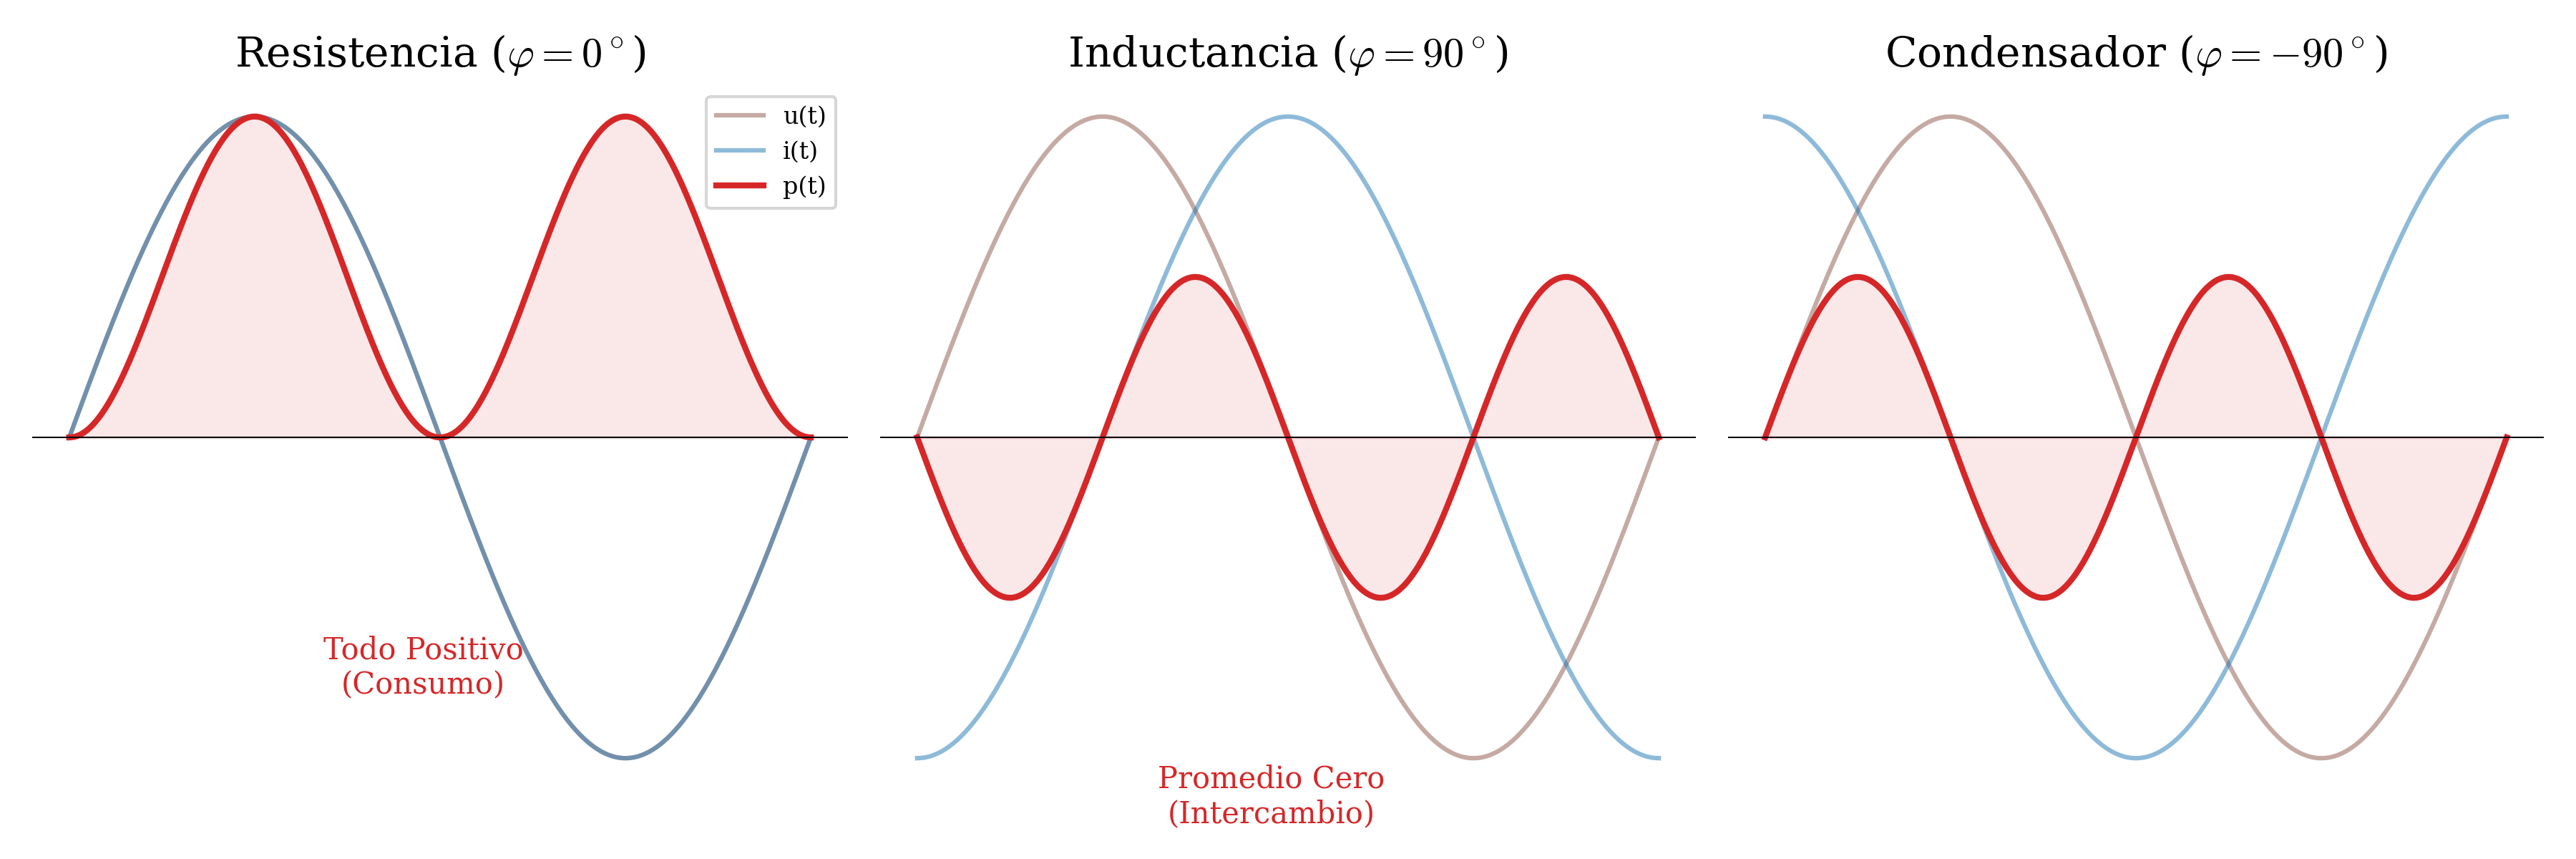
\includegraphics[width=1\linewidth,height=\textheight,keepaspectratio]{media/ondas_potencia.png}

}

\caption{Ondas de potencia instantánea en R, L y C}

\end{figure}%

\begin{longtable}[]{@{}
  >{\raggedright\arraybackslash}p{(\linewidth - 8\tabcolsep) * \real{0.1739}}
  >{\centering\arraybackslash}p{(\linewidth - 8\tabcolsep) * \real{0.2174}}
  >{\centering\arraybackslash}p{(\linewidth - 8\tabcolsep) * \real{0.2174}}
  >{\centering\arraybackslash}p{(\linewidth - 8\tabcolsep) * \real{0.2174}}
  >{\raggedright\arraybackslash}p{(\linewidth - 8\tabcolsep) * \real{0.1739}}@{}}
\caption{Resumen de potencias por
componente.}\label{tbl-potencias-componentes}\tabularnewline
\toprule\noalign{}
\begin{minipage}[b]{\linewidth}\raggedright
Elemento
\end{minipage} & \begin{minipage}[b]{\linewidth}\centering
Desfase (\(\varphi\))
\end{minipage} & \begin{minipage}[b]{\linewidth}\centering
Potencia Activa (\(P\))
\end{minipage} & \begin{minipage}[b]{\linewidth}\centering
Potencia Reactiva (\(Q\))
\end{minipage} & \begin{minipage}[b]{\linewidth}\raggedright
Comportamiento
\end{minipage} \\
\midrule\noalign{}
\endfirsthead
\toprule\noalign{}
\begin{minipage}[b]{\linewidth}\raggedright
Elemento
\end{minipage} & \begin{minipage}[b]{\linewidth}\centering
Desfase (\(\varphi\))
\end{minipage} & \begin{minipage}[b]{\linewidth}\centering
Potencia Activa (\(P\))
\end{minipage} & \begin{minipage}[b]{\linewidth}\centering
Potencia Reactiva (\(Q\))
\end{minipage} & \begin{minipage}[b]{\linewidth}\raggedright
Comportamiento
\end{minipage} \\
\midrule\noalign{}
\endhead
\bottomrule\noalign{}
\endlastfoot
\textbf{Resistencia} & \(0^\circ\) & \textbf{\(U \cdot I\)} & \(0\) &
Consume energía constantemente. \\
\textbf{Bobina} & \(90^\circ\) & \(0\) & \textbf{\(+ U \cdot I\)} &
Absorbe \(Q\) (positiva). No se calienta. \\
\textbf{Condensador} & \(-90^\circ\) & \(0\) & \textbf{\(- U \cdot I\)}
& Cede \(Q\) (negativa). No se calienta. \\
\end{longtable}

\begin{tcolorbox}[enhanced jigsaw, breakable, colback=white, left=2mm, leftrule=.75mm, rightrule=.15mm, toprule=.15mm, colframe=quarto-callout-warning-color-frame, arc=.35mm, bottomrule=.15mm, opacityback=0]

\vspace{-3mm}\textbf{Convenio de Signos para Q}\vspace{3mm}

\begin{itemize}
\tightlist
\item
  \textbf{\(Q > 0\) (Inductiva):} Decimos que el circuito
  \textbf{absorbe} potencia reactiva. El vector \(Q\) apunta hacia
  \textbf{arriba}.
\item
  \textbf{\(Q < 0\) (Capacitiva):} Decimos que el circuito \textbf{cede}
  potencia reactiva (o absorbe negativa). El vector \(Q\) apunta hacia
  \textbf{abajo}.
\end{itemize}

\end{tcolorbox}

\begin{center}\rule{0.5\linewidth}{0.5pt}\end{center}

\section{El Triángulo de Potencias}\label{el-triuxe1ngulo-de-potencias}

Al igual que teníamos un triángulo de impedancias, tenemos un
\textbf{Triángulo de Potencias}. Relaciona las tres magnitudes mediante
Pitágoras.

\begin{figure}

\begin{minipage}{0.60\linewidth}
\textbf{Relaciones Trigonométricas:}

\begin{itemize}
\tightlist
\item
  \textbf{Hipotenusa:} Potencia Aparente (\(\vec{S}\)).
\item
  \textbf{Cateto Horizontal:} Potencia Activa (\(P\)).
\item
  \textbf{Cateto Vertical:} Potencia Reactiva (\(Q\)).
\end{itemize}

Matemáticamente, definimos la \textbf{Potencia Compleja (\(\vec{S}\))}
como:\[
\vec{S} = P + \mathrm{j}Q
\]\end{minipage}%
%
\begin{minipage}{0.40\linewidth}

\begin{figure}[H]

{\centering 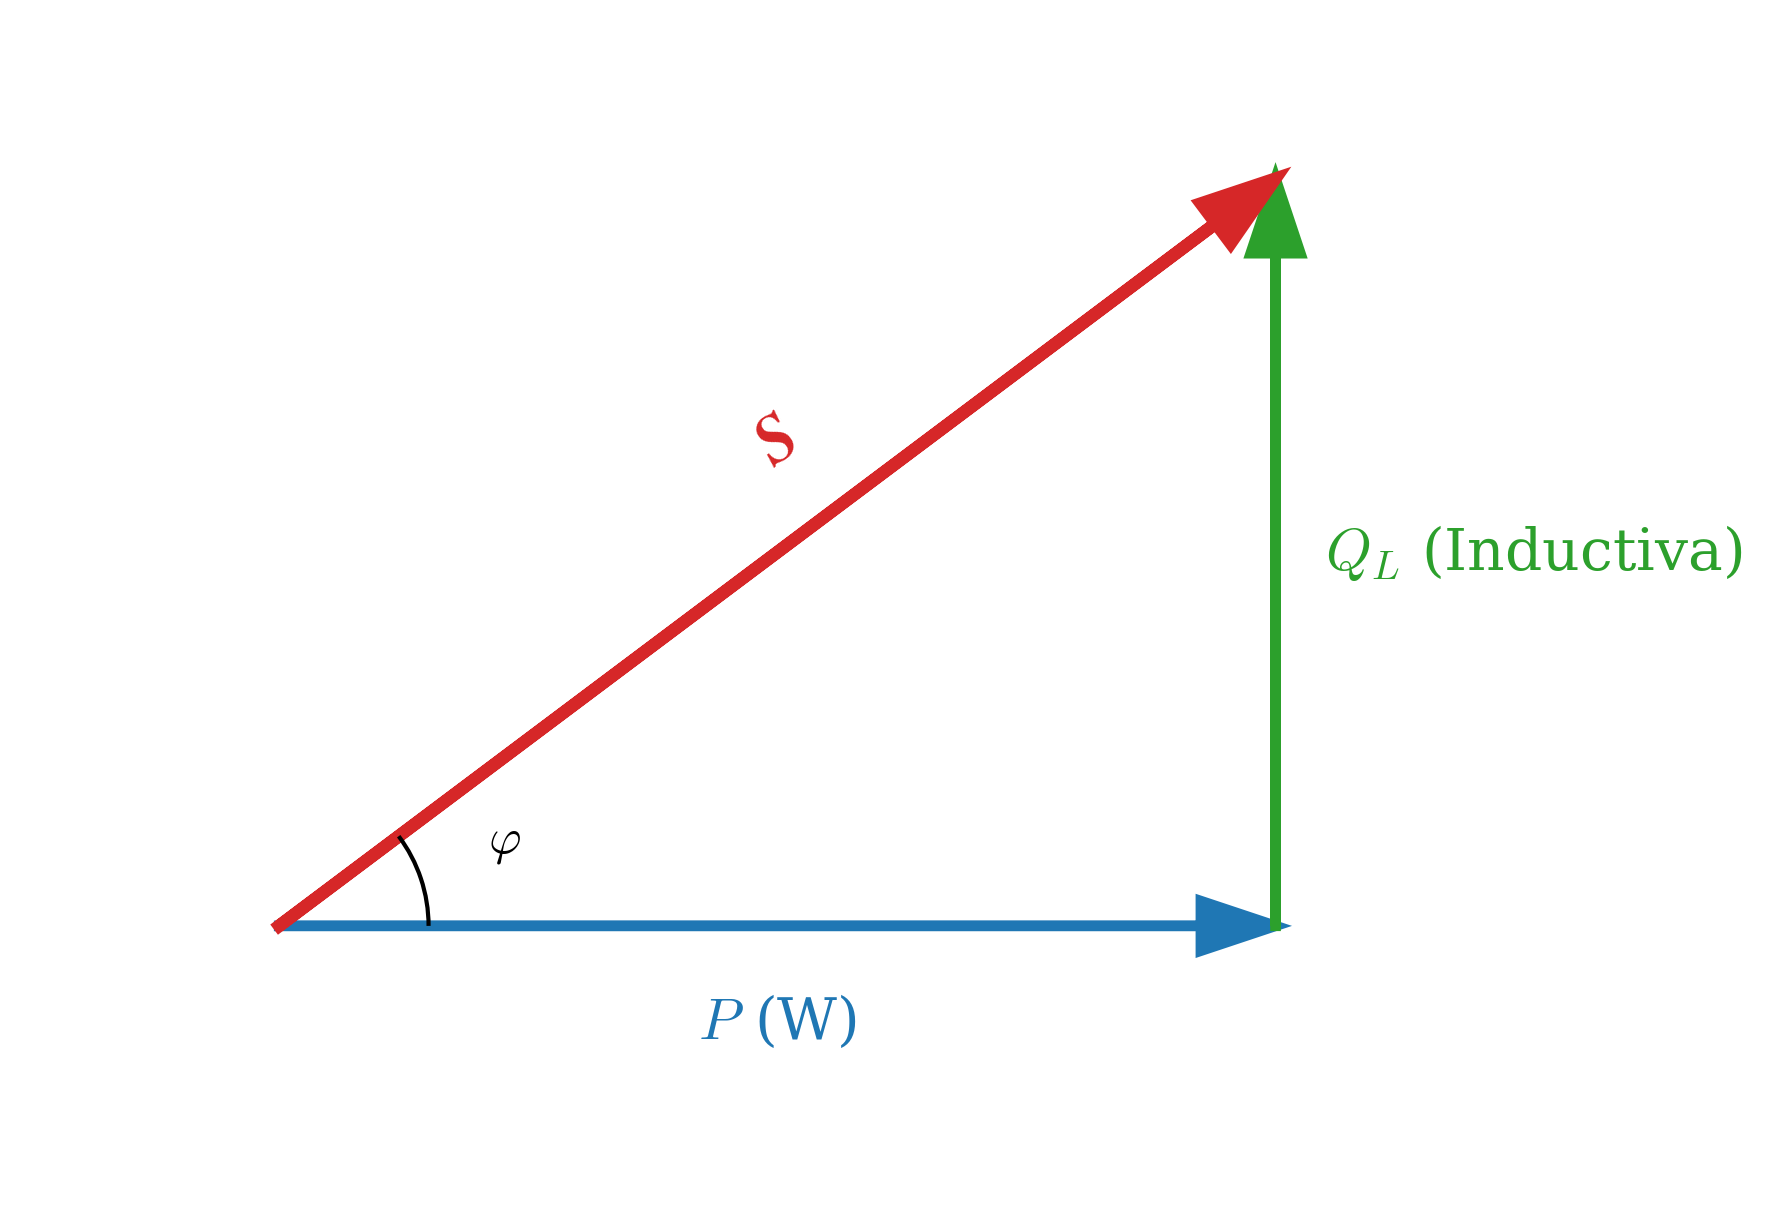
\includegraphics[width=4.16667in,height=\textheight,keepaspectratio]{media/triangulo_potencias_gen.png}

}

\subcaption{Triángulo Inductivo (\(Q>0\))}

\end{figure}%

\end{minipage}%

\end{figure}%

\subsection{\texorpdfstring{El Factor de Potencia
(\(f.d.p.\))}{El Factor de Potencia (f.d.p.)}}\label{el-factor-de-potencia-f.d.p.}

Es un indicador de la \textbf{eficiencia} del sistema. Se define como el
coseno del ángulo \(\varphi\):

\[
f.d.p. = \cos \varphi = \frac{P}{S}
\]

\begin{itemize}
\tightlist
\item
  \textbf{\(\cos \varphi = 1\):} Toda la potencia es útil (\(S=P\)).
  Caso ideal (Resistivo puro).
\item
  \textbf{\(\cos \varphi < 1\):} Parte de la energía se desperdicia
  circulando como reactiva.
\end{itemize}

En el mundo real, la inmensa mayoría de las instalaciones industriales
tienen un \textbf{carácter fuertemente inductivo}. Esto significa que
consumen mucha potencia reactiva positiva (\(Q > 0\)) y tienen un factor
de potencia bajo (\(\cos \varphi < 0,8\)).

\subsection*{¿Por qué el consumo es
Inductivo?}\label{por-quuxe9-el-consumo-es-inductivo}
\addcontentsline{toc}{subsection}{¿Por qué el consumo es Inductivo?}

La razón son las \textbf{Máquinas Eléctricas}. Tanto los
\textbf{motores} (bombas, ventiladores, cintas transportadoras) como los
\textbf{transformadores} funcionan basados en campos magnéticos. Para
crear estos campos magnéticos, necesitan absorber corriente reactiva de
la red para magnetizar sus bobinas.

\subsection*{¿Por qué es necesario
corregirlo?}\label{por-quuxe9-es-necesario-corregirlo}
\addcontentsline{toc}{subsection}{¿Por qué es necesario corregirlo?}

Tener un factor de potencia bajo (\(\cos \varphi\) pequeño) implica
tener un ángulo \(\varphi\) grande, lo que obliga a la empresa eléctrica
a suministrar mucha Potencia Aparente (\(S\)) para conseguir la misma
Potencia Activa (\(P\)).

\[
I = \frac{S}{U} = \frac{P}{U \cdot \cos \varphi}
\]

Si el \(\cos \varphi\) es bajo, la Intensidad Total (\(I\)) se dispara
para mantener la misma potencia útil (\(P\)). Esto provoca:

\vspace{-1em}

\begin{enumerate}
\def\labelenumi{\arabic{enumi}.}
\tightlist
\item
  \textbf{Pérdidas de energía:} Más corriente calienta más los cables
  (efecto Joule).
\item
  \textbf{Sobredimensionamiento:} Se necesitan transformadores y cables
  más gruesos.
\item
  \textbf{Penalizaciones económicas:} Las compañías eléctricas cobran un
  recargo muy alto en la factura si tu factor de potencia es bajo
  (normalmente si es menor de 0,95).
\end{enumerate}

\subsection*{¿Cómo se corrige?
(Compensación)}\label{cuxf3mo-se-corrige-compensaciuxf3n}
\addcontentsline{toc}{subsection}{¿Cómo se corrige? (Compensación)}

La solución consiste en instalar elementos que generen la potencia
reactiva que los motores necesitan, para no tener que pedirla a la red
eléctrica. El elemento ideal es el \textbf{Condensador} (Batería de
Condensadores).

\begin{itemize}
\tightlist
\item
  Los motores \textbf{absorben} \(Q\) (Inductiva, hacia arriba).
\item
  Los condensadores \textbf{ceden} \(Q\) (Capacitiva, hacia abajo).
\end{itemize}

Al conectarlos en paralelo, la \(Q_C\) del condensador cancela gran
parte de la \(Q_L\) del motor.

\begin{figure}

\begin{minipage}{0.50\linewidth}

\begin{figure}[H]

{\centering 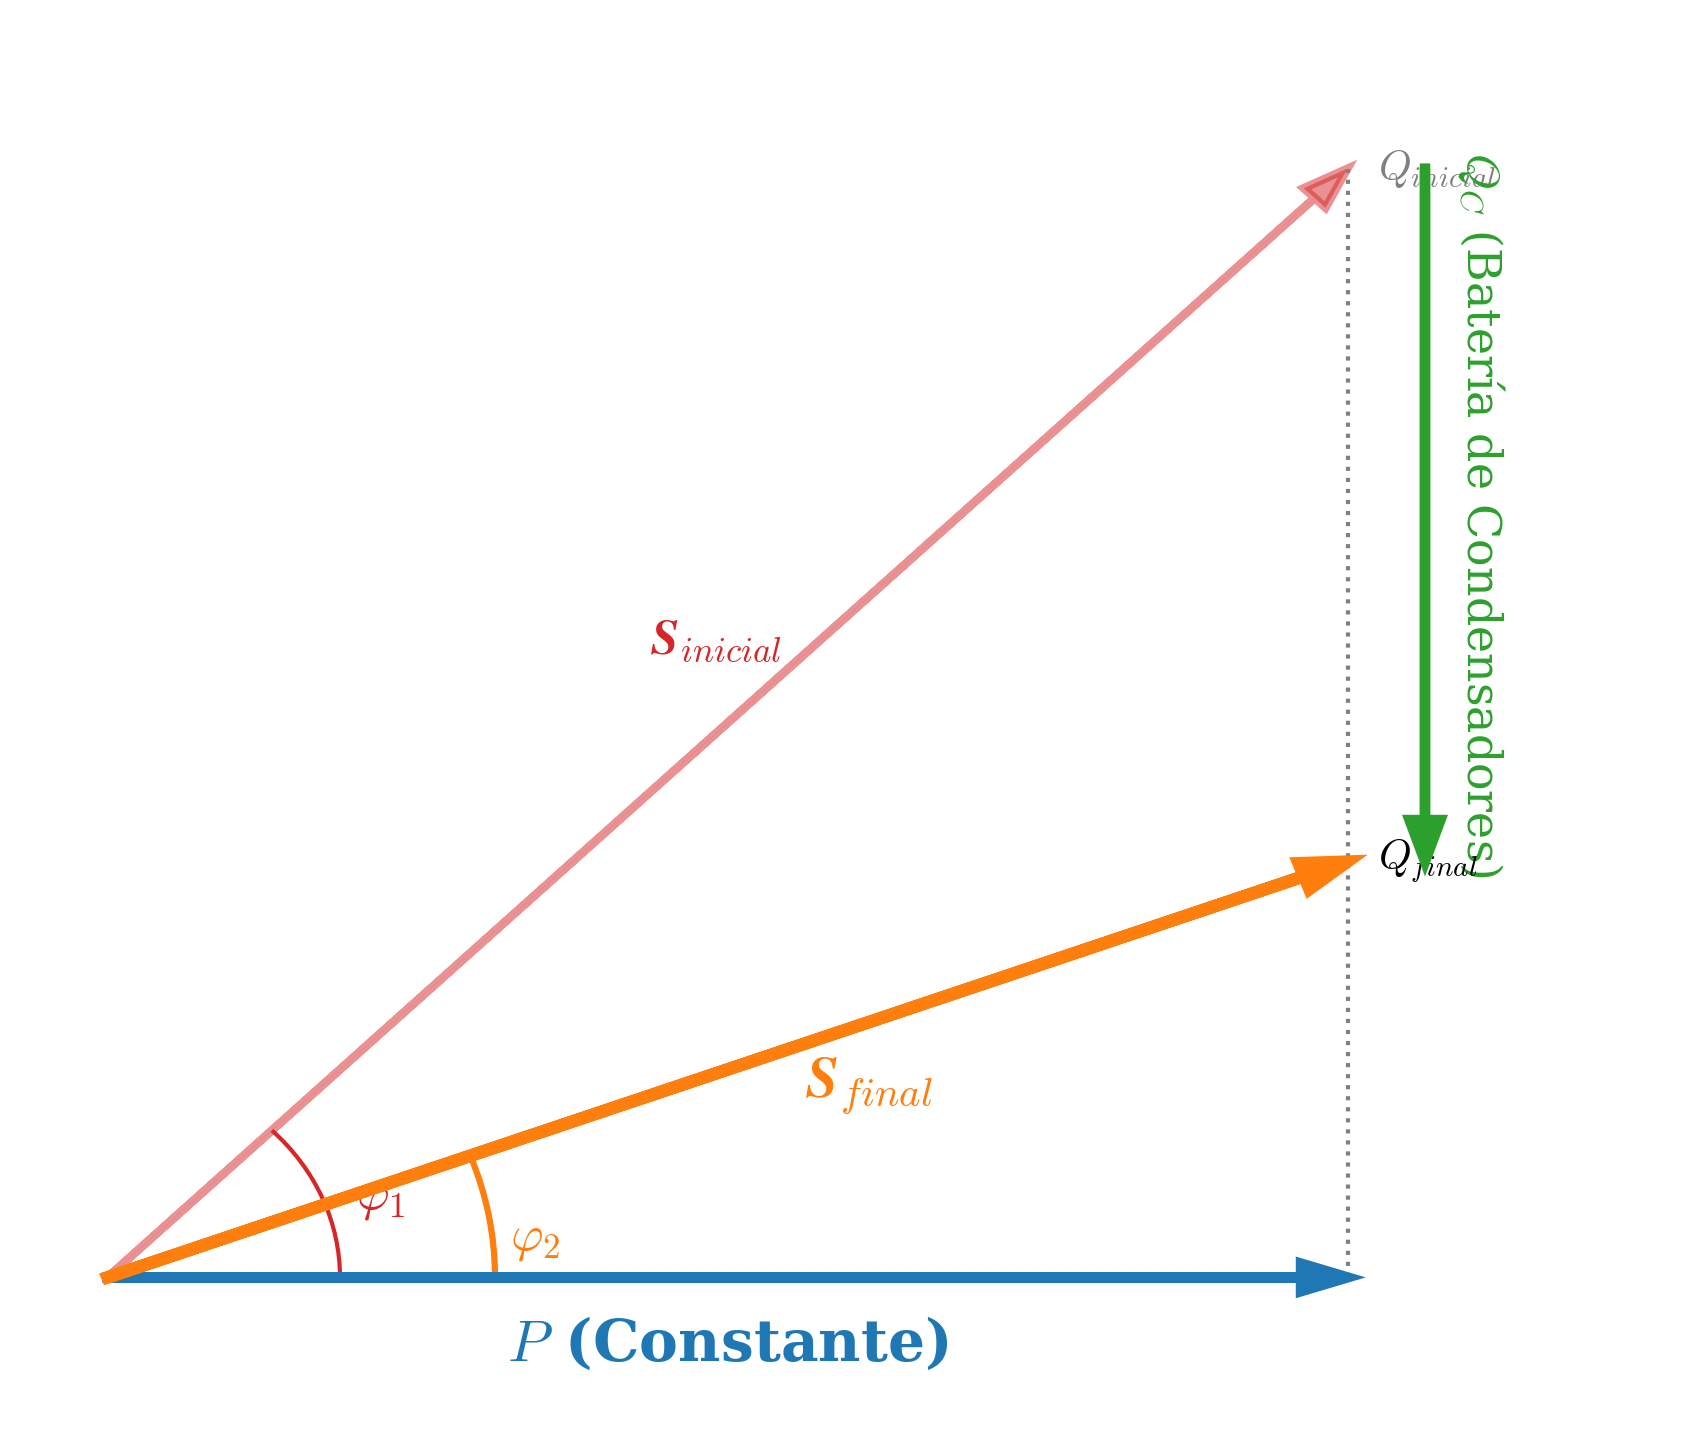
\includegraphics[width=0.9\linewidth,height=\textheight,keepaspectratio]{media/triangulo_compensacion.png}

}

\subcaption{Efecto de la Compensación}

\end{figure}%

\end{minipage}%
%
\begin{minipage}{0.50\linewidth}
\textbf{Análisis del Gráfico:}

\begin{enumerate}
\def\labelenumi{\arabic{enumi}.}
\item
  \textbf{Estado Inicial (Rojo):} Tenemos una carga con mucho consumo de
  reactiva (\(Q_{inicial}\)) y un ángulo \(\varphi_1\) grande. La
  corriente necesaria (\(S_{inicial}\)) es muy alta.
\item
  \textbf{Acción (Verde):} Introducimos una batería de condensadores que
  aporta una \(Q_C\) en sentido contrario (hacia abajo).
\item
  \textbf{Estado Final (Naranja):} La reactiva neta baja a
  \(Q_{final}\).

  \begin{itemize}
  \tightlist
  \item
    La \textbf{Potencia Activa (\(P\)) se mantiene igual} (la máquina
    trabaja igual).
  \item
    La \textbf{Potencia Aparente (\(S_{final}\)) disminuye}.
  \item
    La intensidad total que circula por la línea baja, ahorrando dinero
    y pérdidas.
  \end{itemize}
\end{enumerate}

\end{minipage}%

\end{figure}%

\begin{center}\rule{0.5\linewidth}{0.5pt}\end{center}

\begin{tcolorbox}[enhanced jigsaw, breakable, colback=white, left=2mm, leftrule=.75mm, rightrule=.15mm, toprule=.15mm, colframe=quarto-callout-important-color-frame, arc=.35mm, bottomrule=.15mm, opacityback=0]

\vspace{-3mm}\textbf{💡 Ejemplo Resuelto: Motor Monofásico}\vspace{3mm}

Un motor eléctrico (carga inductiva) se conecta a una red de
\(230\ \text{V}\). Consume una intensidad de \(5\ \text{A}\) con un
factor de potencia de \(\mathbf{0,8}\) (inductivo). Calcula \(P, Q, S\)
y dibuja el triángulo.

\textbf{Solución:}

\begin{enumerate}
\def\labelenumi{\arabic{enumi}.}
\item
  \textbf{Potencia Aparente (\(S\)):} Es lo primero que podemos calcular
  con \(U\) e \(I\).
  \[S = U \cdot I = 230 \cdot 5 = \mathbf{1150\ \text{VA}}\]
\item
  \textbf{Ángulo (\(\varphi\)):}
  \[\cos \varphi = 0,8 \Rightarrow \varphi = \arccos(0,8) = 36,87^\circ\]
  Como es inductivo, \(\varphi > 0\).
\item
  \textbf{Potencia Activa (\(P\)):}
  \[P = S \cdot \cos \varphi = 1150 \cdot 0,8 = \mathbf{920\ \text{W}}\]
\item
  \textbf{Potencia Reactiva (\(Q\)):} Calculamos el seno:
  \(\sen(36,87^\circ) = 0,6\).
  \[Q = S \cdot \sen \varphi = 1150 \cdot 0,6 = \mathbf{690\ \text{var}}\]
\end{enumerate}

\begin{figure}[H]

\begin{minipage}{0.50\linewidth}
\textbf{Triángulo de Potencias:} Como es inductivo, la \(Q\) se dibuja
hacia arriba.
\[\vec{S} = 920 + \mathrm{j}690\ \text{VA}\]\end{minipage}%
%
\begin{minipage}{0.50\linewidth}

\begin{figure}[H]

{\centering 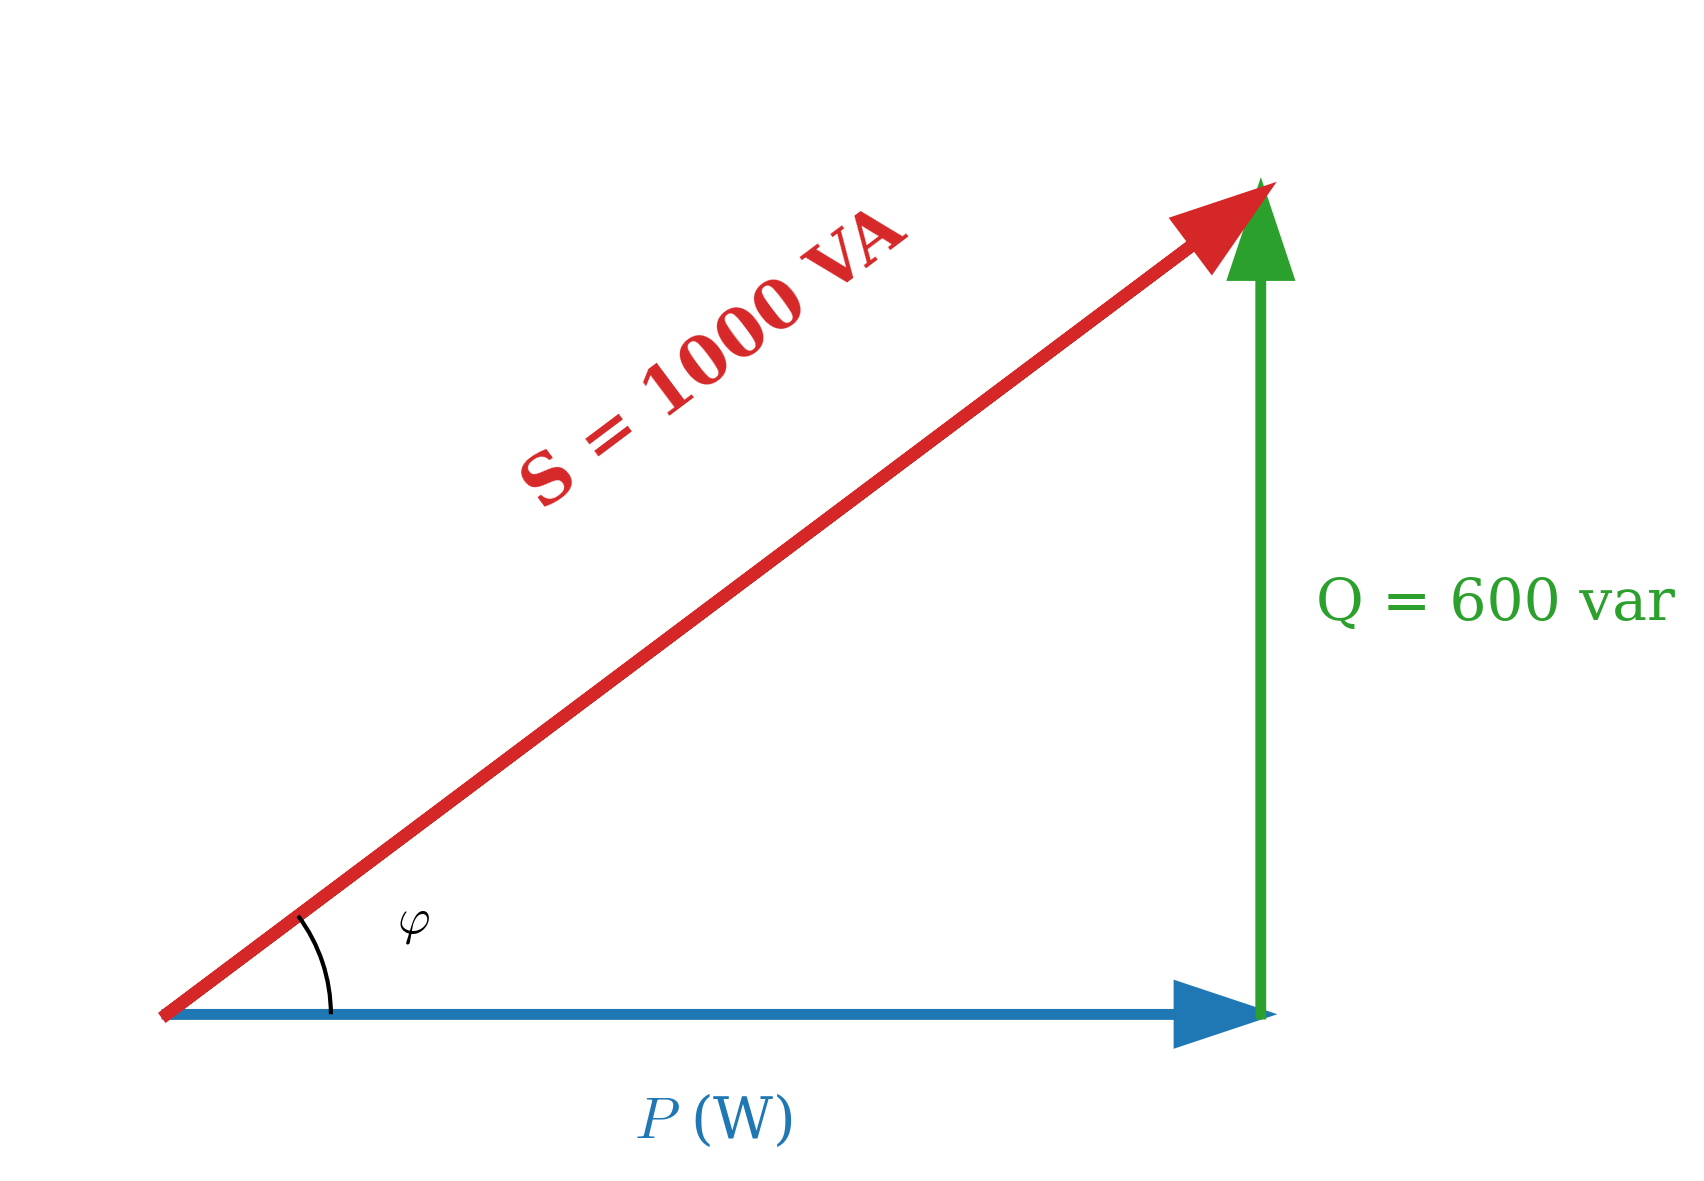
\includegraphics[width=0.8\linewidth,height=\textheight,keepaspectratio]{media/triangulo_potencias_ejemplo.png}

}

\subcaption{Triángulo del Motor}

\end{figure}%

\end{minipage}%

\end{figure}%

\end{tcolorbox}

\begin{center}\rule{0.5\linewidth}{0.5pt}\end{center}

\section{Ejercicios Propuestos}\label{ejercicios-propuestos-1}

\begin{tcolorbox}[enhanced jigsaw, breakable, colback=white, left=2mm, leftrule=.75mm, rightrule=.15mm, toprule=.15mm, colframe=quarto-callout-important-color-frame, arc=.35mm, bottomrule=.15mm, opacityback=0]

\vspace{-3mm}\textbf{📝 Practica tú mismo}\vspace{3mm}

\textbf{1.} Una estufa de resistencia pura \(R=50\ \Omega\) se conecta a
\(230\ \text{V}\).\\
\strut ~~~~~~ \textbf{a)} Calcula su potencia activa, reactiva y
aparente.\\
\strut ~~~~~~ \textbf{b)} ¿Cuánto vale su factor de potencia?

\emph{Soluciones:} \(P=1058\ \text{W}\); \(Q=0\); \(S=1058\ \text{VA}\);
\(\cos\varphi=1\).

\begin{center}\rule{0.5\linewidth}{0.5pt}\end{center}

\textbf{2.} Un condensador de \(C=100\ \mu\text{F}\) se conecta a
\(230\ \text{V}\) / \(50\ \text{Hz}\).\\
\strut ~~~~~~ \textbf{a)} Calcula la reactancia \(X_C\) y la potencia
reactiva \(Q\).\\
\strut ~~~~~~ \textbf{b)} ¿Absorbe o cede potencia reactiva?

\emph{Soluciones:} \(X_C=31,83\ \Omega\); \(Q = -1661\ \text{var}\);
Cede reactiva (Capacitivo).

\begin{center}\rule{0.5\linewidth}{0.5pt}\end{center}

\textbf{3.} Una instalación consume una potencia activa
\(P=3000\ \text{W}\) y una reactiva inductiva \(Q=4000\ \text{var}\).\\
\strut ~~~~~~ \textbf{a)} Calcula la potencia aparente total.\\
\strut ~~~~~~ \textbf{b)} Halla el factor de potencia.\\
\strut ~~~~~~ \textbf{c)} Si la tensión es \(230\ \text{V}\), ¿qué
corriente circula por el cable general?

\emph{Soluciones:} \(S=5000\ \text{VA}\); \(\cos\varphi=0,6\);
\(I=21,74\ \text{A}\).

\begin{center}\rule{0.5\linewidth}{0.5pt}\end{center}

\textbf{4.}En el circuito de la figura, calcular:\\
\strut ~~~ \textbf{a)} La intensidad que circula por cada rama.\\
\strut ~~~ \textbf{b)} La impedancia equivalente vista desde el
generador.\\
\strut ~~~ \textbf{c)} Las potencias activa y reactiva totales.

\textbf{Datos:} \(X_{C2}=10\ \Omega\); \(X_{C1} = X_L = R = 5\ \Omega\);
\(E = 50\ \text{V}\).

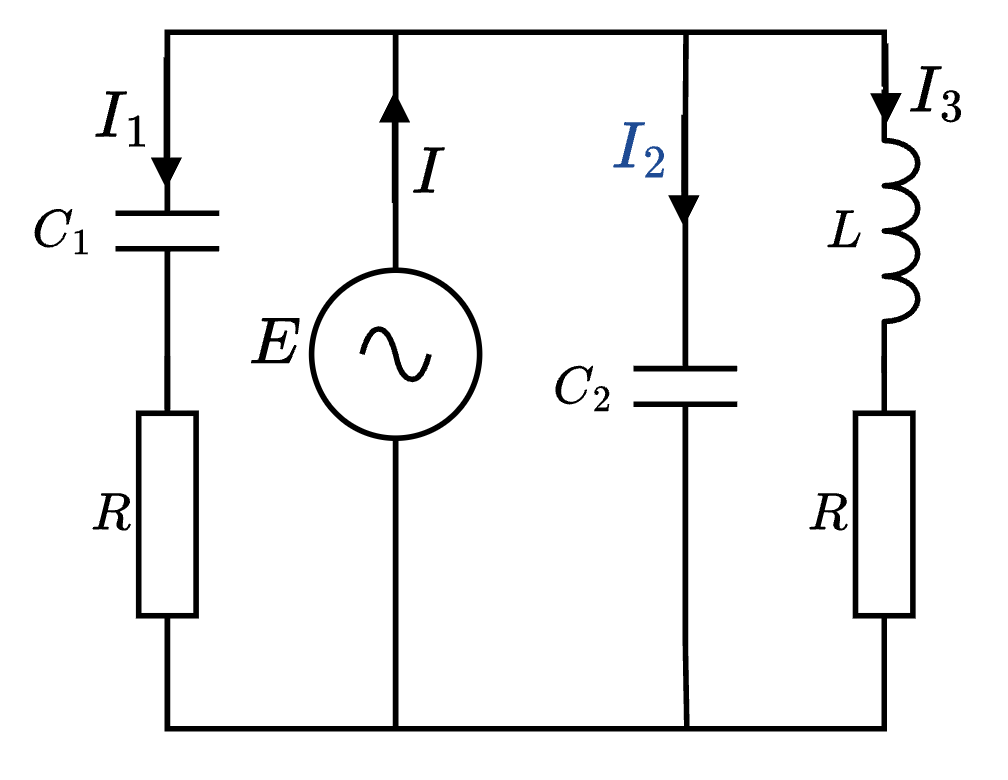
\includegraphics[width=4.16667in,height=\textheight,keepaspectratio]{media/ejercicio_potencia4.png}

\textbf{Soluciones:} \textbf{a)}
\(\vec{I}_{\text{Rama1}} = 5 \sqrt{2} \phase 45^\circ\ \text{A}\);
\(\quad \vec{I}_{\text{Rama2}} = 5 \phase 90^\circ\ \text{A}\);\(\vec{I}_{\text{Rama3}} = 5 \sqrt{2} \phase -45^\circ\ \text{A}\);
\textbf{b)} \(\vec{Z}_{eq} = 4 + 2\mathrm{j}\ \Omega\)
(\(2 \sqrt{5} \phase 26,56^\circ\ \Omega\)). \textbf{c)}
\(P_T = 500\ \text{W}\); \(\quad Q_T = 250\ \text{var}\) (Inductiva).

\begin{center}\rule{0.5\linewidth}{0.5pt}\end{center}

\textbf{5.} En el circuito de la figura se muestra un circuito de
corriente alterna en el que las indicaciones de los aparatos de medida,
supuestos ideales, son las siguientes:

\begin{itemize}
\tightlist
\item
  Voltímetro, \(100\ \text{V}\) (valor eficaz).
\item
  Amperímetro, \(20\ \text{A}\) (valor eficaz).
\item
  Vatímetro, \(1200\ \text{W}\).
\end{itemize}

Hallar \(\vec{Z}\), \(R\), \(X\) y \(\vec{U}_s\), tomando \(\vec{I}\)
como origen de fases.

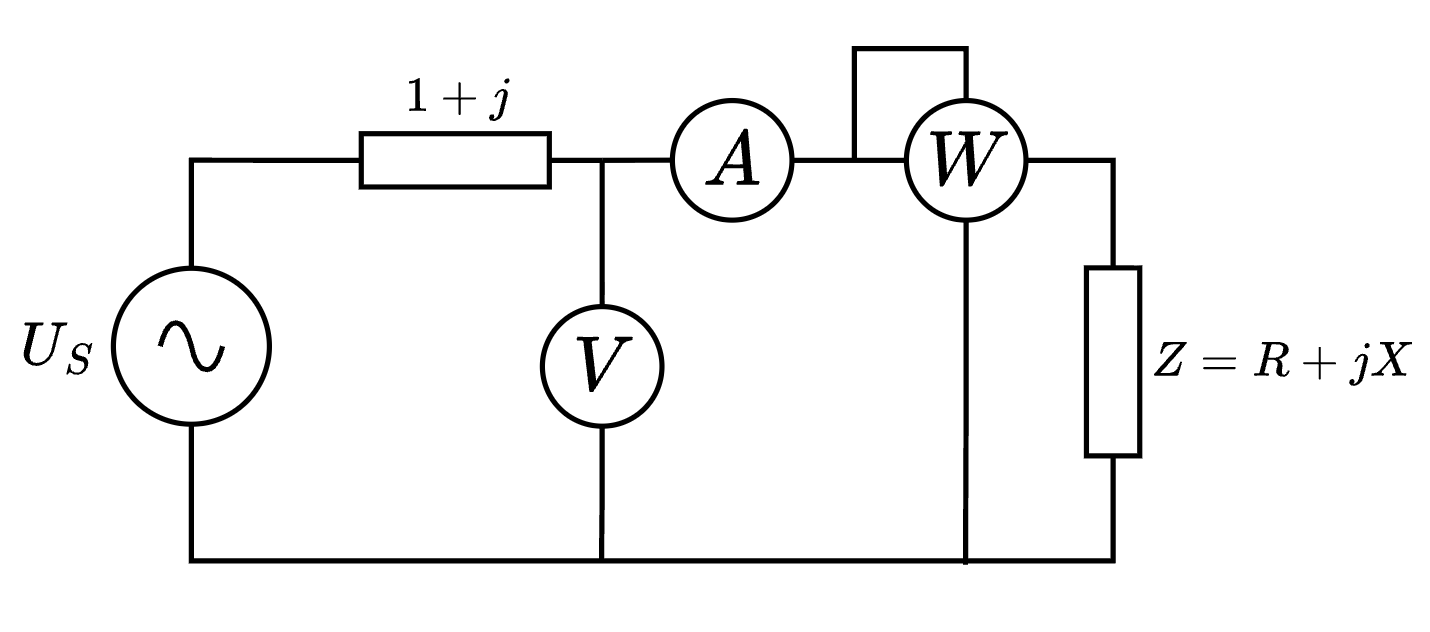
\includegraphics[width=0.6\linewidth,height=\textheight,keepaspectratio]{media/ejercicio_potencia5.png}

\textbf{Soluciones:} \textbf{Impedancia:}
\(\vec{Z} = 3 + \mathrm{j}4\ \Omega\)
(\(5 \phase 53,13^\circ\ \Omega\)). \textbf{Componentes:}
\(R = 3\ \Omega\); \(\quad X = 4\ \Omega\). \textbf{Tensión fuente:}
\(\vec{U}_s = 80 + 100\mathrm{j}\ \text{V}\)
(\(128 \phase 51,31^\circ\ \text{V}\)).

\begin{center}\rule{0.5\linewidth}{0.5pt}\end{center}

\textbf{6.} El circuito de la figura se alimenta con una fuente de
tensión de valor eficaz \(220\text{V}/50\text{Hz}\). Se pide:\\
\strut ~~~ \textbf{a)} Calcular el valor de la lectura del amperímetro
A.\\
\strut ~~~ \textbf{b)} Determinar la lectura del voltímetro V.\\
\strut ~~~ \textbf{c)} Calcular las potencias totales consumidas en el
circuito y representar el triángulo de potencias.

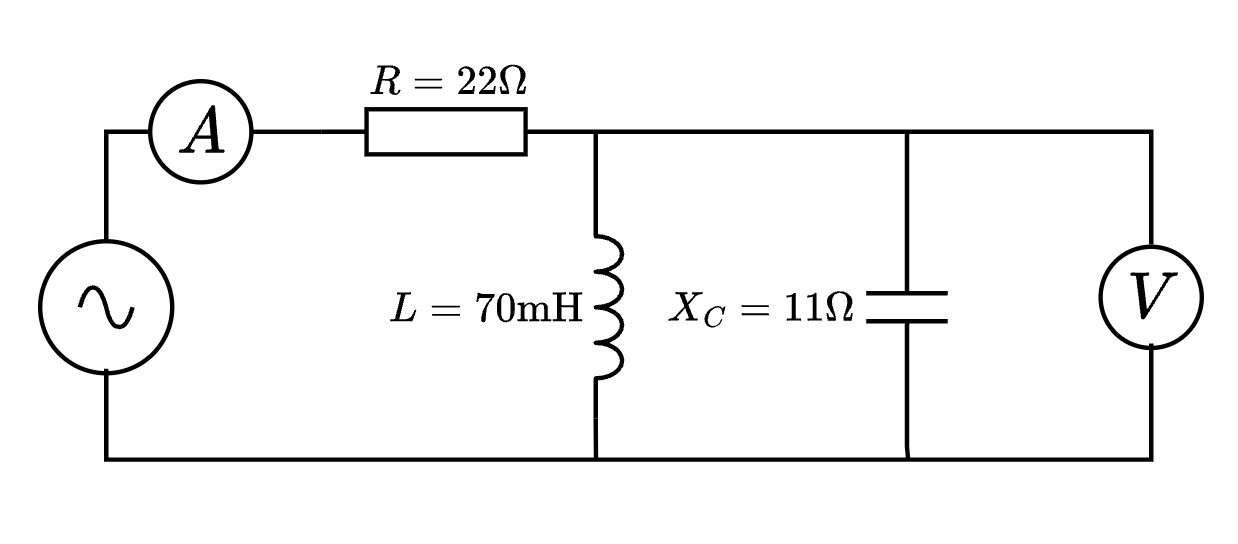
\includegraphics[width=0.6\linewidth,height=\textheight,keepaspectratio]{media/ejercicio_potencia6.png}

\textbf{Soluciones:} \textbf{a)} Lectura A \(= 5 \sqrt{2}\ \text{A}\).
\textbf{b)} Lectura V \(= 155,56\ \text{V}\). \textbf{c)}
\(P = 1100\ \text{W}\); \(\quad Q = -1100\ \text{var}\);
\(\quad S = 1555,63\ \text{VA}\).

\begin{center}\rule{0.5\linewidth}{0.5pt}\end{center}

\textbf{7.} En el circuito de la figura se sabe que los elementos R-L
constituyen una carga que absorbe \(2000\ \text{W}\) con el factor de
potencia 0,5 si se cortocircuita el condensador C. Si la tensión de la
fuente es de \(220\ \text{V}/50\text{Hz}\), calcula el valor que debe
tener el condensador para que el factor de potencia del conjunto R-L-C
sea unitario.

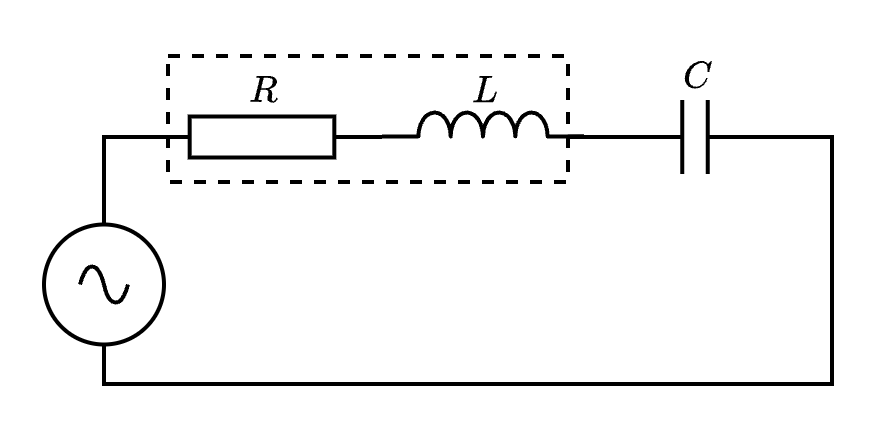
\includegraphics[width=4.16667in,height=\textheight,keepaspectratio]{media/ejercicio_potencia7.png}

\textbf{Solución: \(C = 36,75\ \mu\text{F}\).}

\begin{center}\rule{0.5\linewidth}{0.5pt}\end{center}

\textbf{8.} Se conecta a una línea de \(220\ \text{V}\) un receptor
monofásico inductivo (motor eléctrico) que consume una potencia activa
de \(5\ \text{kW}\) con un factor de potencia de \(0,7\). Se pide:

~~~ \textbf{a)} Calcular las potencias reactiva y aparente.\\
\strut ~~~ \textbf{b)} Calcular la capacidad equivalente del condensador
que se ha de conectar si se desea mejorar el factor de potencia a
\(0,95\).\\
\strut ~~~ \textbf{c)} Calcular la reducción de corriente por la línea
al conectar el condensador.\\
\strut ~~~ \textbf{d)} ¿Ha cambiado la potencia activa al mejorar el
factor de potencia? Justifica la respuesta.

\textbf{Soluciones:} \textbf{a)} \(S = 7142,8\ \text{VA}\);
\(\quad Q = 5101\ \text{var}\). \textbf{b)}
\(Q_C = 3457,5\ \text{var} \Rightarrow C = 227,4\ \mu\text{F}\).
\textbf{c)} La corriente baja de \(32,47\ \text{A}\) a
\(23,92\ \text{A}\). Reducción: \(\Delta I = 8,55\ \text{A}\).
\textbf{d)} No.~La potencia activa (\(P\)) depende del trabajo que
realiza el motor, y eso no cambia al añadir condensadores en paralelo.

\begin{center}\rule{0.5\linewidth}{0.5pt}\end{center}

\textbf{9.} Una carga de corriente alterna monofásica de
\(50\ \text{Hz}\) es alimentada a una tensión de \(220\ \text{V}\)
(valor eficaz). Sabiendo que la potencia aparente absorbida por dicha
carga es de \(20\ \text{kVA}\), con \(\cos \varphi = 0,8\) inductivo, se
pide:

~~~ \textbf{a)} Las potencias activa y reactiva consumidas por la
carga.\\
\strut ~~~ \textbf{b)} La impedancia compleja de la carga.\\
\strut ~~~ \textbf{c)} El condensador que conectado en paralelo con la
carga hace que el factor de potencia de la instalación sea \(0,95\)
inductivo.

\textbf{Soluciones:} \textbf{a)} \(P = 16\ \text{kW}\);
\(\quad Q = 12\ \text{kvar}\). \textbf{b)}
\(\vec{Z} = 1,936 + \mathrm{j}1,452\ \Omega\)
(\(2,42 \angle 36,87^\circ\ \Omega\)). \textbf{c)}
\(Q_C = 6740,8\ \text{var} \Rightarrow C = 443,3\ \mu\text{F}\).

\end{tcolorbox}

\cleardoublepage
\phantomsection
\addcontentsline{toc}{part}{Appendices}
\appendix

\chapter{Números Complejos en CA}\label{sec-anexo-complejos}

El análisis de circuitos de corriente alterna se simplifica enormemente
utilizando números complejos. A continuación, se presenta un resumen de
las propiedades y operaciones fundamentales para su consulta rápida.

\section{Definición y Forma
Binómica}\label{definiciuxf3n-y-forma-binuxf3mica}

Un número complejo es una expresión de la forma:
\[\vec{Z} = a + \mathrm{j} \cdot b\]

Donde:

\begin{itemize}
\tightlist
\item
  \(a\) es la \textbf{parte real} (\(a \in \mathbb{R}\)).
\item
  \(b\) es la \textbf{parte imaginaria} (\(b \in \mathbb{R}\)).
\item
  \(\mathrm{j}\) es la unidad imaginaria, definida como
  \(\mathrm{j} = \sqrt{-1}\).
\end{itemize}

\begin{tcolorbox}[enhanced jigsaw, breakable, colback=white, left=2mm, leftrule=.75mm, rightrule=.15mm, toprule=.15mm, colframe=quarto-callout-note-color-frame, arc=.35mm, bottomrule=.15mm, opacityback=0]

\vspace{-3mm}\textbf{Definiciones Básicas}\vspace{3mm}

\begin{enumerate}
\def\labelenumi{\arabic{enumi}.}
\tightlist
\item
  \textbf{Igualdad:} Dos números complejos \(\vec{Z} = a + \mathrm{j}b\)
  y \(\vec{W} = c + \mathrm{j}d\) son iguales si sus partes reales e
  imaginarias coinciden (\(a=c\) y \(b=d\)).
\item
  \textbf{Conjugado:} El conjugado de un número \(\vec{Z}\), denotado
  como \(\vec{Z}^*\), es aquel que tiene la misma parte real y la parte
  imaginaria opuesta (\(\vec{Z}^* = a - \mathrm{j} \cdot b\)).
\item
  \textbf{Producto por el conjugado:} Al multiplicar un número complejo
  por su conjugado, se obtiene siempre un \textbf{número real}.
  \[\vec{Z} \cdot \vec{Z}^* = a^2 + b^2\] \emph{Esta propiedad es
  fundamental para eliminar la ``j'' de los denominadores al dividir.}
\end{enumerate}

\end{tcolorbox}

\section{Operaciones en Forma
Binómica}\label{operaciones-en-forma-binuxf3mica}

Dados dos números complejos \(\vec{Z} = a + \mathrm{j}b\) y
\(\vec{W} = c + \mathrm{j}d\):

\begin{itemize}
\item
  \textbf{Suma y Resta:} Se suman (o restan) las partes reales entre sí
  y las imaginarias entre sí.
  \[\vec{Z} \pm \vec{W} = (a \pm c) + \mathrm{j}(b \pm d)\]
\item
  \textbf{Producto:} Se aplica la propiedad distributiva, recordando que
  \(\mathrm{j}^2 = -1\).
  \[\vec{Z} \cdot \vec{W} = (ac - bd) + \mathrm{j}(ad + bc)\]
\item
  \textbf{División:} Se multiplica numerador y denominador por el
  conjugado del denominador para eliminar la parte imaginaria de abajo.
  \[\frac{\vec{Z}}{\vec{W}} = \frac{ac+bd}{c^2+d^2} + \mathrm{j} \frac{bc-ad}{c^2+d^2}\]
\end{itemize}

\section{Representación Gráfica y Forma
Polar}\label{representaciuxf3n-gruxe1fica-y-forma-polar}

Los números complejos se representan en el plano complejo (diagrama de
Argand), donde el eje horizontal es la parte real y el vertical la
imaginaria.

\begin{figure}[H]

\centering{

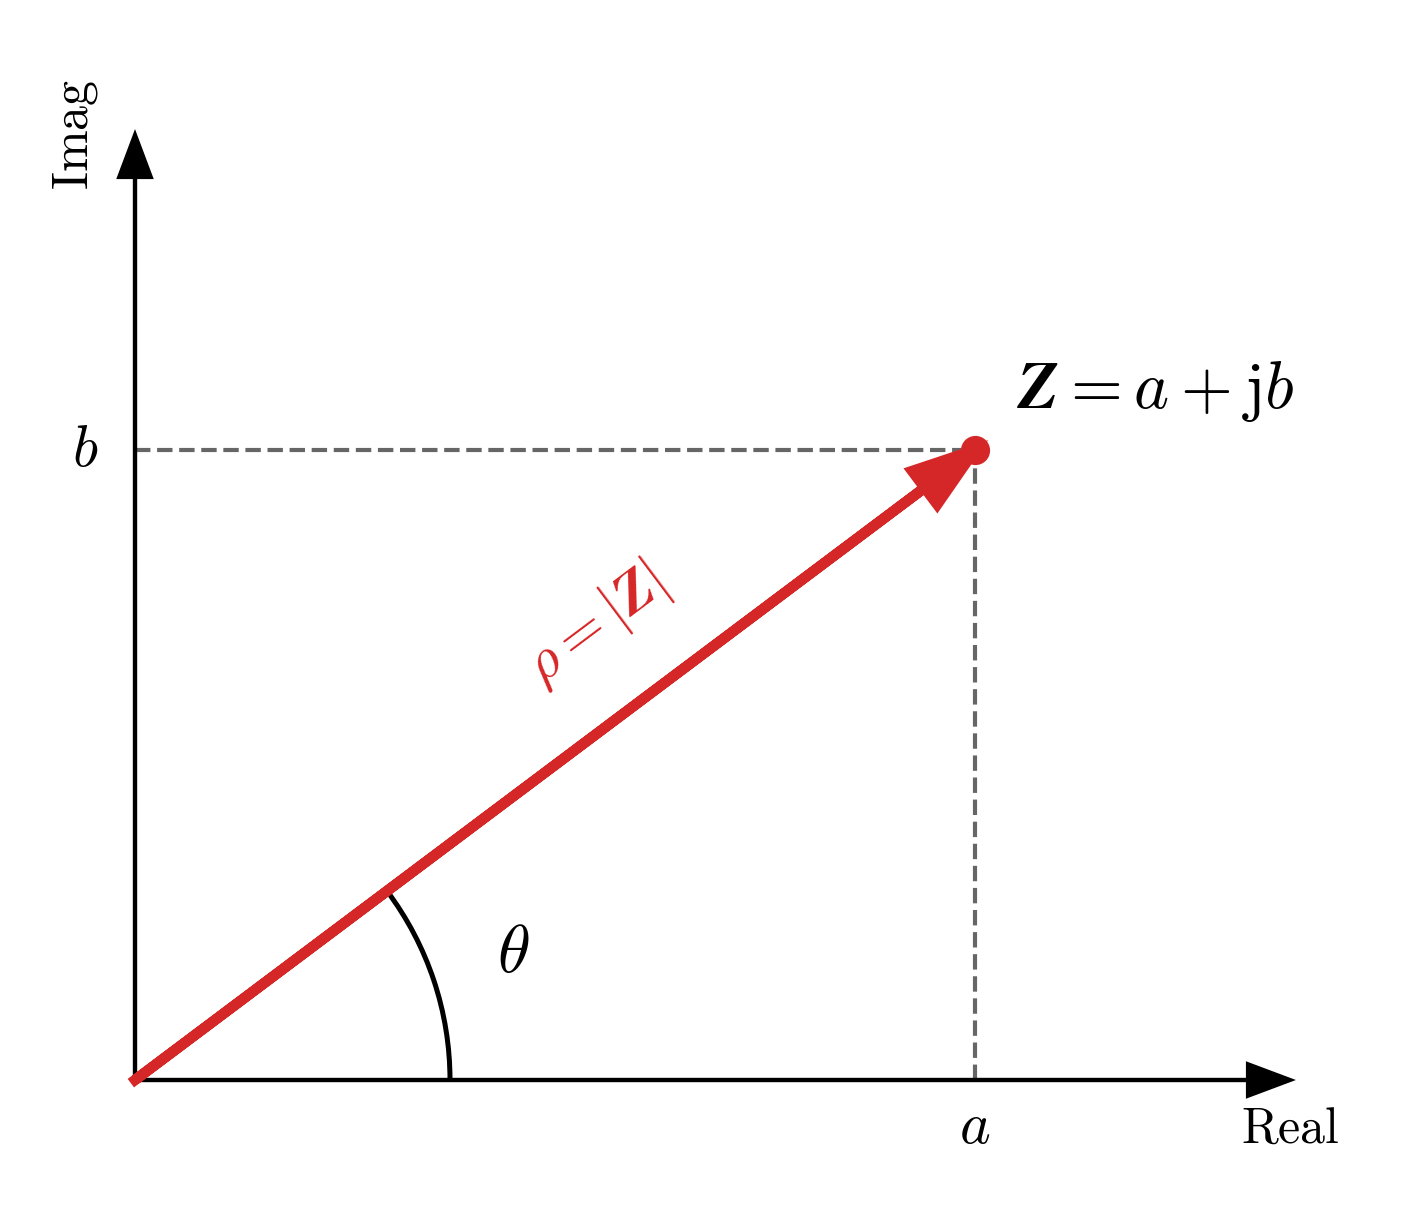
\includegraphics[width=0.6\linewidth,height=\textheight,keepaspectratio]{media/plano_complejo.png}

}

\caption{\label{fig-plano-complejo}Representación vectorial de un número
complejo}

\end{figure}%

A partir de la gráfica, definimos la \textbf{forma polar} mediante el
\textbf{módulo} (\(|\vec{Z}|\) o \(\rho\)) y el \textbf{argumento}
(\(\theta\)):

\[\vec{Z} = \rho \angle \theta\]

\subsection{Conversión entre formas}\label{conversiuxf3n-entre-formas}

\begin{figure}

\begin{minipage}{0.50\linewidth}
\textbf{De Binómica a Polar:} \[
\begin{aligned}
\rho &= |\vec{Z}| = \sqrt{a^2 + b^2} \\
\theta &= \arctan\left(\frac{b}{a}\right)
\end{aligned}
\]\end{minipage}%
%
\begin{minipage}{0.50\linewidth}
\textbf{De Polar a Binómica:} \[
\begin{aligned}
a &= \rho \cdot \cos \theta \\
b &= \rho \cdot \sen \theta
\end{aligned}
\]\end{minipage}%

\end{figure}%

\section{Operaciones en Forma Polar}\label{operaciones-en-forma-polar}

La forma polar es mucho más eficiente para realizar multiplicaciones y
divisiones. Dados dos números \(\vec{Z} = \rho \angle \theta\) y
\(\vec{W} = \sigma \angle \delta\):

\begin{itemize}
\item
  \textbf{Producto:} Se multiplican los módulos y se \textbf{suman} los
  argumentos.
  \[\vec{Z} \cdot \vec{W} = (\rho \cdot \sigma) \angle (\theta + \delta)\]
\item
  \textbf{División:} Se dividen los módulos y se \textbf{restan} los
  argumentos.
  \[\frac{\vec{Z}}{\vec{W}} = \left( \frac{\rho}{\sigma} \right) \angle (\theta - \delta)\]
\item
  \textbf{Conjugado:} El conjugado en polar mantiene el módulo y cambia
  el signo del ángulo. \[\vec{Z}^* = \rho \angle (-\theta)\]
\end{itemize}

\begin{center}\rule{0.5\linewidth}{0.5pt}\end{center}

\begin{tcolorbox}[enhanced jigsaw, breakable, colback=white, left=2mm, leftrule=.75mm, rightrule=.15mm, toprule=.15mm, colframe=quarto-callout-important-color-frame, arc=.35mm, bottomrule=.15mm, opacityback=0]

\vspace{-3mm}\textbf{💡 Regla de Oro para el Cálculo en CA}\vspace{3mm}

Para optimizar el trabajo y evitar errores al resolver circuitos, sigue
siempre este criterio:

\begin{enumerate}
\def\labelenumi{\arabic{enumi}.}
\tightlist
\item
  \textbf{Para Sumas y Restas:} Utiliza obligatoriamente la
  \textbf{Forma Binómica} (\(\vec{Z} = a + \mathrm{j}b\)).

  \begin{itemize}
  \tightlist
  \item
    \emph{Intentar sumar en polar es un error muy común y
    matemáticamente incorrecto sin pasar antes a binómica.}
  \end{itemize}
\item
  \textbf{Para Multiplicaciones y Divisiones:} Utiliza preferiblemente
  la \textbf{Forma Polar} (\(\vec{Z} = \rho \angle \theta\)).

  \begin{itemize}
  \tightlist
  \item
    \emph{Es mucho más rápido y menos propenso a errores multiplicar
    módulos y sumar ángulos que hacer la distributiva con las ``j''.}
  \end{itemize}
\end{enumerate}

\end{tcolorbox}

\section{Guía Rápida de Uso de la
Calculadora}\label{guuxeda-ruxe1pida-de-uso-de-la-calculadora}

Aunque cada modelo es diferente, la mayoría de calculadoras científicas
estándar siguen una lógica similar para trabajar con números complejos.

\subsection{Configuración Inicial}\label{configuraciuxf3n-inicial}

Antes de empezar a operar, asegúrate de dos cosas fundamentales:

\begin{enumerate}
\def\labelenumi{\arabic{enumi}.}
\tightlist
\item
  \textbf{Activa el Modo Complejo:} Busca la tecla \texttt{MODE} o
  \texttt{SETUP} y selecciona la opción \textbf{CMPLX} (o
  \emph{Complex}).

  \begin{itemize}
  \tightlist
  \item
    \emph{Sabrás que está activo si ves un indicador ``CPLX'' o
    ``CMPLX'' en la pantalla.}
  \end{itemize}
\item
  \textbf{Verifica los Grados:} Asegúrate de que la calculadora está en
  \textbf{Degrees (D)} (Grados sexagesimales) y no en Radianes (R) o
  Gradianes (G).

  \begin{itemize}
  \tightlist
  \item
    \emph{Si ves una ``R'' en la pantalla, tus resultados angulares
    saldrán mal.}
  \end{itemize}
\end{enumerate}

\subsection{Cómo escribir los
números}\label{cuxf3mo-escribir-los-nuxfameros}

Ten en cuenta que las calculadoras usan la notación matemática estándar
(\(i\)) en lugar de la notación eléctrica (\(\mathrm{j}\)).

\begin{itemize}
\tightlist
\item
  \textbf{La unidad imaginaria (\(i\)):} Suele estar en la tecla
  \texttt{ENG}. En la mayoría de modelos no hace falta pulsar
  \emph{Shift} antes.

  \begin{itemize}
  \tightlist
  \item
    \emph{Ejemplo para escribir \(3 + \mathrm{j}4\):} Teclea \texttt{3}
    \texttt{+} \texttt{4} \texttt{i}.
  \end{itemize}
\item
  \textbf{El símbolo de ángulo (\(\angle\)):} Para introducir formas
  polares, busca el símbolo \(\angle\) (suele estar sobre la tecla
  \texttt{(-)} o \texttt{v} y requiere pulsar \texttt{SHIFT}).

  \begin{itemize}
  \tightlist
  \item
    \emph{Ejemplo para escribir \(10 \angle 30^\circ\):} Teclea
    \texttt{10} \texttt{SHIFT} \texttt{\textbackslash{}angle}
    \texttt{30}.
  \end{itemize}
\end{itemize}

\subsection{Conversión entre formas (Paso a
paso)}\label{conversiuxf3n-entre-formas-paso-a-paso}

El error más común es no saber cómo pasar un resultado de binómica a
polar o viceversa.

\begin{tcolorbox}[enhanced jigsaw, breakable, colback=white, left=2mm, leftrule=.75mm, rightrule=.15mm, toprule=.15mm, colframe=quarto-callout-tip-color-frame, arc=.35mm, bottomrule=.15mm, opacityback=0]

\vspace{-3mm}\textbf{Truco: El menú de conversión}\vspace{3mm}

Casi todas las operaciones de conversión se esconden tras una de estas
dos teclas, dependiendo de la antigüedad de tu calculadora:

\begin{itemize}
\tightlist
\item
  \textbf{Modelos Clásicos:} Pulsa \texttt{SHIFT} + \texttt{2} (encima
  suele poner \emph{CMPLX} en amarillo).
\item
  \textbf{Modelos Modernos (Classwiz):} Pulsa la tecla \texttt{OPTN}
  (Option).
\end{itemize}

\end{tcolorbox}

\textbf{Para pasar a Polar (\(r \angle \theta\)):}

\begin{enumerate}
\def\labelenumi{\arabic{enumi}.}
\tightlist
\item
  Introduce el número o ten el resultado en pantalla (ej: \(3+4i\)).
\item
  Abre el menú de conversión (\texttt{SHIFT}+\texttt{2} o
  \texttt{OPTN}).
\item
  Selecciona la opción que se parece a \textbf{\(\rhd r\angle\theta\)}.
\item
  Pulsa \texttt{=}
\end{enumerate}

\textbf{Para pasar a Binómica (\(a+bi\)):}

\begin{enumerate}
\def\labelenumi{\arabic{enumi}.}
\tightlist
\item
  Introduce el número o ten el resultado en pantalla (ej:
  \(5\angle 53.13\)).
\item
  Abre el menú de conversión.
\item
  Selecciona la opción que se parece a \textbf{\(\rhd a+bi\)}.
\item
  Pulsa \texttt{=}
\end{enumerate}

\chapter{Problemas de Corriente Alterna (Ponencia
2025)}\label{sec-anexo-pau}

Recopilación de los problemas del Bloque D1 incluidos en la propuesta de
la Ponencia de Selectividad para el curso 2025-26.

\subsection*{Problema 1}\label{problema-1}
\addcontentsline{toc}{subsection}{Problema 1}

La resistencia de un calefactor está sometida a una tensión de \(125\) V
(eficaces) cuando consume \(1000\) W de potencia. Para su funcionamiento
se conecta a una tensión de red de \(220\) V (eficaces) y \(50\) Hz.
Considerando que el sistema se corresponde con el circuito de la figura
(Serie R-C):

\begin{center}
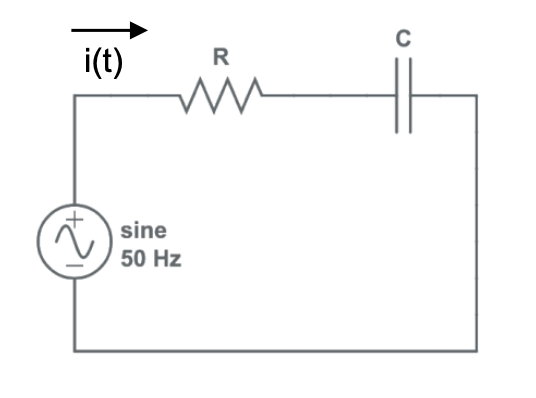
\includegraphics[width=4.16667in,height=\textheight,keepaspectratio]{media/ejercicio_PAU1.png}
\end{center}

\begin{enumerate}
\def\labelenumi{\alph{enumi})}
\tightlist
\item
  Obtener la corriente que atraviesa los elementos del circuito.
\item
  Determinar los valores de la capacidad \(C\) y de la reactancia
  capacitiva \(X_{C}\).
\item
  Calcular la potencia activa, reactiva y aparente y dibujar el
  triángulo de potencia. Determinar el valor del factor de potencia.
\end{enumerate}

\begin{tcolorbox}[enhanced jigsaw, breakable, colback=white, left=2mm, leftrule=.75mm, rightrule=.15mm, toprule=.15mm, colframe=quarto-callout-note-color-frame, arc=.35mm, bottomrule=.15mm, opacityback=0]

\textbf{Solución:} a) \(I = 8\) A.\\
b) \(X_C = 22,63\) \(\Omega\); \(C = 140,66\) \(\mu\)F.\\
c) \(P = 1000\) W; \(Q = -1448,32\) VAR (Capacitiva); \(S = 1760,01\)
VA; \(\cos\varphi = 0,57\).

\end{tcolorbox}

\subsection*{Problema 2}\label{problema-2}
\addcontentsline{toc}{subsection}{Problema 2}

Un circuito de corriente alterna conectado a un generador con una
tensión entre sus bornes de valor eficaz de \(220\) V y \(50\) Hz, tiene
en serie una resistencia de \(50\) \(\Omega\), una bobina de \(50\) mH y
un condensador de \(100\) \(\mu\)F.

\begin{enumerate}
\def\labelenumi{\alph{enumi})}
\tightlist
\item
  Dibujar el circuito y determinar la expresión \(v(t)\) del generador.
\item
  Determinar el valor de la impedancia del circuito. Razonar si se trata
  de una impedancia inductiva o capacitiva. Dibujar el triángulo de
  impedancias.
\item
  Calcular la caída de tensión e intensidad en cada uno de los
  componentes pasivos.
\item
  Calcular la potencia activa, reactiva y aparente. \emph{(Nota: Tómese
  para todo el problema como origen de fases la tensión del generador)}.
\end{enumerate}

\begin{tcolorbox}[enhanced jigsaw, breakable, colback=white, left=2mm, leftrule=.75mm, rightrule=.15mm, toprule=.15mm, colframe=quarto-callout-note-color-frame, arc=.35mm, bottomrule=.15mm, opacityback=0]

\textbf{Solución:} a) \(v(t) = 311,13 \cdot \text{sen}(100\pi t)\) V
(suponiendo fase 0).\\
b) \(\vec{Z} = 50 - j16,12 \Omega =52,53 \phase{-17,87º} \Omega\). Es
\textbf{capacitiva} (\(X_C > X_L\)).\\
c) \(\vec{U_R} = 209,5 \phase{17,87^{\circ}}\) V;
\(\vec{U_L} = 65,82 \phase{107,87^{\circ}}\) V;
\(\vec{U_C} = 133,37 \phase{-72,13^{\circ}}\) V.\\
d) \(P = 877,81\) W; \(Q = -283\) var (Capacitiva); \(S = 922,30\) VA.

\end{tcolorbox}

\subsection*{Problema 3}\label{problema-3}
\addcontentsline{toc}{subsection}{Problema 3}

En el circuito mostrado en la figura, donde \(U_{G}=100\) V (\(50\) Hz),
\(R=200\) \(\Omega\), \(L=50\) mH y \(C=15\) \(\mu\)F.

\begin{center}
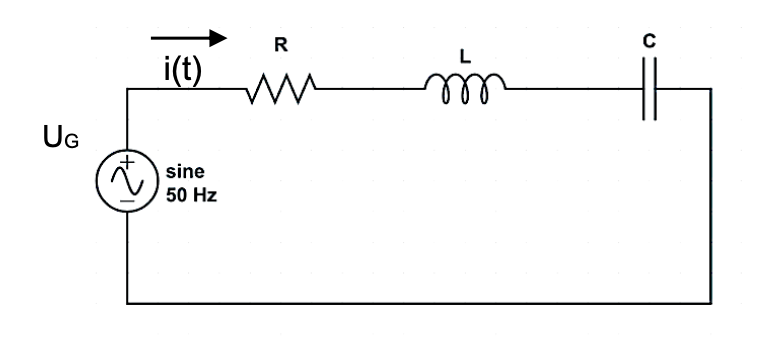
\includegraphics[width=4.16667in,height=\textheight,keepaspectratio]{media/ejercicio_PAU3.png}
\end{center}

\begin{enumerate}
\def\labelenumi{\alph{enumi})}
\tightlist
\item
  Determinar la intensidad proporcionada por la fuente en el circuito
  mostrado en la figura.
\item
  Dibujar el diagrama fasorial de tensión.
\end{enumerate}

\begin{tcolorbox}[enhanced jigsaw, breakable, colback=white, left=2mm, leftrule=.75mm, rightrule=.15mm, toprule=.15mm, colframe=quarto-callout-note-color-frame, arc=.35mm, bottomrule=.15mm, opacityback=0]

\textbf{Solución:} a) \(\vec{I} = 0,36\phase{44,49^{\circ}}\) A.

\end{tcolorbox}

\subsection*{Problema 4}\label{problema-4}
\addcontentsline{toc}{subsection}{Problema 4}

Se conecta una impedancia, \(Z=(40+j~31,41)\) \(\Omega\) a un generador
de corriente alterna de \(220\) V de tensión eficaz y \(50\) Hz de
frecuencia. Calcular:

\begin{enumerate}
\def\labelenumi{\alph{enumi})}
\tightlist
\item
  La potencia activa, la potencia reactiva y la potencia aparente y
  dibuje el triángulo de potencias.
\item
  La capacidad del condensador (\(\mu\)F) a conectar en paralelo con la
  impedancia para conseguir un factor de potencia de \(0,98\).
\end{enumerate}

\begin{tcolorbox}[enhanced jigsaw, breakable, colback=white, left=2mm, leftrule=.75mm, rightrule=.15mm, toprule=.15mm, colframe=quarto-callout-note-color-frame, arc=.35mm, bottomrule=.15mm, opacityback=0]

\textbf{Solución:} a) \(P = 749,22\) W; \(Q = 588,31\) var
\emph{(inductivo)}; \(S = 952,6\) VA.\\
b) \(C = 28,68\) \(\mu\)F.

\end{tcolorbox}

\subsection*{Problema 5}\label{problema-5}
\addcontentsline{toc}{subsection}{Problema 5}

Por una asociación serie de resistencia (R) e inductancia (L) en un
circuito eléctrico circula una intensidad de
\(i(t)=12 \cos(1200t+60^{\circ})\) mA, siendo el voltaje en los extremos
del conjunto de \(v(t)=0,8 \cos(1200t+85^{\circ})\) V. ¿Cuál es el valor
de la resistencia R y de la inductancia L?

\begin{tcolorbox}[enhanced jigsaw, breakable, colback=white, left=2mm, leftrule=.75mm, rightrule=.15mm, toprule=.15mm, colframe=quarto-callout-note-color-frame, arc=.35mm, bottomrule=.15mm, opacityback=0]

\textbf{Solución:} \(R = 60,42 \Omega\).\\
\(L = 23,47\) mH.

\end{tcolorbox}

\subsection*{Problema 6}\label{problema-6}
\addcontentsline{toc}{subsection}{Problema 6}

Un circuito doméstico de \(230\) V eficaces a \(50\) Hz alimenta dos
lámparas de \(75\) W con un factor de potencia unidad y un motor que
consume \(500\) VA con un factor de potencia \(0,78\) inductivo.

\begin{enumerate}
\def\labelenumi{\alph{enumi})}
\tightlist
\item
  Dibujar el circuito, representando cada carga mediante una impedancia
  e incluyendo el interruptor de cada carga.
\item
  Determinar la corriente total cuando todas las cargas operan de forma
  simultánea.
\item
  ¿Qué condensador conectado en paralelo con las cargas dará un factor
  de potencia unidad?
\end{enumerate}

\begin{tcolorbox}[enhanced jigsaw, breakable, colback=white, left=2mm, leftrule=.75mm, rightrule=.15mm, toprule=.15mm, colframe=quarto-callout-note-color-frame, arc=.35mm, bottomrule=.15mm, opacityback=0]

\textbf{Solución:} b) \(\vec{I_{total}} = 2,71\phase{-30,09^{\circ}}\)
A.\\
c) \(C = 18,6\) \(\mu\)F.

\end{tcolorbox}

\subsection*{Problema 7}\label{problema-7}
\addcontentsline{toc}{subsection}{Problema 7}

En una red de alimentación de \(230\) V y \(50\) Hz se encuentra
conectado un motor asíncrono monofásico que consume una potencia de
\(7,4\) kW con un factor de potencia de \(0,8\) inductivo. Determinar:

\begin{enumerate}
\def\labelenumi{\alph{enumi})}
\tightlist
\item
  Capacidad de la batería de condensadores que hay que conectar en
  paralelo con el conjunto de receptores para corregir el factor de
  potencia a \(0,95\).
\item
  Intensidad consumida antes de conectar la batería de condensadores.
\item
  Intensidad consumida después de conectar la batería de condensadores.
\end{enumerate}

\begin{tcolorbox}[enhanced jigsaw, breakable, colback=white, left=2mm, leftrule=.75mm, rightrule=.15mm, toprule=.15mm, colframe=quarto-callout-note-color-frame, arc=.35mm, bottomrule=.15mm, opacityback=0]

\textbf{Solución:} a) \(C = 187,64\) \(\mu\)F.\\
b) \(I_{antes} = 40,21\) A.\\
c) \(I_{después} = 33,86\) A.

\end{tcolorbox}

\subsection*{Problema 8}\label{problema-8}
\addcontentsline{toc}{subsection}{Problema 8}

Determinar el triángulo de potencias de un receptor eléctrico al que se
le aplica una tensión de \(u(t)=290 \text{sen}(\omega t-90^{\circ})\) V
y absorbe una intensidad de \(i(t)=17 \text{sen}(\omega t-30^{\circ})\)
A.

\begin{tcolorbox}[enhanced jigsaw, breakable, colback=white, left=2mm, leftrule=.75mm, rightrule=.15mm, toprule=.15mm, colframe=quarto-callout-note-color-frame, arc=.35mm, bottomrule=.15mm, opacityback=0]

\textbf{Solución:} \(S = 2464,82\) VA.\\
\(P = 1232,5\) W.\\
\(Q = -2134,6\) var (Capacitiva).

\end{tcolorbox}

\subsection*{Problema 9}\label{problema-9}
\addcontentsline{toc}{subsection}{Problema 9}

El circuito de la figura KM representa un interruptor magnetotérmico
bipolar que protege la instalación. Determinar la corriente mínima que
debe soportar el interruptor para que en condiciones normales de
funcionamiento no se dispare. ¿Cuál es el factor de potencia del
conjunto de la instalación?

\begin{center}
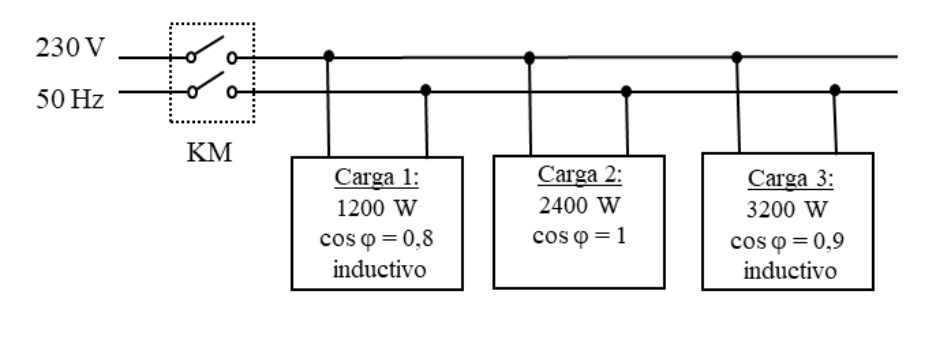
\includegraphics[width=4.16667in,height=\textheight,keepaspectratio]{media/ejercicio_PAU9.png}
\end{center}

\begin{itemize}
\tightlist
\item
  Carga 1: \(1200\) W, \(\cos\varphi=0.8\) inductivo.
\item
  Carga 2: \(2400\) W, \(\cos\varphi=1\).
\item
  Carga 3: \(3200\) W, \(\cos\varphi=0,9\) inductivo.
\end{itemize}

\begin{tcolorbox}[enhanced jigsaw, breakable, colback=white, left=2mm, leftrule=.75mm, rightrule=.15mm, toprule=.15mm, colframe=quarto-callout-note-color-frame, arc=.35mm, bottomrule=.15mm, opacityback=0]

\textbf{Solución:} \(\vec{I}=31,39\phase{-19,80^{\circ}}\) A.\\
Factor de potencia: \(\cos\varphi = 0,94\).

\end{tcolorbox}

\subsection*{Problema 10}\label{problema-10}
\addcontentsline{toc}{subsection}{Problema 10}

Un generador de frecuencia variable de corriente alterna a \(230\) V y
\(50\) Hz, alimenta un circuito RLC paralelo formado por una \(R=40\)
\(\Omega\), una inductancia de \(L=100\) mH y un condensador de
\(C=300\) \(\mu\)F, calcular:

\begin{enumerate}
\def\labelenumi{\alph{enumi})}
\tightlist
\item
  La intensidad de corriente que circula por cada una de las ramas del
  circuito.
\item
  El factor de potencia del circuito.
\item
  Las potencias activa, reactiva y aparente del circuito.
\item
  El valor de la frecuencia necesaria para que el factor de potencia de
  este circuito sea la unidad.
\end{enumerate}

\begin{tcolorbox}[enhanced jigsaw, breakable, colback=white, left=2mm, leftrule=.75mm, rightrule=.15mm, toprule=.15mm, colframe=quarto-callout-note-color-frame, arc=.35mm, bottomrule=.15mm, opacityback=0]

\textbf{Solución:} a) \(\vec{I_R} = 5,75\phase{0^{\circ}}\) A;
\(\vec{I_L} = 7,32\phase{-90^{\circ}}\) A;
\(\vec{I_C} = 21,68\phase{90^{\circ}}\) A.\\
b) \(\cos\varphi = 0,37\) (Capacitivo).\\
c) \(P = 1322,5\) W; \(Q = -3303,18\) var; \(S = 3558,1\) VA.\\
d) Resonancia (\(X_L = X_C\)): \(f = \frac{1}{2\pi\sqrt{LC}} = 29,06\)
Hz.

\end{tcolorbox}




\end{document}
